\chapter{Supervised multivariate discretization and factor levels merging} \label{chap4}


To improve prediction accuracy and interpretability of logistic regression-based scorecards, a preprocessing step quantizing both continuous and categorical data is usually performed: continuous features are discretized by assigning factor levels to intervals and, if numerous, levels of categorical features are grouped. However, a better predictive accuracy can be reached by embedding this quantization estimation step directly into the predictive estimation step itself. By doing so, the predictive loss has to be optimized on a huge and untractable discontinuous quantization set. To overcome this difficulty, I introduced a specific two-step optimization strategy: first, the optimization problem is relaxed by approximating discontinuous quantization functions by smooth functions; second, the resulting relaxed optimization problem is solved either \textit{via} a particular neural network and stochastic gradient descent or a \gls{sem} algorithm. The strategy gives then access to good candidates for the original optimization problem after a straightforward \textit{maximum a posteriori} procedure to obtain cutpoints. The good performances of this approach, which we call \textit{glmdisc}, are illustrated on simulated and real data from the UCI library and \gls{cacf}. The results show that practitioners finally have an automatic all-in-one tool that answers their recurring needs of quantization for predictive tasks.
 
 \section{Motivation}

As stated by~\cite{hosmer2013applied} and illustrated in this manuscript, in many application contexts (credit scoring, biostatistics, {\it etc.}), logistic regression is widely used for its simplicity, decent performance and interpretability in predicting a binary outcome given predictors of different types (categorical, continuous). However, to achieve  higher interpretability, continuous predictors are sometimes discretized so as to produce a ``scorecard'', \textit{i.e.}\ a table assigning a grade to an applicant in credit scoring (or a patient in biostatistics, {\it etc.}) depending on its predictors being in a given interval.

Discretization is also an opportunity for reducing the (possibly large) modeling bias which can appear in logistic regression as a result of the linearity assumption on the continuous predictors in the model. Indeed, this restriction can be overcome by approximating the true predictive mapping with a step function where the tuning of the steps and their sizes allows more flexibility. However, the resulting increase of the number of parameters can lead to an increase in variance (overfitting) as shown in \cite{yang2009discretization}. Thus, a precise tuning of the discretization procedure is required. Likewise when dealing with categorical features which take numerous levels, their respective regression coefficients suffer from high variance. A straightforward solution formalized by \cite{maj2015delete} is to merge their factor levels which leads to less coefficients and therefore less variance. 

From now on, the generic term quantization will stand for both discretization of continuous features and level grouping of categorical ones. Its aim is to improve the prediction accuracy. Such a quantization can be seen as a special case of \textit{representation learning}, but suffers from a highly combinatorial optimization problem whatever the predictive criterion used to select the best quantization. The present work proposes a strategy to overcome these combinatorial issues by invoking a relaxed alternative of the initial quantization problem leading to a simpler estimation problem since it can be easily optimized by either a specific neural network or an \gls{sem} algorithm. These relaxed versions serve as a plausible quantization provider related to the initial criterion after a classical thresholding (\textit{maximum a posteriori}) procedure.

The outline of this chapter is the following. In the next section, we illustrate cases where quantization is either beneficial or detrimental depending on the data generating mechanism. In the subsequent section, we formalize both continuous and categorical quantization. Selecting the best quantization in a predictive setting is reformulated as a model selection problem on a huge discrete space which size is precisely derived. In Section~\ref{sec:proposal}, a particular neural network architecture is used to optimize a relaxed version of this criterion and propose good quantization candidates. At first, an \gls{sem} procedure was proposed to solve the quantization problem and is reported in section~\ref{sec:sem}. Section~\ref{sec:experiments} is dedicated to numerical experiments on both simulated and real data from the field of Credit Scoring, highlightening the good results offered by the use of the two new methods without any human intervention. A final section concludes the work by stating also new challenges.


\section{Illustration of the bias-variance quantization tradeoff}
 
 
 
 
 
 
 
\section{Quantization as a combinatorial challenge} \label{sec:model_selection}

\subsection{Quantization: definition}

\paragraph{General principle}

The quantization procedure consists in turning a $d$-dimensional raw vector of continuous and/or categorical features $\glssymbol{bx} = (\glssymbol{x}_1, \ldots, \glssymbol{x}_d)$ into a $d$-dimensional categorical vector via a component wise mapping $\q=(\q_j)_1^d$:
\[\q(\glssymbol{bx})=(\q_1(\glssymbol{x}_1),\ldots,\q_d(\glssymbol{x}_d)),\]
where each of the $\q_j$'s is a vector of $m_j$ dummies: 
\begin{equation}\label{eq:qj}
q_{j,h}(\cdot) =  1 \text{ if } x_j \in C_{j,h}, 0 \text{ otherwise, } 1 \leq h \leq m_j,
\end{equation}
where $m_j$ is an integer and the sets $C_{j,h}$ are defined with respect to each feature type as we describe just below.
\paragraph{Raw continuous features} If $\glssymbol{x}_j$ is a continuous component of $\glssymbol{bx}$, quantization $\q_j$ has to perform a discretization of $\glssymbol{x}_j$ and the $C_{j,h}$'s, $1\le h\le m_j$, are contiguous intervals  
\begin{equation}\label{eq:Cjhcont}
C_{j,h}=(c_{j,h-1},c_{j,h}]
\end{equation}
where $c_{j,1},\ldots,c_{j,m_j-1}$ are increasing numbers called cutpoints, $c_{j,0}=-\infty$, $c_{j,m_j}=\infty$.

For example, the quantization of the unit segment in thirds would be defined as $m_j=3$, $c_{j,1} = 1/3$, $c_{j,2} = 2/3$ and subsequently $\q_j(0.1) = (1,0,0)$.
\paragraph{Raw categorical features} If $x_j$ is a categorical component of $\glssymbol{bx}$, quantization $\q_j$ consists in grouping levels of $\glssymbol{x}_j$ and the $C_{j,h}$s form a partition of the set, say $\{1,\ldots,l_j\}$, of levels of $\glssymbol{x}_j$: 
\begin{equation*}
\bigsqcup_{h=1}^{m_j}C_{j,h}=\{1,\ldots,l_j\}.
\end{equation*}
For example, the grouping of levels encoded as ``1'' and ``2'' would yield $C_{j,1} = \{1,2\}$ such that $\q_j(1) = \q_j(2) = (1,0,\ldots,0)$.

\paragraph{Notations for the quantization family}

In both continuous and categorical cases, keep in mind that $m_j$ is the dimension of $\q_j$. For notational convenience, the (global) order of the quantization $\q$ is set as 
\[|\q|=\sum_{j=1}^d m_j.\]
The space where quantizations $\q$ live will be denoted by $\Q$ in the sequel.



\subparagraph{Cardinality of the quantization family in the continuous case}

 \# TODO
 
 
 \subparagraph{Cardinality of the quantization family in the categorical case}

 
  \# TODO



\paragraph{Literature review}

The current practice of quantization is prior to any predictive task, thus ignoring its consequences on the final predictive ability. It consists in optimizing a heuristic criterion, often totally unrelated (unsupervised methods) or at least explicitly (supervised methods) to prediction, and mostly univariate (each feature is quantized irrespective of other features' values). The cardinality of the quantization space $\Q$ can be calculated explicitely w.r.t.\ $d$, $(m_j)_1^d$ and, for categorical features, $l_j$. It is huge, so that a greedy approach is intractable and such heuristics are needed.
Many algorithms have thus been designed and a review of approximatively 200 discretization strategies, gathering both criteria and related algorithms, can be found in \cite{ramirez2016data}. For factor levels grouping, we found no such taxonomy, but some discretization methods, \textit{e.g.}\ $\chi^2$ independence test-based methods can be naturally extended to this type of quantization, which is for example what the CHAID algorithm, proposed by~\cite{kass1980exploratory} and applied to each categorical feature, relies on.


\# TODO


\subsection{Quantization embedded in a predictive process}

\paragraph{Logistic regression on quantized data}

Quantization is a widespread preprocessing step to perform a learning task consisting in predicting, say, a binary variable $\glssymbol{y}\in\{0,1\}$, from a quantized predictor  $\q(\glssymbol{bx})$, through, say, a parametric conditional distribution $p_{\glssymbol{bth}}(\glssymbol{y}|\q(\glssymbol{bx}))$ like logistic regression. Considering quantized data instead of raw data has a double benefit. First, the quantization order $|\q|$ acts as a tuning parameter for controlling the model's flexibility and thus the bias/variance trade-off of the estimate of the parameter $\glssymbol{bth}$ (or of its predictive accuracy) for a given dataset. This claim becomes clearer with the example of logistic regression we focus on, as a still very popular model for many practitioners. It is classically described by
\begin{equation}
    \label{eq:reglogq}
\ln \left( \dfrac{p_{\glssymbol{bth}}(1|\q(\glssymbol{bx}))}{1 - p_{\glssymbol{bth}}(1|\q(\glssymbol{bx}))} \right) = \theta_0 + \sum_{j=1}^d \glssymbol{bth}_j' \cdot \q_j(\glssymbol{x}_j),
\end{equation}
where $\glssymbol{bth} = (\theta_{0},(\glssymbol{bth}_j)_1^d) \in \mathbb{R}^{|\q|+1}$ and $\glssymbol{bth}_j = (\theta_{j}^{1},\dots,\theta_{j}^{m_j})$ with $\theta_{j}^{m_j} = 0$, $j=1 \ldots d$, for identifiability reasons.
Second, at the practitioner level, the previous tuning of $|\q|$ through each feature's quantization order $m_j$, especially when it is quite low, allows an easier interpretation of the most important predictor values involved in the predictive process. Denoting the dataset by $(\glssymbol{bbx},\glssymbol{bby})$, with $\glssymbol{bbx}=(\glssymbol{bx}_1,\ldots,\glssymbol{bx}_n)$ and $\glssymbol{bby}=(\glssymbol{y}_1,\ldots,\glssymbol{y}_n)$, the log-likelihood 
\begin{equation}
\label{eq:lq}
\ell_{\q}(\glssymbol{bth} ; (\glssymbol{bbx},\glssymbol{bby}))=\sum_{i=1}^n \ln p_{\glssymbol{bth}}(\glssymbol{y}_i|\q(\glssymbol{bx}_i))
\end{equation}
provides a Maximum Likelihood estimator $\hat{\glssymbol{bth}}_\q$ of $\glssymbol{bth}$ for a given quantization $\q$. For the rest of the chapter and consistently with the manuscript, the approach is exemplified with logistic regression as $p_{\glssymbol{bth}}$ but it can be applied to any other predictive model, as will be recalled in the concluding section.



\paragraph{Quantization as a model selection problem}

As dicussed in the previous section, and emphasized in the literature review, quantization is often a preprocessing step; however, quantization can be embedded directly in the predictive model. Continuouing our logistic example, a standard information criteria such as the BIC (\cite{BIC}) can be used to select the best quantization $\q$:
\begin{equation}
    \label{eq:BICq}
    \hat{\q}=\argmax_{\q \in \Q} \left\{\ell_\q(\hat{\glssymbol{bth}}_\q ; (\glssymbol{bbx},\glssymbol{bby}))-\frac12 \nu_\q \ln (n)\right\}
\end{equation}
where $\nu_\q$ is the number of continuous parameters to be estimated in the $\glssymbol{bth}$-parameter space. Note however that an exhaustive search of $\hat{\q}\in\Q$ is an intractable task due to its highly combinatorial nature. For example, with $d=10$ categorical features with $l_j = 4$ levels each, $|\Q|$ is given by the Stirling number of the second kind to the power $d$, which is approx.\ $6 \cdot 10^{11}$. Anyway, the optimization~(\ref{eq:BICq}) requires a new specific strategy that we describe in the next section.

\# TODO : référence problèmes BIC et nombre de modèles dépendant de n

\paragraph{Remark on model identifiability}

The shifting of cutpoints (\ref{eq:Cjhcont}) anywhere strictly between two successive raw values of a given continuous feature induce the same quantization, as was discussed thoroughly in Paragraph~\ref{par:cardinality}. Thus, the identifiability of such quantizations is obtained from the dataset $\glssymbol{bbx}$ by fixing arbitrary cutpoints between successive data values, feature by feature. The continuous part of $\Q$ then becomes a discrete set.



 \section{The proposed neural network based quantization}
\label{sec:proposal}

\subsection{A relaxation of the optimization problem}

In this section, we propose to relax the constraints on $\q_j$ to simplify the search of $\hat{\q}$. Indeed, the derivatives of $\q_j$ are zero almost everywhere and consequently a gradient descent cannot be directly applied to find an optimal quantization.

\paragraph{Smooth approximation of the quantization mapping}

A classical approach is to replace the binary functions $q_{j,h}$ (see Equation (\ref{eq:qj}))  by smooth parametric ones  with a simplex condition, namely with $\ag_j=(\ag_{j,1},\ldots, \ag_{j,m_j})$:
%\begin{equation}
\begin{equation*}
    %\label{eq:qaj}
    {\q_{\ag_j}(\cdot)=\left(q_{\ag_{j,h}}(\cdot)\right)_{h=1}^{m_j} \text{ with } \sum_{h=1}^{m_j}q_{\ag_{j,h}}(\cdot)=1 \text{ and } 0 \leq q_{\ag_{j,h}}(\cdot) \leq 1,}
\end{equation*}
%\end{equation}
where functions $q_{\ag_{j,h}}(\cdot)$, properly defined hereafter for both continuous and categorical features, represent a fuzzy quantization in that, here, each level $h$ is weighted by $q_{\ag_{j,h}}(\cdot)$ instead of being selected once and for all as in (\ref{eq:qj}). The resulting fuzzy quantization for all components depends on the global parameter $\ag = (\ag_1, \ldots, \ag_d)$ and is denoted by $\q_{\ag}(\cdot)=\left(\q_{\ag_j}(\cdot)\right)_{j=1}^d$. This approximation is justified by the following arguments. From a deterministic point of view, denoting by $\tilde{\Q}$ the space of $\q_{\ag}$, we have $\Q \subset \widetilde{\Q}$. From a statistical point of view, under standard regularity conditions and with a suitable estimation procedure (see later for the proposed estimation procedure), we have consistency of $(\q_{\hat{\ag}}, \hat{\glssymbol{bth}})$ towards $(\q,\glssymbol{bth})$. From an empirical point of view, we will see in Section~\ref{sec:experiments} and in particular in Figure~\ref{fig:MAP}, that this smooth approximation $\q_{\ag}$ converges towards ``hard'' quantizations\footnote{Up to a permutation on the labels $h=1 \ldots m_j$ to recover the ordering in $C_{j,h}$ (see Eq. (\ref{eq:Cjhcont})).} $\q$.



 {\bf For continuous features}, we set for $\ag_{j,h} = (\alpha^0_{j,h},\alpha^1_{j,h}) \in \mathbb{R}^2$
\[q_{\ag_{j,h}}(\cdot) = \frac{\exp(\alpha^0_{j,h} + \alpha^1_{j,h}  \cdot)}{\sum_{g=1}^{m_j} \exp(\alpha^0_{j,g} + \alpha^1_{j,g}  \cdot)}\]
where $\ag_{j,m_j}$ is set to $(0,0)$ for identifiability reasons.




{\bf For categorical features}, we set for $\ag_{j,h}=\left(\alpha_{j,h}(1),\ldots, \alpha_{j,h}(l_j)\right) \in \mathbb{R}^{l_j}$
\[q_{\ag_{j,h}}(\cdot) = \frac{\exp\left(\alpha_{j,h}(\cdot)\right)}{\sum_{g=1}^{m_j} \exp\left(\alpha_{j,g}(\cdot)\right)}\]
where $l_j$ is the number of levels of the categorical feature $\glssymbol{x}_j$.

\paragraph{Parameter estimation}

With this new fuzzy quantization, the logistic regression for the predictive task is then expressed as
\begin{equation}
    \label{eq:reglogqa}
    \ln \left( \dfrac{p_{\glssymbol{bth}}(1|\q_{\ag} (\glssymbol{bx}))}{1 - p_{\glssymbol{bth}}(1|\q_{\ag} (\glssymbol{bx}))} \right) = \theta_0 + \sum_{j=1}^d {\glssymbol{bth}_j' \cdot \q_{\ag_{j}}(x_j)},
\end{equation}
where $\q$ has been replaced by $\q_{\ag}$ from Equation~(\ref{eq:reglogq}).
Note that as $\q_{\ag}$ is a sound approximation of $\q$ (see above), this logistic regression in $\q_{\ag}$ is consequently a good approximation of the logistic regression in $\q$ from Equation~(\ref{eq:reglogq}). The relevant log-likelihood is here 
\begin{equation}
    \label{eq:lqa}
    \ell_{\q_{\ag}}(\glssymbol{bth} ; (\glssymbol{bbx},\glssymbol{bby}))=\sum_{i=1}^n \ln p_{\glssymbol{bth}}(y_i|\q_{\bm{\alpha}}(\bm{x}_i))
\end{equation}
and can be used as a tractable substitute for (\ref{eq:lq}) to solve the original optimization problem (\ref{eq:BICq}), where now both $\ag$ and $\glssymbol{bth}$ have to be estimated, which is discussed in the next section. We wish to maximize the log-likelihood (\ref{eq:reglogqa}) which would yield parameters $(\hat{\ag},\hat{\glssymbol{bth}})$; these are consistent if the model is well-specified (\textit{i.e.}\ there is a ``true'' quantization under classical regularity conditions). To ``push'' $\widetilde{\Q}$ further into $\Q$, we deduce $\hat{\q}$ from a \textit{maximum a posteriori} procedure applied to $\q_{\hat{\ag}}$:
\begin{equation}
    \label{eq:ht}
    \hat{q}_{j,h}(x_j) = 1 \text{ if } h = \argmax_{1 \leq h' \leq m_j} q_{\hat{\ag}_{j,h'}}, 0 \text{ otherwise.}
\end{equation}
If there are several levels $h$ that satisfy (\ref{eq:ht}), we simply take the level that corresponds to smaller values of $x_j$ to be in accordance with the definition of $C_{j,h}$ in Equation~(\ref{eq:Cjhcont}). This {\it maximum a posteriori} principle will be exemplified in Figure~\ref{fig:MAP} on simulated data.


\subsection{A neural network-based estimation strategy} \label{sec:estim}

\paragraph{Neural network architecture}

To estimate parameters $\ag$ and $\glssymbol{bth}$ in the model (\ref{eq:reglogqa}), a particular neural network architecture can be used. The most obvious part is the output layer that must produce $p_{\glssymbol{bth}}(1|\q_{\ag}(\glssymbol{bx}))$ which is equivalent to a densely connected layer with a sigmoid activation $\sigma (\cdot)$.

For a continuous feature $\glssymbol{x}_j$ of $\glssymbol{bx}$, the combined use of $m_j$ neurons including affine transformations and softmax activation obviously yields $\q_{\ag_{j}}(x_j)$. Similarly, an input categorical feature $\glssymbol{x}_j$ with $l_j$ levels is equivalent to $l_j$ binary input neurons (presence or absence of the factor level). These $l_j$ neurons are densely connected to $m_j$ neurons without any bias term and a softmax activation. The softmax outputs are next aggregated via the summation in model (\ref{eq:reglogqa}), say $\Sigma_{\glssymbol{bth}}$ for short, and then the sigmoid function $\sigma$ gives the final output. All in all, the proposed model is straightforward to optimize with a simple neural network, as shown in Figure~\ref{fig:nn}.


\def\layersep{2.5cm}

\begin{figure}[h!]
\centering
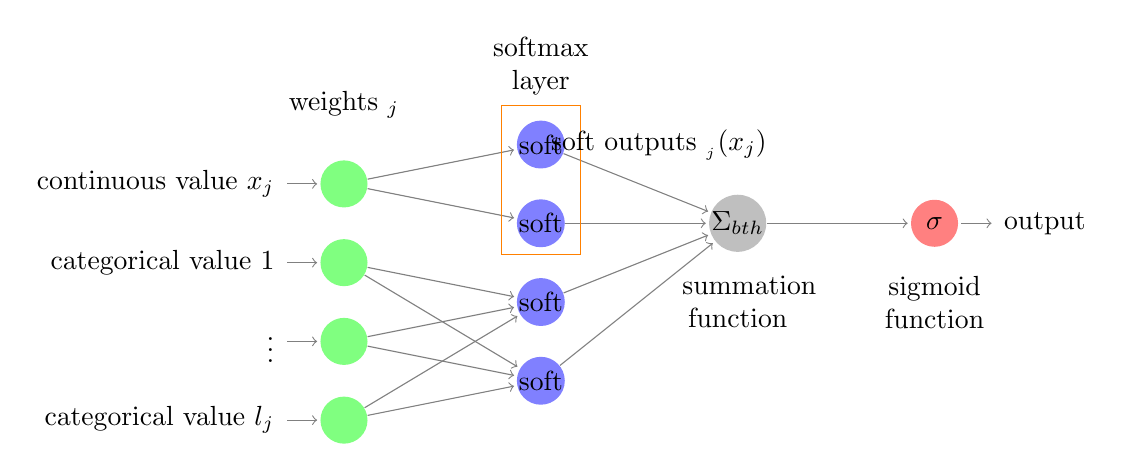
\begin{tikzpicture}[shorten >=1pt,->,draw=black!50, node distance=\layersep]
    \tikzstyle{every pin edge}=[<-,shorten <=1pt]
    \tikzstyle{neuron}=[circle,fill=black!25,minimum size=17pt,inner sep=0pt]
    \tikzstyle{input neuron}=[neuron, fill=green!50];
    \tikzstyle{output neuron}=[neuron, fill=red!50];
    \tikzstyle{hidden neuron}=[neuron, fill=blue!50];
    \tikzstyle{annot} = [text width=4em, text centered]
    \tikzstyle{annotrectangle} = [text width=8em, text centered]


        \node[input neuron, pin=left:continuous value $x_j$] (I-1) at (0,-1) {};
        
        \node[input neuron, pin=left:categorical value $1$] (I-2) at (0,-2) {};
        \node[input neuron, pin=left:$\vdots$] (I-3) at (0,-3) {};
        \node[input neuron, pin=left:categorical value $l_j$] (I-4) at (0,-4) {};

    % Draw the hidden layer nodes
    \foreach \name / \y in {1,...,2}
        \path[yshift=0.5cm]
            node[hidden neuron] (H-\name) at (\layersep,-\y cm) {soft};

    \foreach \name / \y in {3,...,4}
        \path[yshift=0.5cm]
            node[hidden neuron] (H-\name) at (\layersep,-\y cm) {soft};
            
    % Draw the sum layer node 
    
    \node[neuron, right of=H-2] (S) {$\Sigma_{\glssymbol{bth}}$};

    % Draw the output layer node
    
    \node[output neuron,pin={[pin edge={->}]right:output}, right of=S] (O) {$\sigma$};
    
    %\node[output neuron,pin={[pin edge={->}]right:Output}, right of=H-2] (O) {$\sigma(\cdot)$};
    
    

    % Connect every node in the input layer with every node in the
    % hidden layer.
%    \foreach \source in {1,...,4}
        \foreach \dest in {1,2}
            \path (I-1) edge (H-\dest);

        \foreach \dest in {3,4}
            \path (I-2) edge (H-\dest);
        \foreach \dest in {3,4}
            \path (I-3) edge (H-\dest);
        \foreach \dest in {3,4}
            \path (I-4) edge (H-\dest);

        % \foreach \dest in {5,6}
        %     \path (I-3) edge (H-\dest);

    % Connect every node in the hidden layer with the output layer
    \foreach \source in {1,...,4}
        \path (H-\source) edge (S);
        
    % connect Sigma with sigma
    \path (S) edge (O);

    % Annotate the layers
    \node[annot,above of=H-1, node distance=1cm] (hl) {softmax layer};
    \node[annot,above of=I-1,node distance=1cm] {weights $\ag_j$};
    %\node[annot,right of=hl] (s) {};
    \node[annot, below of=O, node distance=1cm] (s) {sigmoid function};
    \node[annot, below of=S,node distance=1cm] {summation function};
    
    \draw [orange] (2,0) rectangle (3,-1.9);
    % \draw [red] (2,-2) rectangle (3,-4);
    
    \node[annotrectangle,right of=H-1, node distance=1.5cm] {soft outputs $\q_{\ag_j}(x_j)$}; 

\end{tikzpicture}
\caption{Proposed shallow architecture to maximize (\ref{eq:lqa}).}
\label{fig:nn}
\end{figure}


\paragraph{Stochastic gradient descent as a quantization provider}

By relying on a stochastic gradient descent, the smoothed likelihood (\ref{eq:lqa}) can be maximized over $\left(\ag, \glssymbol{bth} \right)$. The results should be close to the maximizers of the original likelihood (\ref{eq:lq}) if the model is well-specified, when there is a true underlying quantization. In the mis-specified model case, there is no such guarantee. Therefore, to be more conservative, we evaluate at each training epoch $(t)$ the quantization $\hat{\q}^{(t)}$ resulting from the \textit{maximum a posteriori} procedure explicited in Equation~(\ref{eq:ht}), then classicaly estimate the logistic regression parameter \textit{via} maximum likelihood, as done in Equation~(\ref{eq:lq}):
\[\glssymbol{bth}^{(t)} = \argmin_{\glssymbol{bth}} \ell_{\q^{(t)}}(\glssymbol{bth}; (\glssymbol{bbx},\glssymbol{bby}))\]
and the resulting $\mbox{BIC}^{(t)}$ as in (\ref{eq:BICq}). If $T$ is a given maximum number of iterations of the stochastic gradient descent algorithm, the quantization retained at the end is then determined by the optimal epoch
\[t_*=\argmin_{t\in \{1,\ldots, T\}} \mbox{BIC}^{(t)}.\]
 
\paragraph{Choosing an appropriate number of levels}

Concerning now the number of intervals or factor levels $\boldsymbol{m} = (m_j)_1^d$, they have also to be estimated since in practice they are unknown. Looping over all candidates $\boldsymbol{m}$ is intractable. But in practice, by relying on the \textit{maximum a posteriori} procedure developed in Equation~(\ref{eq:ht}), we might drop a lot of unseen factor levels, \textit{e.g.}\ if $q_{\ag_{j,h}}(x_{i,j}) \ll 1$ for all training observations $\glssymbol{xij}$, the level $h$ ``vanishes'', \textit{i.e.}\ $\hat{q}_{j,h} = 0$. In practice, we recommend to start with a user-chosen $\bm{m}=\boldsymbol{m}_{\max}$ and we will see in the experiments of Section~\ref{sec:experiments} that the proposed approach is able to explore small values of $\boldsymbol{m}$ and to select a value $\hat{\boldsymbol{m}}$ drastically smaller than $\boldsymbol{m}_{\max}$. This phenomenon, which reduces the computational burden of the quantization task, is also illustrated in the next section.




\section{An \gls{sem} approach} \label{sec:sem}
 
 
 
 
 
 
 \section{Numerical experiments} \label{sec:experiments}

This section is divided into three complementary parts to assess the validity of our proposal, that we call hereafter \textit{glmdisc}. First, simulated data are used to evaluate its ability to recover the true data generating mechanism. Second, the predictive quality of the new learned representation approach is illustrated on several classical benchmark datasets from the UCI library. Third, we use it on \textit{Credit Scoring} datasets provided by Credit Agricole Consumer Finance, a major European company in the consumer credit market. The Python notebooks of all experiments, excluding the confidential real data, can be found on the first author's website.

\subsection{Simulated data: empirical consistency and robustness}

We focus here on discretization of continuous features (similar experiments could be conducted on categorical ones). Two continuous features $x_1$ and $x_2$ are sampled from the uniform distribution on $[0,1]$ and discretized by using
\[\q_1(\cdot)=\q_2(\cdot) = (\mathds{1}_{]-\infty,1/3]}(\cdot),\mathds{1}_{]1/3,2/3]}(\cdot),\mathds{1}_{]2/3,\infty]}(\cdot)).\]
Here, following (\ref{eq:Cjhcont}), we have $d=2$ and $m_1=m_2=3$ and the cutpoints are $c_{j,1}=1/3$ and $c_{j,2}=2/3$ for $j=1,2$. Setting $\glssymbol{bth}=(0,-2,2,0,-2,2,0)$, the target feature $y$ is then sampled from $p_{\glssymbol{bth}}(\cdot | \q(\glssymbol{bbx}))$ via the logistic model (\ref{eq:reglogq}).

From the \textit{glmdisc} algorithm, we studied three cases:
\begin{enumerate}[(a)]
    \item First, the quality of the cutoff estimator $\hat{c}_{j,2}$ of $c_{j,2} = 2/3$ is assessed when the starting maximum number of intervals per discretized continuous feature is set to its true value $m_1=m_2= 3$;
    \item Second, we estimated the number of intervals $\hat{m}_1$ of $m_1=3$ when the starting maximum number of intervals per discretized continuous feature is set to $m_{\text{max}} = 10$; 
    \item Last, we added a third feature $x_3$ also drawn uniformly on $[0,1]$ but uncorrelated to $y$ and estimated the number $\hat{m}_3$ of discretization intervals selected for $x_3$. The reason is that a non-predictive feature which is discretized or grouped into a single value is \textit{de facto} excluded from the model, and this is a positive side effect.
\end{enumerate}
From a statistical point of view, experiment (a) assesses the empirical consistency of the estimation of $C_{j,h}$, whereas experiments (b) and (c) focus on the consistency of the estimation of $m_j$. The results are summarized in Table~\ref{tab:estim_precision} where 95\% confidence intervals (CI) are given, with a varying sample size. Note in particular that the slight underestimation in (b) is a classical consequence of the BIC criterion on small samples. 
\begin{table}[h!]
    \centering
\begin{tabular}{llll}
Sample size & (a) $\hat{c}_{j,2}$ & (b) $\hat{m}_1$ & (c) $\hat{m}_3$\\
\hline
$n = 1,000$ & $[0.656,0.666]$ & $[2.679,2.941]$ & $[1.326,1.554]$ \\
$n = 10,000$ & $[0.666,0.666]$ & $[3.000,3.000]$ & $[1.399,1.621]$
\end{tabular}
    \caption{(a) CI of $\hat{c}_{j,2}$ for $c_{j,2} = 2/3$. (b) CI of $\hat{m}$ for $m_1=3$. (c) CI of $\hat{m}_3$ for $m_3=1$.}
    \label{tab:estim_precision}
\end{table}

 \newlength\figureheight
 \newlength\figurewidth
 \setlength\figureheight{4cm}
 \setlength\figurewidth{14cm}
 
  \begin{figure}
    \centering
    \begin{subfigure}[t]{\textwidth}
        \centering
        % This file was created by matplotlib2tikz v0.6.18.
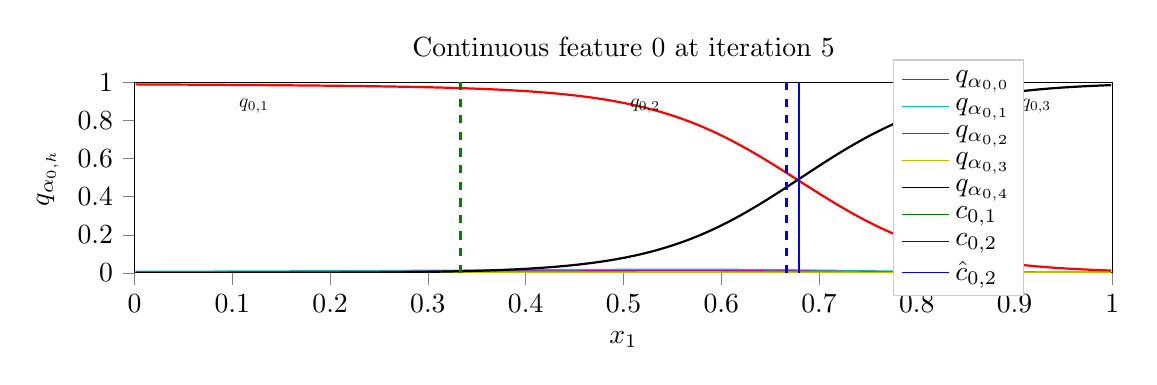
\begin{tikzpicture}

\definecolor{color0}{rgb}{0,0.75,0.75}
\definecolor{color1}{rgb}{0.75,0,0.75}
\definecolor{color2}{rgb}{0.75,0.75,0}

\begin{axis}[
height=\figureheight,
legend cell align={left},
legend entries={{${q}_{\bm{\alpha}_{0,0}}$},{${q}_{\bm{\alpha}_{0,1}}$},{${q}_{\bm{\alpha}_{0,2}}$},{${q}_{\bm{\alpha}_{0,3}}$},{${q}_{\bm{\alpha}_{0,4}}$},{$c_{0,1}$},{$c_{0,2}$},{$\hat{c}_{0,2}$}},
legend style={at={(0.91,0.5)}, anchor=east, draw=white!80.0!black},
tick align=outside,
tick pos=left,
title={Continuous feature 0 at iteration 5},
width=\figurewidth,
x grid style={white!69.01960784313725!black},
xlabel={$x_1$},
xmin=0, xmax=1,
y grid style={white!69.01960784313725!black},
ylabel={${q}_{\bm{\alpha}_{0,h}}$},
ymin=0, ymax=1
]
\addlegendimage{no markers, red}
\addlegendimage{no markers, color0}
\addlegendimage{no markers, color1}
\addlegendimage{no markers, color2}
\addlegendimage{no markers, black}
\addlegendimage{no markers, green!50.0!black}
\addlegendimage{no markers, blue}
\addlegendimage{no markers, blue}
\addplot [thick, red]
table [row sep=\\]{%
0.0011059794751318	0.990096211433411 \\
0.00144600828615515	0.990088164806366 \\
0.00151620394328711	0.990086495876312 \\
0.00161381928831428	0.990084171295166 \\
0.00193644961641948	0.99007648229599 \\
0.0024363370221504	0.990064680576324 \\
0.00384167794354173	0.990030884742737 \\
0.00421063900202368	0.990022242069244 \\
0.00632372037002726	0.989971518516541 \\
0.00947686783375368	0.989895045757294 \\
0.0099356428556221	0.989883720874786 \\
0.0101317191976503	0.989879012107849 \\
0.0102519961026396	0.989876091480255 \\
0.0116572936797861	0.989841759204865 \\
0.0122763055741271	0.989826560020447 \\
0.0128807282915644	0.989811718463898 \\
0.0131006826676461	0.989806354045868 \\
0.0132105085232722	0.989803791046143 \\
0.0150477352877949	0.989758253097534 \\
0.0151511241047927	0.989755690097809 \\
0.0168553495563415	0.989713549613953 \\
0.0191895991753259	0.989655137062073 \\
0.0192724193499449	0.989653170108795 \\
0.0202131188025382	0.989629566669464 \\
0.0251886934986562	0.989503502845764 \\
0.0255409812646521	0.989494621753693 \\
0.0256196546755231	0.989492535591125 \\
0.0263800727822662	0.989473164081573 \\
0.026825697968402	0.989461719989777 \\
0.0272388337061176	0.989451229572296 \\
0.0276781997826389	0.989439904689789 \\
0.0277969734855988	0.989436745643616 \\
0.027888291941232	0.98943430185318 \\
0.032801074197002	0.989307105541229 \\
0.0337126623182875	0.989283204078674 \\
0.0349109578825388	0.989251792430878 \\
0.0367757145561887	0.989202558994293 \\
0.0368887253476963	0.989199638366699 \\
0.0376301111814882	0.989180088043213 \\
0.0383020767002249	0.989162087440491 \\
0.0385765124363792	0.989154756069183 \\
0.0386281055032889	0.989153444766998 \\
0.0397134557815922	0.989124536514282 \\
0.0400530872540832	0.989115476608276 \\
0.0408224228009035	0.989094793796539 \\
0.042416614098386	0.989051878452301 \\
0.042542997860721	0.989048600196838 \\
0.0425634328976269	0.989048182964325 \\
0.0426938593122377	0.989044547080994 \\
0.0436353215690566	0.989019095897675 \\
0.0476491609572692	0.988909900188446 \\
0.0476764809468383	0.988909184932709 \\
0.0480632979275277	0.988898575305939 \\
0.0489335324060199	0.988874673843384 \\
0.0494953541501341	0.988859176635742 \\
0.0498656975684827	0.988848924636841 \\
0.0507299142819697	0.988825023174286 \\
0.0520149216066462	0.988789319992065 \\
0.053491737186121	0.98874819278717 \\
0.0545456118282759	0.988718867301941 \\
0.0549368100196436	0.988707900047302 \\
0.0549667939602374	0.988706946372986 \\
0.0555159955251522	0.988691568374634 \\
0.0574839546417889	0.988636016845703 \\
0.0576927502423773	0.988630056381226 \\
0.0580609228746025	0.988619565963745 \\
0.0610070220733733	0.988535583019257 \\
0.0613718310828713	0.988525211811066 \\
0.0624819644863142	0.988493263721466 \\
0.0632024977130776	0.988472521305084 \\
0.0641707318537266	0.988444447517395 \\
0.064803290117067	0.988426208496094 \\
0.0661546388560771	0.988386809825897 \\
0.0675945492445934	0.988344788551331 \\
0.0701208744758773	0.988270401954651 \\
0.0704495440664726	0.988260746002197 \\
0.0707913481046274	0.988250613212585 \\
0.0709503961374458	0.988245725631714 \\
0.0723079949898875	0.988205313682556 \\
0.0729582139062805	0.988186001777649 \\
0.0736427592129116	0.988165497779846 \\
0.0738431652021745	0.988159537315369 \\
0.074094042941424	0.988152086734772 \\
0.0741988699821797	0.988148748874664 \\
0.0745344402647278	0.988138735294342 \\
0.0761651718345726	0.988089501857758 \\
0.0762565104011357	0.988086819648743 \\
0.0764247618188199	0.988081812858582 \\
0.0780473992355428	0.988032579421997 \\
0.0784939963588281	0.988018870353699 \\
0.0787288834363844	0.988011837005615 \\
0.0796528614743472	0.987983345985413 \\
0.0821291956626848	0.987907350063324 \\
0.0836539892117674	0.987860023975372 \\
0.0837976822096664	0.987855732440948 \\
0.0840863722935196	0.987846791744232 \\
0.0847664004367794	0.987825334072113 \\
0.0848642352310873	0.987822473049164 \\
0.0852150851090396	0.987811505794525 \\
0.085891869345856	0.98779034614563 \\
0.087068315817913	0.987753331661224 \\
0.0885849846877879	0.98770546913147 \\
0.0903431131516136	0.987649619579315 \\
0.0909278592293694	0.987630903720856 \\
0.0914296081009306	0.987614989280701 \\
0.0922298300096035	0.987589418888092 \\
0.0926517333242025	0.987575769424438 \\
0.0930086769471365	0.987564265727997 \\
0.0936368650628759	0.987544059753418 \\
0.0939832817677504	0.987532913684845 \\
0.0963578674192209	0.987455725669861 \\
0.0969604240071604	0.987436056137085 \\
0.0974174263218397	0.987421154975891 \\
0.0997464409700664	0.98734450340271 \\
0.100249930959155	0.987327754497528 \\
0.100820744388044	0.987308919429779 \\
0.101229398304142	0.98729532957077 \\
0.102271393895604	0.987260580062866 \\
0.102325882258744	0.987258732318878 \\
0.103474916599901	0.987220406532288 \\
0.104369461810087	0.987190425395966 \\
0.104849386693897	0.987174034118652 \\
0.105274572558957	0.987159729003906 \\
0.105437385176067	0.987154245376587 \\
0.105718642159513	0.987144768238068 \\
0.106451679001465	0.987119913101196 \\
0.106754108203929	0.987109661102295 \\
0.106889477031479	0.987105011940002 \\
0.108308586301563	0.987056612968445 \\
0.108355506097126	0.987054944038391 \\
0.110864090628752	0.986968576908112 \\
0.112062699234041	0.986927092075348 \\
0.112686863552251	0.986905515193939 \\
0.113787419472266	0.986867070198059 \\
0.114114908535732	0.986855447292328 \\
0.114926076298882	0.98682701587677 \\
0.115710925433917	0.986799418926239 \\
0.116193807044869	0.986782312393188 \\
0.116352662276253	0.986776649951935 \\
0.116979956596317	0.986754596233368 \\
0.117247317403657	0.986745059490204 \\
0.118793828877862	0.986689925193787 \\
0.119352906137166	0.986669838428497 \\
0.120388240876593	0.986632704734802 \\
0.122357154089364	0.986561357975006 \\
0.125712799722249	0.986438751220703 \\
0.126988316690772	0.986391663551331 \\
0.130289689058528	0.986268401145935 \\
0.130830575131366	0.986247956752777 \\
0.13178708265069	0.986211776733398 \\
0.132217070962463	0.98619544506073 \\
0.132641072460891	0.986179351806641 \\
0.133694684584262	0.986139118671417 \\
0.135586813424106	0.986066520214081 \\
0.136970534315695	0.986012995243073 \\
0.137167897059254	0.986005425453186 \\
0.13731957841644	0.985999643802643 \\
0.138770949832641	0.985942959785461 \\
0.141579671494468	0.985832333564758 \\
0.142337772861435	0.985802233219147 \\
0.142852169410084	0.985781610012054 \\
0.14313843453823	0.985770225524902 \\
0.143709892765619	0.985747277736664 \\
0.143996587198751	0.985735833644867 \\
0.144338718134467	0.985722303390503 \\
0.145474509131844	0.985676288604736 \\
0.146058924442183	0.985652804374695 \\
0.147496370200373	0.98559433221817 \\
0.147934500473159	0.985576450824738 \\
0.148464696403164	0.985554695129395 \\
0.149007159183894	0.985532462596893 \\
0.151290695331351	0.985438108444214 \\
0.153507740604538	0.985345423221588 \\
0.153927498261582	0.98532772064209 \\
0.153953160827713	0.985326647758484 \\
0.154179436777791	0.985317170619965 \\
0.155107736993068	0.985277831554413 \\
0.15519005879533	0.985274434089661 \\
0.155418402417591	0.985264718532562 \\
0.156078407887877	0.985236644744873 \\
0.158100170599977	0.98514997959137 \\
0.158283533549941	0.985142171382904 \\
0.158599777942073	0.98512852191925 \\
0.159258263288539	0.985100209712982 \\
0.159678910282026	0.985081911087036 \\
0.162540881855109	0.984956681728363 \\
0.164077384668961	0.984888792037964 \\
0.164957348092599	0.984849691390991 \\
0.165030574098427	0.984846472740173 \\
0.165280388241905	0.984835386276245 \\
0.167273692684132	0.984745621681213 \\
0.168043854724866	0.984710872173309 \\
0.168088628486329	0.984708905220032 \\
0.168662857989897	0.984682738780975 \\
0.169151147716595	0.984660446643829 \\
0.169673214248392	0.984636664390564 \\
0.170135609058708	0.984615385532379 \\
0.171767974673073	0.984540283679962 \\
0.1728518498484	0.984490036964417 \\
0.172984599941167	0.984483897686005 \\
0.176370551959836	0.98432457447052 \\
0.176588273575192	0.984314322471619 \\
0.176656553576852	0.984311044216156 \\
0.17794804219768	0.984249413013458 \\
0.178429717033185	0.984226286411285 \\
0.179458814233081	0.984176635742188 \\
0.180595104426831	0.984121680259705 \\
0.18064479669491	0.984119236469269 \\
0.182294707450728	0.984038591384888 \\
0.182819109355123	0.984012842178345 \\
0.189141614514094	0.983695864677429 \\
0.190723527970293	0.983614504337311 \\
0.192508826701743	0.983521819114685 \\
0.200712508340217	0.983083128929138 \\
0.202130410523186	0.983005046844482 \\
0.202705868873484	0.982973217964172 \\
0.202975660615516	0.982958137989044 \\
0.2033001668374	0.982939958572388 \\
0.204138047670012	0.982893168926239 \\
0.204584283026216	0.982868194580078 \\
0.205975712225296	0.982789635658264 \\
0.208693969096644	0.982634127140045 \\
0.209097012308874	0.982610762119293 \\
0.210129299396579	0.982550919055939 \\
0.210470524326312	0.982531011104584 \\
0.210726758187617	0.982516050338745 \\
0.210879765452585	0.982507050037384 \\
0.213404555935633	0.982357859611511 \\
0.214779680955682	0.982275724411011 \\
0.215976334819965	0.982203483581543 \\
0.21605980843853	0.982198417186737 \\
0.21626681121775	0.982185900211334 \\
0.217333435243771	0.982120931148529 \\
0.217860184045886	0.982088625431061 \\
0.218810300034316	0.982030212879181 \\
0.219036830922259	0.982016265392303 \\
0.219186045259484	0.982006967067719 \\
0.219509161852637	0.981986999511719 \\
0.219517283100912	0.981986403465271 \\
0.220007941128277	0.981955945491791 \\
0.221124031401732	0.981886148452759 \\
0.221655686766872	0.981852829456329 \\
0.222787328400317	0.981781363487244 \\
0.222812240344664	0.981779634952545 \\
0.224413114839207	0.98167759180069 \\
0.225712117798195	0.98159384727478 \\
0.226064824403414	0.981570899486542 \\
0.22778297811216	0.981458723545074 \\
0.227786137279108	0.981458604335785 \\
0.228255816092263	0.981427669525146 \\
0.22886379454373	0.981387257575989 \\
0.229286896531361	0.981359362602234 \\
0.231570483736477	0.981206357479095 \\
0.232839821990075	0.98112028837204 \\
0.234699792231533	0.98099285364151 \\
0.236598748956898	0.980860710144043 \\
0.236914864918852	0.980838418006897 \\
0.238193170258512	0.980748295783997 \\
0.238267801131912	0.980743169784546 \\
0.241280255564163	0.98052704334259 \\
0.241532477911657	0.980508804321289 \\
0.242724887440966	0.980421721935272 \\
0.243487528482621	0.980365574359894 \\
0.243851755033328	0.980338871479034 \\
0.243931127736832	0.980332911014557 \\
0.245492487219521	0.980216801166534 \\
0.245961870318215	0.980181634426117 \\
0.247220233087027	0.980086445808411 \\
0.248029547774932	0.980025112628937 \\
0.248195183805212	0.980012357234955 \\
0.252597476547261	0.97967004776001 \\
0.254049623190913	0.97955459356308 \\
0.254469169693275	0.979520857334137 \\
0.254777550536903	0.9794961810112 \\
0.254877558399671	0.9794881939888 \\
0.257253649731868	0.979295134544373 \\
0.257671137054733	0.979260742664337 \\
0.26187840669548	0.978908538818359 \\
0.264182169008257	0.978710412979126 \\
0.265462287195374	0.978598713874817 \\
0.267638564660905	0.978406071662903 \\
0.268216851612881	0.978354394435883 \\
0.269980014659659	0.978195011615753 \\
0.270837940398052	0.978116631507874 \\
0.271133018969332	0.97808963060379 \\
0.271522794293612	0.978053689002991 \\
0.272730212426688	0.977941691875458 \\
0.27325151773824	0.977893173694611 \\
0.273458501731612	0.977873682975769 \\
0.275787496734588	0.977653026580811 \\
0.275790346826632	0.977652788162231 \\
0.275963502468307	0.977636277675629 \\
0.276441724078765	0.977590441703796 \\
0.277788622824976	0.977460145950317 \\
0.278249554181787	0.977415263652802 \\
0.278902433397602	0.977351307868958 \\
0.280228184178203	0.977220237255096 \\
0.282170737525181	0.977025628089905 \\
0.284775883532131	0.976759314537048 \\
0.285319633849948	0.976702868938446 \\
0.285945143849347	0.976637721061707 \\
0.287293498153222	0.976496040821075 \\
0.288098109983407	0.976410686969757 \\
0.288474372887691	0.976370573043823 \\
0.288733693686359	0.976342856884003 \\
0.291563977198166	0.97603577375412 \\
0.293976605993451	0.975768089294434 \\
0.294014528290392	0.97576367855072 \\
0.294718175832172	0.975684463977814 \\
0.294831463459233	0.975671648979187 \\
0.294887681144015	0.975665271282196 \\
0.299064488228799	0.975183427333832 \\
0.299223468133874	0.975164771080017 \\
0.299853491506122	0.975090265274048 \\
0.301624334890634	0.974878787994385 \\
0.302100714632492	0.974821269512177 \\
0.302855829384862	0.974729657173157 \\
0.303468685820656	0.974654912948608 \\
0.304335545384868	0.97454822063446 \\
0.305081848845274	0.974455714225769 \\
0.305263786725066	0.974433064460754 \\
0.305511643802704	0.974402070045471 \\
0.30635774546767	0.974296033382416 \\
0.307937429467832	0.974095642566681 \\
0.308578187230734	0.974013686180115 \\
0.313991998160918	0.973299562931061 \\
0.315973848719028	0.973028957843781 \\
0.317413649622303	0.97282874584198 \\
0.319657848506035	0.972511410713196 \\
0.319781920771261	0.972493708133698 \\
0.320496004308145	0.972391188144684 \\
0.320601310305949	0.972375869750977 \\
0.322246867517597	0.972136557102203 \\
0.323306124649751	0.971980512142181 \\
0.323664358184811	0.971927285194397 \\
0.323805398711091	0.971906304359436 \\
0.324816846999054	0.971755027770996 \\
0.325263683488062	0.97168755531311 \\
0.327533460856979	0.971340835094452 \\
0.328385869951453	0.971208572387695 \\
0.329844054701458	0.970979809761047 \\
0.33074904970515	0.970836043357849 \\
0.332974695502457	0.970476984977722 \\
0.333600133199531	0.970374703407288 \\
0.336001356191777	0.969975829124451 \\
0.338057278352338	0.969626247882843 \\
0.33940563378102	0.969393193721771 \\
0.339522610836627	0.969372808933258 \\
0.341295751839904	0.969060778617859 \\
0.343025583329651	0.968751013278961 \\
0.344156227439929	0.968545436859131 \\
0.344485478041551	0.968485295772552 \\
0.346631556569637	0.968087196350098 \\
0.348247004908186	0.967781722545624 \\
0.348257869791207	0.967779576778412 \\
0.350134953366802	0.96741795539856 \\
0.352271571140202	0.966997742652893 \\
0.352403536611892	0.966971576213837 \\
0.356607161458692	0.966115713119507 \\
0.357473355861859	0.965934634208679 \\
0.359032837138255	0.965604305267334 \\
0.360085447455855	0.965378224849701 \\
0.360587038984981	0.965269505977631 \\
0.3618814720936	0.964986562728882 \\
0.362541325151431	0.964840710163116 \\
0.363971114014582	0.964521467685699 \\
0.36446377318254	0.964410364627838 \\
0.364734654416428	0.964348793029785 \\
0.364782079325344	0.964338064193726 \\
0.36626622804169	0.96399849653244 \\
0.36745676602671	0.963722169399261 \\
0.367555756327517	0.963698923587799 \\
0.367766921022286	0.963649451732635 \\
0.368015883464081	0.9635910987854 \\
0.368183587302196	0.963551580905914 \\
0.368646745255496	0.963442385196686 \\
0.368824340831231	0.96340024471283 \\
0.36908666014638	0.963337957859039 \\
0.370227788452905	0.963064968585968 \\
0.371079364739364	0.962859034538269 \\
0.371457393668236	0.962767004966736 \\
0.372521553247257	0.96250593662262 \\
0.372816229090882	0.962433159351349 \\
0.373696444358129	0.962214291095734 \\
0.375236418301489	0.961826264858246 \\
0.375355278624935	0.961796045303345 \\
0.375592850161798	0.961735367774963 \\
0.375621310337888	0.961728096008301 \\
0.37623340048021	0.961571455001831 \\
0.376649481158299	0.961464464664459 \\
0.37682934901581	0.96141791343689 \\
0.377022374188538	0.961368024349213 \\
0.378777395062222	0.960908889770508 \\
0.379219181502585	0.960792005062103 \\
0.380639994297166	0.960412204265594 \\
0.381635433931239	0.960142314434052 \\
0.382416367624347	0.959928631782532 \\
0.383276747323035	0.959691107273102 \\
0.383441774868681	0.959645390510559 \\
0.384589480637987	0.959324300289154 \\
0.38762147240542	0.958456873893738 \\
0.387652450706726	0.958447873592377 \\
0.38818745089578	0.95829164981842 \\
0.388531576179462	0.958190679550171 \\
0.391108514236782	0.957422435283661 \\
0.391741157295481	0.957230687141418 \\
0.396723908263121	0.955670952796936 \\
0.39803082540264	0.955247402191162 \\
0.398171926406937	0.955201148986816 \\
0.398666017137866	0.955039083957672 \\
0.398819673578751	0.954988658428192 \\
0.4012576168302	0.954174697399139 \\
0.402752737045505	0.953664541244507 \\
0.403290070599278	0.953479111194611 \\
0.404563584871068	0.953034937381744 \\
0.406532702382757	0.952336013317108 \\
0.406578018270242	0.95231956243515 \\
0.413273296435021	0.949822723865509 \\
0.413592377461711	0.949698925018311 \\
0.41401191876112	0.949535548686981 \\
0.414776267969876	0.949235856533051 \\
0.414785799829368	0.94923210144043 \\
0.415238430177184	0.949053406715393 \\
0.416465974154779	0.948564112186432 \\
0.416689013292801	0.948474586009979 \\
0.418297500020148	0.947821736335754 \\
0.422720878338663	0.945963680744171 \\
0.424343600824592	0.945258438587189 \\
0.425257001696199	0.944855868816376 \\
0.42710227803989	0.944029569625854 \\
0.427962517509508	0.943638324737549 \\
0.429309169026115	0.943018615245819 \\
0.429443446115563	0.942956387996674 \\
0.429705476003957	0.942834436893463 \\
0.431003390699289	0.942225277423859 \\
0.432539042653788	0.941492736339569 \\
0.433068569337496	0.941237270832062 \\
0.433545956268458	0.941005527973175 \\
0.433750136573834	0.94090610742569 \\
0.433778478107147	0.940892279148102 \\
0.434834104829426	0.940374195575714 \\
0.435898870411909	0.939845383167267 \\
0.43750740037395	0.939034342765808 \\
0.437737100851006	0.938917279243469 \\
0.439197385289126	0.93816602230072 \\
0.440921894924801	0.937262892723083 \\
0.442219378180834	0.936571538448334 \\
0.446052885401706	0.934469044208527 \\
0.447759455363191	0.933503150939941 \\
0.448771556188603	0.932921826839447 \\
0.448918332177756	0.932836830615997 \\
0.449861491210787	0.932287991046906 \\
0.449976789412666	0.93222051858902 \\
0.450129821782654	0.932130753993988 \\
0.453058505166632	0.930383682250977 \\
0.455515296612047	0.928872764110565 \\
0.461612686527044	0.924937844276428 \\
0.462183229417738	0.924555659294128 \\
0.46315332653893	0.923900187015533 \\
0.463567773958142	0.923618018627167 \\
0.464569005654222	0.922930955886841 \\
0.46546966357775	0.922306180000305 \\
0.465627783083443	0.922195732593536 \\
0.466166033904132	0.921818792819977 \\
0.466888847202291	0.921308994293213 \\
0.468332203161028	0.920278251171112 \\
0.469094139229819	0.919727563858032 \\
0.469464236056835	0.919458329677582 \\
0.469806075154756	0.919208645820618 \\
0.470776441432414	0.918494880199432 \\
0.471475988022769	0.917975306510925 \\
0.473199954060133	0.916677832603455 \\
0.474832247453521	0.915426313877106 \\
0.475230428162318	0.91511744260788 \\
0.476638306671274	0.914014756679535 \\
0.478988899075304	0.912134945392609 \\
0.479018256118887	0.912111043930054 \\
0.479279919995254	0.911898910999298 \\
0.479532435695615	0.911693453788757 \\
0.479763011578347	0.911505103111267 \\
0.480041882522935	0.911276876926422 \\
0.480923824850651	0.910550653934479 \\
0.481629462985493	0.909964323043823 \\
0.481771508198592	0.90984570980072 \\
0.482503736852496	0.909231722354889 \\
0.483064995688331	0.908757507801056 \\
0.48384062770339	0.908097505569458 \\
0.484085120492796	0.907888293266296 \\
0.484352733912412	0.907658696174622 \\
0.484550939846654	0.907488167285919 \\
0.485022749278845	0.907080709934235 \\
0.485322068953861	0.906821250915527 \\
0.48610300375999	0.906139969825745 \\
0.486253849387163	0.906007766723633 \\
0.489154935058063	0.903421461582184 \\
0.489792628987292	0.902841866016388 \\
0.490458183784177	0.902232706546783 \\
0.492282643359321	0.900540173053741 \\
0.493928358105999	0.898984253406525 \\
0.495701335790147	0.897277057170868 \\
0.496106252426634	0.896882474422455 \\
0.496164487189195	0.89682549238205 \\
0.498739819509518	0.894274115562439 \\
0.500164108812496	0.892832458019257 \\
0.500739446514191	0.89224374294281 \\
0.500830786926564	0.892149984836578 \\
0.502541719930356	0.890376448631287 \\
0.503498564874392	0.889370381832123 \\
0.504534081188611	0.888270020484924 \\
0.504637823699037	0.888159155845642 \\
0.506860898199194	0.885753095149994 \\
0.507491092240963	0.885060489177704 \\
0.508120202534381	0.88436484336853 \\
0.510856303638406	0.881284594535828 \\
0.512327455201249	0.879591703414917 \\
0.51318641739938	0.878591060638428 \\
0.513457954653542	0.878272831439972 \\
0.515863112336536	0.875415325164795 \\
0.516616766484905	0.87450510263443 \\
0.517831355926389	0.873023450374603 \\
0.518931921097757	0.871664762496948 \\
0.521152065672689	0.868876934051514 \\
0.524519468497769	0.864526629447937 \\
0.524576690058109	0.86445140838623 \\
0.525883589956303	0.862721800804138 \\
0.526973717032038	0.861261427402496 \\
0.528680408273136	0.858943045139313 \\
0.530600365407266	0.856287717819214 \\
0.530809662396022	0.855995059013367 \\
0.53166475254574	0.854793667793274 \\
0.532158485575632	0.85409539937973 \\
0.535204926183725	0.849710404872894 \\
0.535356594523575	0.84948867559433 \\
0.537004451507049	0.847058653831482 \\
0.537089668720381	0.846931874752045 \\
0.537190935482585	0.846781194210052 \\
0.538117362047647	0.845395267009735 \\
0.538453506118723	0.844889163970947 \\
0.539359907716354	0.843516826629639 \\
0.539560791003075	0.84321129322052 \\
0.541180326502456	0.840724527835846 \\
0.547271589683928	0.83102285861969 \\
0.548822201570025	0.828463673591614 \\
0.549624872437239	0.8271244764328 \\
0.549819206435189	0.826798737049103 \\
0.550184928091146	0.826184332370758 \\
0.552139674398207	0.822864472866058 \\
0.552982438656419	0.821414768695831 \\
0.5537594353206	0.820068418979645 \\
0.553976139314498	0.819691359996796 \\
0.554051563436848	0.819559931755066 \\
0.55426017856816	0.819195747375488 \\
0.555396555661942	0.817200899124146 \\
0.555501425327998	0.817015826702118 \\
0.556360039382527	0.815493404865265 \\
0.557883446271028	0.812763690948486 \\
0.558670348456701	0.811339199542999 \\
0.559194391744592	0.81038510799408 \\
0.559473603788983	0.809875071048737 \\
0.560198442614008	0.808544635772705 \\
0.560853933269278	0.80733448266983 \\
0.561152915237902	0.806780099868774 \\
0.561401591015197	0.806317985057831 \\
0.562479951006079	0.804302573204041 \\
0.563005908106818	0.803312599658966 \\
0.563050000205171	0.803229629993439 \\
0.563426857102662	0.802517175674438 \\
0.563560604448239	0.802263855934143 \\
0.564062038149409	0.801311492919922 \\
0.565336310962797	0.798872768878937 \\
0.565855772748177	0.797870874404907 \\
0.566858287901599	0.795925199985504 \\
0.566881879040954	0.795879185199738 \\
0.568231608554438	0.793233156204224 \\
0.569223717564581	0.791268885135651 \\
0.569387586449175	0.790942788124084 \\
0.569573989003313	0.790571570396423 \\
0.569720721150053	0.790278792381287 \\
0.572004618116245	0.785676896572113 \\
0.572005154945678	0.785675764083862 \\
0.572151528516064	0.78537791967392 \\
0.57219889974288	0.785281360149384 \\
0.572780347928331	0.784094095230103 \\
0.573600339080632	0.782410204410553 \\
0.576593284261927	0.776169419288635 \\
0.576676798911885	0.775993168354034 \\
0.576819659872325	0.775691270828247 \\
0.577653861143233	0.773922085762024 \\
0.577917937736817	0.773359715938568 \\
0.57793430586259	0.773324608802795 \\
0.581759386894494	0.765045762062073 \\
0.582475032298807	0.763469696044922 \\
0.582896249817215	0.762538135051727 \\
0.589571735768374	0.747377812862396 \\
0.592388904473667	0.740757286548615 \\
0.593611787705259	0.737842679023743 \\
0.594151694891475	0.736547887325287 \\
0.595008948927732	0.734482228755951 \\
0.596105779635777	0.731821835041046 \\
0.597490139381406	0.728435873985291 \\
0.598951438337811	0.724827587604523 \\
0.599201054717089	0.724207758903503 \\
0.600228747033593	0.721645355224609 \\
0.600693928524281	0.720479786396027 \\
0.601589358474053	0.718226373195648 \\
0.602529748251813	0.715845942497253 \\
0.602916831603936	0.714862167835236 \\
0.603866403426713	0.712438344955444 \\
0.606129689323002	0.706603169441223 \\
0.607808363354841	0.702223360538483 \\
0.60811641039762	0.701415002346039 \\
0.608424173673929	0.700605571269989 \\
0.610203299896366	0.695898711681366 \\
0.61052401101773	0.695045053958893 \\
0.611007548691541	0.693754911422729 \\
0.61345268097321	0.687177002429962 \\
0.614300601551049	0.684874773025513 \\
0.616415105925723	0.679087281227112 \\
0.617595625529809	0.675827443599701 \\
0.619695383178102	0.669979572296143 \\
0.620626131680421	0.667367160320282 \\
0.620884093030541	0.666640996932983 \\
0.622959094549987	0.660766005516052 \\
0.624820249131202	0.655446112155914 \\
0.627396892203872	0.648004114627838 \\
0.629679734717881	0.641338348388672 \\
0.63108091324942	0.637214243412018 \\
0.631412061821856	0.636235952377319 \\
0.632209138475077	0.633875846862793 \\
0.632608841524959	0.632689476013184 \\
0.635174872896091	0.625027120113373 \\
0.63680487509045	0.620120048522949 \\
0.638872902814914	0.613851308822632 \\
0.639214862746441	0.61281031370163 \\
0.640549343973947	0.608735322952271 \\
0.6407383188268	0.608156979084015 \\
0.642765742598199	0.601926982402802 \\
0.642772962045468	0.6019047498703 \\
0.644393148200581	0.596896350383759 \\
0.646791193304363	0.589437663555145 \\
0.647126395490269	0.588391005992889 \\
0.647747012654458	0.586449921131134 \\
0.648487744871255	0.584129333496094 \\
0.65164263639371	0.574192881584167 \\
0.651778799711512	0.573762118816376 \\
0.652422089544704	0.57172566652298 \\
0.652778066297422	0.570597231388092 \\
0.653037870316759	0.569773197174072 \\
0.653946378314801	0.566887378692627 \\
0.656181358570071	0.559763491153717 \\
0.657515298781176	0.555495321750641 \\
0.657916355325804	0.554209887981415 \\
0.65821939898974	0.553238093852997 \\
0.660347901626978	0.54639595746994 \\
0.663462409580861	0.536340057849884 \\
0.665002009135555	0.531352043151855 \\
0.665125585501828	0.530951082706451 \\
0.665840946327609	0.528629779815674 \\
0.669598702136104	0.516403913497925 \\
0.669671107753933	0.516167879104614 \\
0.670317902411108	0.514058887958527 \\
0.67055566811489	0.513283312320709 \\
0.670890712943537	0.512190341949463 \\
0.671190867447461	0.51121062040329 \\
0.672572121540986	0.506700158119202 \\
0.674425718831603	0.500641465187073 \\
0.67545414417829	0.497277617454529 \\
0.67596832728122	0.495595216751099 \\
0.676862814397186	0.492667943239212 \\
0.677008756097011	0.492190420627594 \\
0.677760880297266	0.489728361368179 \\
0.680496299332769	0.480773240327835 \\
0.6805627271546	0.480555653572083 \\
0.682518497342478	0.474153965711594 \\
0.682667061493577	0.473667800426483 \\
0.683323391450582	0.471520334482193 \\
0.683455311069743	0.471088707447052 \\
0.686099541255968	0.462443053722382 \\
0.686972247003404	0.459592133760452 \\
0.687287921742946	0.458561450242996 \\
0.688979470872378	0.453042447566986 \\
0.689844777380402	0.450222134590149 \\
0.69066753173656	0.447542697191238 \\
0.690924484351316	0.446706414222717 \\
0.691684985973077	0.444232285022736 \\
0.694075688265434	0.436468929052353 \\
0.694253786667502	0.435891538858414 \\
0.696056771003981	0.430054098367691 \\
0.696659969942023	0.42810469865799 \\
0.69712902782289	0.426590025424957 \\
0.697436633040946	0.425597339868546 \\
0.697470314030711	0.425488620996475 \\
0.698295232645012	0.422829121351242 \\
0.698478216988194	0.422239512205124 \\
0.699563853841568	0.418746262788773 \\
0.700079752305739	0.417088478803635 \\
0.700291212685059	0.416409581899643 \\
0.701162742599685	0.413613885641098 \\
0.702327231437584	0.409885942935944 \\
0.702639966218633	0.408886581659317 \\
0.703077231783761	0.407489717006683 \\
0.703198302674555	0.407103270292282 \\
0.703418311750763	0.40640127658844 \\
0.704913184821873	0.401640087366104 \\
0.705985343895602	0.398235261440277 \\
0.70676366586065	0.395769059658051 \\
0.70953480835097	0.387027144432068 \\
0.709597763991885	0.386829346418381 \\
0.710916839332999	0.382691383361816 \\
0.710971707887323	0.382519632577896 \\
0.711527088935361	0.380782157182693 \\
0.711625741549748	0.380473852157593 \\
0.712030078150365	0.379211097955704 \\
0.713838731517111	0.373580664396286 \\
0.71495171630821	0.370131552219391 \\
0.715877253359645	0.367272347211838 \\
0.717907954554698	0.361029505729675 \\
0.718267373832691	0.359928876161575 \\
0.719482266109768	0.356219351291656 \\
0.720072506203388	0.354422748088837 \\
0.72063303964824	0.35272017121315 \\
0.721414113641739	0.350353419780731 \\
0.721834558021562	0.349082291126251 \\
0.721858215436245	0.349010795354843 \\
0.722606600061919	0.346753358840942 \\
0.723634632256085	0.343662649393082 \\
0.724295951475884	0.341681331396103 \\
0.724780388322819	0.340233087539673 \\
0.725967182906895	0.336696922779083 \\
0.728562998007155	0.329022765159607 \\
0.729378939538106	0.326628237962723 \\
0.729672766087416	0.325767874717712 \\
0.730156271089799	0.324354827404022 \\
0.730418624607748	0.323589235544205 \\
0.731079272213317	0.321665316820145 \\
0.73140958111192	0.320705652236938 \\
0.734582373950397	0.311561495065689 \\
0.735036686489948	0.310263335704803 \\
0.736495162798249	0.306115239858627 \\
0.737637169481189	0.302887976169586 \\
0.738132551177952	0.301493614912033 \\
0.738772404713377	0.299698114395142 \\
0.73919080617973	0.29852694272995 \\
0.739634766317876	0.297287374734879 \\
0.739671405613807	0.297185093164444 \\
0.740318229014976	0.29538431763649 \\
0.741017797721675	0.293443560600281 \\
0.741923938399663	0.290940582752228 \\
0.742870439596604	0.288338959217072 \\
0.743500813750507	0.286613702774048 \\
0.745235425982657	0.281897068023682 \\
0.745794924415534	0.280385494232178 \\
0.746651135832285	0.278081715106964 \\
0.748242417565033	0.273829787969589 \\
0.749080152481028	0.27160707116127 \\
0.750738597109713	0.267239719629288 \\
0.754059260293618	0.258626043796539 \\
0.754427277039572	0.257682293653488 \\
0.755971311279052	0.253746628761292 \\
0.7564660147832	0.252493858337402 \\
0.756964107658398	0.25123655796051 \\
0.757301980310619	0.250385910272598 \\
0.757561417579673	0.249734044075012 \\
0.759460973532791	0.244995072484016 \\
0.759943823499425	0.243799924850464 \\
0.76007481161266	0.243476375937462 \\
0.76520949758525	0.231018230319023 \\
0.769369251223668	0.22125019133091 \\
0.77094746139779	0.217620730400085 \\
0.771797041083953	0.21568451821804 \\
0.772164013593626	0.214852020144463 \\
0.772721858147557	0.213590756058693 \\
0.774553209660584	0.209487617015839 \\
0.774686774792601	0.209190681576729 \\
0.774763255366	0.209020838141441 \\
0.776676196809448	0.204802736639977 \\
0.781826328102722	0.193756580352783 \\
0.783936140597273	0.189361944794655 \\
0.784010287514813	0.189208775758743 \\
0.784889735175701	0.187400385737419 \\
0.785018616770813	0.18713641166687 \\
0.78602927274531	0.185076639056206 \\
0.786818186718577	0.183480724692345 \\
0.787974469502378	0.181160762906075 \\
0.791139177359944	0.174926340579987 \\
0.791586708117001	0.174058318138123 \\
0.791796196079504	0.173653185367584 \\
0.79182158322754	0.173604100942612 \\
0.792072748806228	0.173119336366653 \\
0.792682852079258	0.171946510672569 \\
0.792705401732446	0.171903118491173 \\
0.794569839509874	0.168357774615288 \\
0.795023193386171	0.167504355311394 \\
0.795367478837485	0.166858613491058 \\
0.795527938976809	0.166558355093002 \\
0.795634872431087	0.166358456015587 \\
0.79745955888423	0.162976890802383 \\
0.798224122257701	0.161576196551323 \\
0.799881016007139	0.158573821187019 \\
0.801765379467602	0.155213922262192 \\
0.80362962295172	0.151946619153023 \\
0.803814553638313	0.151625588536263 \\
0.806469107208753	0.147077634930611 \\
0.806697504962046	0.146691605448723 \\
0.807337366299355	0.145614445209503 \\
0.808888043138527	0.143031120300293 \\
0.809190014741277	0.142532423138618 \\
0.809307640373056	0.142338573932648 \\
0.810501764417227	0.140382960438728 \\
0.811889729396757	0.138137951493263 \\
0.811942350832027	0.138053387403488 \\
0.814196326909986	0.134472921490669 \\
0.815151250895423	0.132979646325111 \\
0.815544311745005	0.132369130849838 \\
0.816375455024602	0.131085768342018 \\
0.818069790025891	0.128501832485199 \\
0.820698196177955	0.124578781425953 \\
0.821263012964588	0.123749099671841 \\
0.823441468430582	0.12059336155653 \\
0.824103550036923	0.119648009538651 \\
0.825253713607837	0.118020720779896 \\
0.827170035611177	0.115351937711239 \\
0.827687372625058	0.114640332758427 \\
0.828681002627947	0.113284409046173 \\
0.831688136352904	0.10926491767168 \\
0.832015103492291	0.10883554071188 \\
0.832618539764885	0.108046777546406 \\
0.833979270360146	0.106286577880383 \\
0.835071309810646	0.104892037808895 \\
0.835699577265585	0.104097053408623 \\
0.836498037763016	0.103094324469566 \\
0.836836957998254	0.102671273052692 \\
0.838046127292981	0.101174354553223 \\
0.838525323246066	0.100586548447609 \\
0.839239765753767	0.0997155755758286 \\
0.839402685897079	0.0995179638266563 \\
0.839999299682593	0.0987970679998398 \\
0.840281951751549	0.0984571576118469 \\
0.840483203711437	0.0982158184051514 \\
0.840691788412589	0.0979661270976067 \\
0.842685722208791	0.0956081002950668 \\
0.842993851211431	0.0952482372522354 \\
0.844759374999568	0.0932093486189842 \\
0.844835827371022	0.0931220427155495 \\
0.844992041004939	0.0929436609148979 \\
0.84621071404422	0.0915626734495163 \\
0.84647818555566	0.0912620201706886 \\
0.847551016932997	0.0900650173425674 \\
0.848091115090324	0.0894677713513374 \\
0.84863665263528	0.0888680964708328 \\
0.85175414414149	0.0855099707841873 \\
0.852055625215632	0.0851913616061211 \\
0.853183518340707	0.0840088054537773 \\
0.855762763379044	0.0813601985573769 \\
0.855845256518328	0.0812767520546913 \\
0.856101518575613	0.0810180678963661 \\
0.856353280691239	0.080764576792717 \\
0.857431392977156	0.0796872824430466 \\
0.858507268631162	0.0786252692341805 \\
0.858727032795181	0.0784099102020264 \\
0.859611972462117	0.0775482207536697 \\
0.860598063349272	0.0765981748700142 \\
0.861479766548793	0.0757577568292618 \\
0.863021652496581	0.0743081793189049 \\
0.863191163941701	0.0741504058241844 \\
0.863243196088782	0.0741020143032074 \\
0.863264684077014	0.0740820914506912 \\
0.86433033865504	0.0730978772044182 \\
0.865386426798682	0.072134368121624 \\
0.865574805896198	0.0719637870788574 \\
0.867009964664233	0.0706759169697762 \\
0.868402477420643	0.0694465637207031 \\
0.868462536448662	0.0693939700722694 \\
0.8687736544668	0.0691222622990608 \\
0.870769922748437	0.0674017891287804 \\
0.87137568194098	0.0668875798583031 \\
0.871475162483056	0.066803477704525 \\
0.872823623463892	0.0656731948256493 \\
0.873231322955811	0.0653348714113235 \\
0.87330913025223	0.0652705356478691 \\
0.874554061243274	0.0642485767602921 \\
0.874752616263773	0.0640869736671448 \\
0.875835647990412	0.0632120370864868 \\
0.878375805455995	0.0612033754587173 \\
0.879016462457315	0.060706228017807 \\
0.879915986267341	0.0600145347416401 \\
0.880187041340505	0.0598075799643993 \\
0.880228906915535	0.0597756505012512 \\
0.880706157108953	0.0594130419194698 \\
0.881313907623959	0.0589542053639889 \\
0.88357711634013	0.0572745576500893 \\
0.88575628070969	0.0556997396051884 \\
0.885860150516388	0.0556256771087646 \\
0.885973756819001	0.055544774979353 \\
0.886578379643548	0.0551162138581276 \\
0.88662976023068	0.0550799295306206 \\
0.887201064437371	0.054678063839674 \\
0.88721221948908	0.0546702556312084 \\
0.889489342121342	0.0530958771705627 \\
0.889610563902722	0.0530132614076138 \\
0.891226627532086	0.0519235245883465 \\
0.891601333881282	0.0516739264130592 \\
0.894395711960869	0.0498476177453995 \\
0.894941283658575	0.049498226493597 \\
0.895002834569702	0.0494589321315289 \\
0.895316145165804	0.0492595136165619 \\
0.89572498422586	0.0490003749728203 \\
0.900281097465164	0.0461988039314747 \\
0.901776757070804	0.0453127138316631 \\
0.902902077475763	0.0446566566824913 \\
0.903042041253622	0.0445757023990154 \\
0.903417484940991	0.044359240680933 \\
0.905006674071476	0.043453898280859 \\
0.905428107857581	0.0432167798280716 \\
0.90623158203924	0.0427681431174278 \\
0.909863735264334	0.0407948344945908 \\
0.914192347433306	0.0385566279292107 \\
0.914860066850241	0.0382219776511192 \\
0.916826528028795	0.0372525826096535 \\
0.918089828672593	0.036642350256443 \\
0.918205626409754	0.0365868918597698 \\
0.918453743387651	0.0364683046936989 \\
0.918779069418784	0.0363134145736694 \\
0.919195929572793	0.0361158698797226 \\
0.920730394218805	0.0353975892066956 \\
0.920881992386684	0.0353273823857307 \\
0.921716310403637	0.034943301230669 \\
0.921720421578646	0.0349414348602295 \\
0.923498857953819	0.0341362096369267 \\
0.923553028604257	0.0341119728982449 \\
0.924006080008399	0.0339098572731018 \\
0.92420639372191	0.0338208824396133 \\
0.924470669810756	0.033703800290823 \\
0.924724469351036	0.0335917286574841 \\
0.926231702262142	0.0329335816204548 \\
0.926990949332903	0.0326067730784416 \\
0.933531060787661	0.0299183428287506 \\
0.934434631069947	0.029564194381237 \\
0.934570551019964	0.0295112747699022 \\
0.935534942058006	0.0291384011507034 \\
0.936268298594132	0.0288579314947128 \\
0.936269242169234	0.0288575738668442 \\
0.938329910665083	0.0280833467841148 \\
0.94030185596857	0.0273613706231117 \\
0.940807389024333	0.0271792020648718 \\
0.941016354925932	0.0271042343229055 \\
0.942120305962364	0.0267115645110607 \\
0.944292950605489	0.02595479413867 \\
0.944561491811014	0.025862742215395 \\
0.944673077956372	0.0258245673030615 \\
0.945708241295843	0.0254731141030788 \\
0.947179815483775	0.0249814670532942 \\
0.947693224914561	0.024812113493681 \\
0.950107910712063	0.0240305103361607 \\
0.953012070755755	0.0231222026050091 \\
0.953264426846652	0.0230448730289936 \\
0.953432175112961	0.0229936074465513 \\
0.954059232722306	0.0228029489517212 \\
0.954894864067499	0.0225512962788343 \\
0.955427443299792	0.0223923027515411 \\
0.958107244064232	0.021608853712678 \\
0.95825981412274	0.0215650480240583 \\
0.961834544341432	0.0205634534358978 \\
0.962013308437074	0.0205145832151175 \\
0.962557230525089	0.0203665737062693 \\
0.964107437971182	0.0199504364281893 \\
0.96546229210349	0.0195935647934675 \\
0.966544858040119	0.0193128902465105 \\
0.966587760026518	0.0193018466234207 \\
0.966792601928706	0.0192492213100195 \\
0.968404850237238	0.018839854747057 \\
0.968813010049556	0.0187375675886869 \\
0.969045613941432	0.018679516389966 \\
0.969871084100612	0.0184749495238066 \\
0.970530837594512	0.0183130577206612 \\
0.971272888982341	0.0181325878947973 \\
0.971527190360033	0.0180711448192596 \\
0.977559419065177	0.0166721772402525 \\
0.978837143824273	0.0163897853344679 \\
0.979500241452307	0.0162451043725014 \\
0.979698366054342	0.0162021163851023 \\
0.981925106253984	0.0157265737652779 \\
0.98193841332347	0.0157237946987152 \\
0.985466980517735	0.0149983437731862 \\
0.985624420362111	0.0149667505174875 \\
0.985660230866112	0.0149595765396953 \\
0.985903288996567	0.0149109559133649 \\
0.986891736095765	0.0147148352116346 \\
0.988177000983844	0.014463622123003 \\
0.988188066807458	0.0144614763557911 \\
0.988339255736614	0.0144322160631418 \\
0.988532835659511	0.0143948271870613 \\
0.988627149659547	0.0143766487017274 \\
0.991317832181511	0.0138673530891538 \\
0.991792763797732	0.0137793282046914 \\
0.99271508471038	0.0136099439114332 \\
0.992808132462744	0.0135929780080914 \\
0.99282017193431	0.0135907810181379 \\
0.994749345227338	0.0132435532286763 \\
0.99866338972896	0.0125657673925161 \\
};
\addplot [thick, color0]
table [row sep=\\]{%
0.0011059794751318	0.00577228888869286 \\
0.00144600828615515	0.0057767303660512 \\
0.00151620394328711	0.00577764911577106 \\
0.00161381928831428	0.005778927821666 \\
0.00193644961641948	0.00578314997255802 \\
0.0024363370221504	0.00578969763591886 \\
0.00384167794354173	0.00580814201384783 \\
0.00421063900202368	0.00581299560144544 \\
0.00632372037002726	0.00584086263552308 \\
0.00947686783375368	0.00588269112631679 \\
0.0099356428556221	0.00588879827409983 \\
0.0101317191976503	0.00589141016826034 \\
0.0102519961026396	0.00589301669970155 \\
0.0116572936797861	0.00591178191825747 \\
0.0122763055741271	0.0059200688265264 \\
0.0128807282915644	0.0059281699359417 \\
0.0131006826676461	0.0059311231598258 \\
0.0132105085232722	0.00593259884044528 \\
0.0150477352877949	0.00595731055364013 \\
0.0151511241047927	0.00595870427787304 \\
0.0168553495563415	0.00598172284662724 \\
0.0191895991753259	0.00601339060813189 \\
0.0192724193499449	0.00601451983675361 \\
0.0202131188025382	0.00602733623236418 \\
0.0251886934986562	0.00609554909169674 \\
0.0255409812646521	0.00610040547326207 \\
0.0256196546755231	0.00610149558633566 \\
0.0263800727822662	0.00611199252307415 \\
0.026825697968402	0.00611815927550197 \\
0.0272388337061176	0.00612387619912624 \\
0.0276781997826389	0.00612996472045779 \\
0.0277969734855988	0.00613161409273744 \\
0.027888291941232	0.00613287696614861 \\
0.032801074197002	0.00620138738304377 \\
0.0337126623182875	0.00621418794617057 \\
0.0349109578825388	0.00623104581609368 \\
0.0367757145561887	0.0062573654577136 \\
0.0368887253476963	0.00625896407291293 \\
0.0376301111814882	0.00626946799457073 \\
0.0383020767002249	0.00627899635583162 \\
0.0385765124363792	0.00628289440646768 \\
0.0386281055032889	0.00628362316638231 \\
0.0397134557815922	0.00629906309768558 \\
0.0400530872540832	0.00630389992147684 \\
0.0408224228009035	0.00631487229838967 \\
0.042416614098386	0.00633766874670982 \\
0.042542997860721	0.00633947970345616 \\
0.0425634328976269	0.00633977307006717 \\
0.0426938593122377	0.00634163990616798 \\
0.0436353215690566	0.00635514641180634 \\
0.0476491609572692	0.00641306024044752 \\
0.0476764809468383	0.00641345605254173 \\
0.0480632979275277	0.00641906587406993 \\
0.0489335324060199	0.00643169926479459 \\
0.0494953541501341	0.00643987162038684 \\
0.0498656975684827	0.00644526071846485 \\
0.0507299142819697	0.00645785918459296 \\
0.0520149216066462	0.00647663464769721 \\
0.053491737186121	0.00649828230962157 \\
0.0545456118282759	0.00651377113536 \\
0.0549368100196436	0.006519531365484 \\
0.0549667939602374	0.00651996955275536 \\
0.0555159955251522	0.0065280687995255 \\
0.0574839546417889	0.00655715120956302 \\
0.0576927502423773	0.00656024552881718 \\
0.0580609228746025	0.00656570261344314 \\
0.0610070220733733	0.00660953437909484 \\
0.0613718310828713	0.00661498587578535 \\
0.0624819644863142	0.0066315894946456 \\
0.0632024977130776	0.00664239097386599 \\
0.0641707318537266	0.0066569303162396 \\
0.064803290117067	0.00666644796729088 \\
0.0661546388560771	0.00668681552633643 \\
0.0675945492445934	0.00670859590172768 \\
0.0701208744758773	0.0067469677887857 \\
0.0704495440664726	0.00675197783857584 \\
0.0707913481046274	0.00675718672573566 \\
0.0709503961374458	0.00675961282104254 \\
0.0723079949898875	0.00678036082535982 \\
0.0729582139062805	0.00679031992331147 \\
0.0736427592129116	0.00680082337930799 \\
0.0738431652021745	0.00680389627814293 \\
0.074094042941424	0.00680775195360184 \\
0.0741988699821797	0.00680935895070434 \\
0.0745344402647278	0.00681452266871929 \\
0.0761651718345726	0.00683964928612113 \\
0.0762565104011357	0.00684105977416039 \\
0.0764247618188199	0.00684365490451455 \\
0.0780473992355428	0.00686876149848104 \\
0.0784939963588281	0.00687569146975875 \\
0.0787288834363844	0.00687933573499322 \\
0.0796528614743472	0.00689369719475508 \\
0.0821291956626848	0.00693231960758567 \\
0.0836539892117674	0.00695620849728584 \\
0.0837976822096664	0.00695846462622285 \\
0.0840863722935196	0.00696299830451608 \\
0.0847664004367794	0.00697368942201138 \\
0.0848642352310873	0.00697522889822721 \\
0.0852150851090396	0.0069807511754334 \\
0.085891869345856	0.00699141481891274 \\
0.087068315817913	0.00700999330729246 \\
0.0885849846877879	0.00703401537612081 \\
0.0903431131516136	0.00706196157261729 \\
0.0909278592293694	0.00707127572968602 \\
0.0914296081009306	0.00707928603515029 \\
0.0922298300096035	0.00709207309409976 \\
0.0926517333242025	0.00709882332012057 \\
0.0930086769471365	0.00710454117506742 \\
0.0936368650628759	0.00711461016908288 \\
0.0939832817677504	0.00712016690522432 \\
0.0963578674192209	0.00715839024633169 \\
0.0969604240071604	0.00716812256723642 \\
0.0974174263218397	0.00717551400884986 \\
0.0997464409700664	0.00721327820792794 \\
0.100249930959155	0.00722147058695555 \\
0.100820744388044	0.00723076984286308 \\
0.101229398304142	0.0072374283336103 \\
0.102271393895604	0.00725444545969367 \\
0.102325882258744	0.00725533813238144 \\
0.103474916599901	0.0072741499170661 \\
0.104369461810087	0.00728882802650332 \\
0.104849386693897	0.00729671493172646 \\
0.105274572558957	0.00730370730161667 \\
0.105437385176067	0.00730638718232512 \\
0.105718642159513	0.0073110219091177 \\
0.106451679001465	0.00732310535386205 \\
0.106754108203929	0.00732809724286199 \\
0.106889477031479	0.0073303310200572 \\
0.108308586301563	0.00735380547121167 \\
0.108355506097126	0.0073545821942389 \\
0.110864090628752	0.00739626213908195 \\
0.112062699234041	0.00741625390946865 \\
0.112686863552251	0.00742668705061078 \\
0.113787419472266	0.0074451151303947 \\
0.114114908535732	0.00745061039924622 \\
0.114926076298882	0.00746423518285155 \\
0.115710925433917	0.00747743900865316 \\
0.116193807044869	0.0074855680577457 \\
0.116352662276253	0.00748824886977673 \\
0.116979956596317	0.00749883288517594 \\
0.117247317403657	0.00750334979966283 \\
0.118793828877862	0.00752951996400952 \\
0.119352906137166	0.00753900222480297 \\
0.120388240876593	0.00755659071728587 \\
0.122357154089364	0.00759015558287501 \\
0.125712799722249	0.00764768850058317 \\
0.126988316690772	0.00766966911032796 \\
0.130289689058528	0.00772684486582875 \\
0.130830575131366	0.00773624749854207 \\
0.13178708265069	0.00775291072204709 \\
0.132217070962463	0.00776041299104691 \\
0.132641072460891	0.00776781560853124 \\
0.133694684584262	0.00778624089434743 \\
0.135586813424106	0.00781943555921316 \\
0.136970534315695	0.0078437989577651 \\
0.137167897059254	0.00784728582948446 \\
0.13731957841644	0.00784996058791876 \\
0.138770949832641	0.00787561479955912 \\
0.141579671494468	0.00792548805475235 \\
0.142337772861435	0.0079390024766326 \\
0.142852169410084	0.00794818066060543 \\
0.14313843453823	0.00795329827815294 \\
0.143709892765619	0.0079635176807642 \\
0.143996587198751	0.00796864461153746 \\
0.144338718134467	0.00797477271407843 \\
0.145474509131844	0.00799514725804329 \\
0.146058924442183	0.00800565350800753 \\
0.147496370200373	0.00803154241293669 \\
0.147934500473159	0.00803945306688547 \\
0.148464696403164	0.00804902613162994 \\
0.149007159183894	0.00805884134024382 \\
0.151290695331351	0.00810027401894331 \\
0.153507740604538	0.00814068969339132 \\
0.153927498261582	0.00814836099743843 \\
0.153953160827713	0.00814883410930634 \\
0.154179436777791	0.00815297290682793 \\
0.155107736993068	0.00816997699439526 \\
0.15519005879533	0.00817149132490158 \\
0.155418402417591	0.00817567855119705 \\
0.156078407887877	0.00818780157715082 \\
0.158100170599977	0.00822502840310335 \\
0.158283533549941	0.00822841562330723 \\
0.158599777942073	0.00823425222188234 \\
0.159258263288539	0.00824642740190029 \\
0.159678910282026	0.00825421698391438 \\
0.162540881855109	0.00830737501382828 \\
0.164077384668961	0.00833604950457811 \\
0.164957348092599	0.00835250876843929 \\
0.165030574098427	0.008353884331882 \\
0.165280388241905	0.00835856329649687 \\
0.167273692684132	0.00839599594473839 \\
0.168043854724866	0.00841050874441862 \\
0.168088628486329	0.00841135066002607 \\
0.168662857989897	0.008422183804214 \\
0.169151147716595	0.00843140762299299 \\
0.169673214248392	0.00844127777963877 \\
0.170135609058708	0.00845002755522728 \\
0.171767974673073	0.0084809921681881 \\
0.1728518498484	0.00850160978734493 \\
0.172984599941167	0.00850414019078016 \\
0.176370551959836	0.00856887456029654 \\
0.176588273575192	0.00857305619865656 \\
0.176656553576852	0.00857436470687389 \\
0.17794804219768	0.00859919749200344 \\
0.178429717033185	0.00860847253352404 \\
0.179458814233081	0.00862833019345999 \\
0.180595104426831	0.00865029916167259 \\
0.18064479669491	0.00865125935524702 \\
0.182294707450728	0.00868326518684626 \\
0.182819109355123	0.00869345758110285 \\
0.189141614514094	0.00881726294755936 \\
0.190723527970293	0.00884849112480879 \\
0.192508826701743	0.00888386182487011 \\
0.200712508340217	0.00904811266809702 \\
0.202130410523186	0.00907678995281458 \\
0.202705868873484	0.00908844918012619 \\
0.202975660615516	0.00909391883760691 \\
0.2033001668374	0.00910050515085459 \\
0.204138047670012	0.00911752879619598 \\
0.204584283026216	0.00912661384791136 \\
0.205975712225296	0.0091549726203084 \\
0.208693969096644	0.00921061728149652 \\
0.209097012308874	0.00921889673918486 \\
0.210129299396579	0.00924012809991837 \\
0.210470524326312	0.00924715213477612 \\
0.210726758187617	0.00925243645906448 \\
0.210879765452585	0.00925558991730213 \\
0.213404555935633	0.00930778589099646 \\
0.214779680955682	0.00933632627129555 \\
0.215976334819965	0.00936122704297304 \\
0.21605980843853	0.00936296954751015 \\
0.21626681121775	0.00936728436499834 \\
0.217333435243771	0.00938954763114452 \\
0.217860184045886	0.0094005586579442 \\
0.218810300034316	0.00942045170813799 \\
0.219036830922259	0.00942520145326853 \\
0.219186045259484	0.00942833069711924 \\
0.219509161852637	0.00943510606884956 \\
0.219517283100912	0.00943528115749359 \\
0.220007941128277	0.00944558344781399 \\
0.221124031401732	0.0094690565019846 \\
0.221655686766872	0.00948025472462177 \\
0.222787328400317	0.00950413756072521 \\
0.222812240344664	0.00950466003268957 \\
0.224413114839207	0.00953853968530893 \\
0.225712117798195	0.00956611055880785 \\
0.226064824403414	0.00957360304892063 \\
0.22778297811216	0.00961020775139332 \\
0.227786137279108	0.00961027666926384 \\
0.228255816092263	0.00962030328810215 \\
0.22886379454373	0.00963329710066319 \\
0.229286896531361	0.0096423514187336 \\
0.231570483736477	0.00969134271144867 \\
0.232839821990075	0.00971866399049759 \\
0.234699792231533	0.00975883472710848 \\
0.236598748956898	0.00979999452829361 \\
0.236914864918852	0.00980685837566853 \\
0.238193170258512	0.00983467604964972 \\
0.238267801131912	0.00983630958944559 \\
0.241280255564163	0.00990213546901941 \\
0.241532477911657	0.00990766566246748 \\
0.242724887440966	0.00993384886533022 \\
0.243487528482621	0.00995062571018934 \\
0.243851755033328	0.00995864812284708 \\
0.243931127736832	0.00996039714664221 \\
0.245492487219521	0.00999484956264496 \\
0.245961870318215	0.0100052300840616 \\
0.247220233087027	0.0100330924615264 \\
0.248029547774932	0.0100510530173779 \\
0.248195183805212	0.0100547382608056 \\
0.252597476547261	0.0101529518142343 \\
0.254049623190913	0.010185532271862 \\
0.254469169693275	0.0101949628442526 \\
0.254777550536903	0.0102018974721432 \\
0.254877558399671	0.0102041503414512 \\
0.257253649731868	0.0102577386423945 \\
0.257671137054733	0.0102671850472689 \\
0.26187840669548	0.010362739674747 \\
0.264182169008257	0.0104153864085674 \\
0.265462287195374	0.0104447333142161 \\
0.267638564660905	0.0104947928339243 \\
0.268216851612881	0.0105081340298057 \\
0.269980014659659	0.0105488803237677 \\
0.270837940398052	0.0105687575414777 \\
0.271133018969332	0.0105755990371108 \\
0.271522794293612	0.010584644973278 \\
0.272730212426688	0.0106127075850964 \\
0.27325151773824	0.0106248399242759 \\
0.273458501731612	0.0106296604499221 \\
0.275787496734588	0.0106840264052153 \\
0.275790346826632	0.0106840953230858 \\
0.275963502468307	0.0106881437823176 \\
0.276441724078765	0.010699350386858 \\
0.277788622824976	0.0107309278100729 \\
0.278249554181787	0.0107417553663254 \\
0.278902433397602	0.0107571100816131 \\
0.280228184178203	0.0107883308082819 \\
0.282170737525181	0.0108342235907912 \\
0.284775883532131	0.0108960065990686 \\
0.285319633849948	0.0109089408069849 \\
0.285945143849347	0.0109238233417273 \\
0.287293498153222	0.0109559874981642 \\
0.288098109983407	0.0109752118587494 \\
0.288474372887691	0.0109842056408525 \\
0.288733693686359	0.0109904110431671 \\
0.291563977198166	0.0110583202913404 \\
0.293976605993451	0.0111164636909962 \\
0.294014528290392	0.0111173838376999 \\
0.294718175832172	0.0111343860626221 \\
0.294831463459233	0.0111371222883463 \\
0.294887681144015	0.0111384829506278 \\
0.299064488228799	0.011239861138165 \\
0.299223468133874	0.0112437307834625 \\
0.299853491506122	0.0112590901553631 \\
0.301624334890634	0.0113023379817605 \\
0.302100714632492	0.0113139916211367 \\
0.302855829384862	0.0113324895501137 \\
0.303468685820656	0.0113475173711777 \\
0.304335545384868	0.0113687943667173 \\
0.305081848845274	0.0113871367648244 \\
0.305263786725066	0.0113916136324406 \\
0.305511643802704	0.0113977119326591 \\
0.30635774546767	0.0114185493439436 \\
0.307937429467832	0.011457527987659 \\
0.308578187230734	0.0114733688533306 \\
0.313991998160918	0.0116078220307827 \\
0.315973848719028	0.0116573208943009 \\
0.317413649622303	0.0116933761164546 \\
0.319657848506035	0.0117497267201543 \\
0.319781920771261	0.0117528410628438 \\
0.320496004308145	0.0117708155885339 \\
0.320601310305949	0.0117734707891941 \\
0.322246867517597	0.0118149565532804 \\
0.323306124649751	0.0118417209014297 \\
0.323664358184811	0.0118507826700807 \\
0.323805398711091	0.0118543477728963 \\
0.324816846999054	0.0118799563497305 \\
0.325263683488062	0.0118912821635604 \\
0.327533460856979	0.0119489151984453 \\
0.328385869951453	0.011970610357821 \\
0.329844054701458	0.0120077766478062 \\
0.33074904970515	0.0120308762416244 \\
0.332974695502457	0.0120878051966429 \\
0.333600133199531	0.01210383977741 \\
0.336001356191777	0.0121655017137527 \\
0.338057278352338	0.0122184464707971 \\
0.33940563378102	0.0122532481327653 \\
0.339522610836627	0.0122562637552619 \\
0.341295751839904	0.0123021146282554 \\
0.343025583329651	0.0123469457030296 \\
0.344156227439929	0.0123762935400009 \\
0.344485478041551	0.0123848523944616 \\
0.346631556569637	0.0124406833201647 \\
0.348247004908186	0.0124827977269888 \\
0.348257869791207	0.0124830789864063 \\
0.350134953366802	0.0125321112573147 \\
0.352271571140202	0.0125880427658558 \\
0.352403536611892	0.0125914961099625 \\
0.356607161458692	0.0127019071951509 \\
0.357473355861859	0.0127247171476483 \\
0.359032837138255	0.0127658229321241 \\
0.360085447455855	0.0127936052158475 \\
0.360587038984981	0.0128068430349231 \\
0.3618814720936	0.0128410561010242 \\
0.362541325151431	0.0128585137426853 \\
0.363971114014582	0.0128963626921177 \\
0.36446377318254	0.0129094207659364 \\
0.364734654416428	0.0129166012629867 \\
0.364782079325344	0.0129178557544947 \\
0.36626622804169	0.0129572236910462 \\
0.36745676602671	0.0129888327792287 \\
0.367555756327517	0.0129914674907923 \\
0.367766921022286	0.0129970703274012 \\
0.368015883464081	0.0130036855116487 \\
0.368183587302196	0.0130081437528133 \\
0.368646745255496	0.0130204521119595 \\
0.368824340831231	0.0130251739174128 \\
0.36908666014638	0.0130321532487869 \\
0.370227788452905	0.0130625171586871 \\
0.371079364739364	0.0130851808935404 \\
0.371457393668236	0.0130952522158623 \\
0.372521553247257	0.0131236091256142 \\
0.372816229090882	0.0131314685568213 \\
0.373696444358129	0.0131549322977662 \\
0.375236418301489	0.0131960399448872 \\
0.375355278624935	0.0131992120295763 \\
0.375592850161798	0.0132055561989546 \\
0.375621310337888	0.0132063124328852 \\
0.37623340048021	0.01322266086936 \\
0.376649481158299	0.0132337780669332 \\
0.37682934901581	0.0132385846227407 \\
0.377022374188538	0.0132437441498041 \\
0.378777395062222	0.013290673494339 \\
0.379219181502585	0.0133024854585528 \\
0.380639994297166	0.0133405150845647 \\
0.381635433931239	0.0133671732619405 \\
0.382416367624347	0.0133880916982889 \\
0.383276747323035	0.0134111503139138 \\
0.383441774868681	0.0134155778214335 \\
0.384589480637987	0.0134463449940085 \\
0.38762147240542	0.0135276783257723 \\
0.387652450706726	0.0135285127907991 \\
0.38818745089578	0.0135428672656417 \\
0.388531576179462	0.0135521050542593 \\
0.391108514236782	0.0136212967336178 \\
0.391741157295481	0.0136382915079594 \\
0.396723908263121	0.0137721505016088 \\
0.39803082540264	0.0138072660192847 \\
0.398171926406937	0.0138110546395183 \\
0.398666017137866	0.0138243259862065 \\
0.398819673578751	0.0138284545391798 \\
0.4012576168302	0.0138939404860139 \\
0.402752737045505	0.0139340832829475 \\
0.403290070599278	0.0139485104009509 \\
0.404563584871068	0.0139826843515038 \\
0.406532702382757	0.0140355071052909 \\
0.406578018270242	0.0140367168933153 \\
0.413273296435021	0.014215980656445 \\
0.413592377461711	0.0142245087772608 \\
0.41401191876112	0.014235713519156 \\
0.414776267969876	0.0142561253160238 \\
0.414785799829368	0.0142563823610544 \\
0.415238430177184	0.0142684616148472 \\
0.416465974154779	0.0143012078478932 \\
0.416689013292801	0.0143071562051773 \\
0.418297500020148	0.0143500091508031 \\
0.422720878338663	0.0144675290212035 \\
0.424343600824592	0.0145105021074414 \\
0.425257001696199	0.0145346615463495 \\
0.42710227803989	0.0145833762362599 \\
0.427962517509508	0.0146060483530164 \\
0.429309169026115	0.0146414870396256 \\
0.429443446115563	0.014645017683506 \\
0.429705476003957	0.0146518955007195 \\
0.431003390699289	0.0146859716624022 \\
0.432539042653788	0.0147262001410127 \\
0.433068569337496	0.0147400461137295 \\
0.433545956268458	0.0147525183856487 \\
0.433750136573834	0.0147578474134207 \\
0.433778478107147	0.0147585943341255 \\
0.434834104829426	0.0147861214354634 \\
0.435898870411909	0.014813844114542 \\
0.43750740037395	0.0148556269705296 \\
0.437737100851006	0.0148615743964911 \\
0.439197385289126	0.0148993749171495 \\
0.440921894924801	0.0149438735097647 \\
0.442219378180834	0.0149772213771939 \\
0.446052885401706	0.0150752225890756 \\
0.447759455363191	0.0151185467839241 \\
0.448771556188603	0.0151441432535648 \\
0.448918332177756	0.0151478545740247 \\
0.449861491210787	0.0151716424152255 \\
0.449976789412666	0.0151745388284326 \\
0.450129821782654	0.0151783972978592 \\
0.453058505166632	0.0152517799288034 \\
0.455515296612047	0.0153128206729889 \\
0.461612686527044	0.0154621200636029 \\
0.462183229417738	0.0154759231954813 \\
0.46315332653893	0.0154993003234267 \\
0.463567773958142	0.0155092626810074 \\
0.464569005654222	0.0155332610011101 \\
0.46546966357775	0.0155547605827451 \\
0.465627783083443	0.015558528713882 \\
0.466166033904132	0.0155713278800249 \\
0.466888847202291	0.015588459558785 \\
0.468332203161028	0.0156225273385644 \\
0.469094139229819	0.015640415251255 \\
0.469464236056835	0.015649076551199 \\
0.469806075154756	0.0156570579856634 \\
0.470776441432414	0.0156796742230654 \\
0.471475988022769	0.0156959015876055 \\
0.473199954060133	0.0157356467097998 \\
0.474832247453521	0.015772944316268 \\
0.475230428162318	0.0157819893211126 \\
0.476638306671274	0.0158138275146484 \\
0.478988899075304	0.0158663783222437 \\
0.479018256118887	0.0158670358359814 \\
0.479279919995254	0.0158728417009115 \\
0.479532435695615	0.0158784314990044 \\
0.479763011578347	0.0158835276961327 \\
0.480041882522935	0.0158896762877703 \\
0.480923824850651	0.0159090850502253 \\
0.481629462985493	0.0159245170652866 \\
0.481771508198592	0.0159276202321053 \\
0.482503736852496	0.0159435477107763 \\
0.483064995688331	0.0159557163715363 \\
0.48384062770339	0.0159724354743958 \\
0.484085120492796	0.0159776899963617 \\
0.484352733912412	0.0159834399819374 \\
0.484550939846654	0.0159876700490713 \\
0.485022749278845	0.0159977525472641 \\
0.485322068953861	0.0160041321069002 \\
0.48610300375999	0.0160207077860832 \\
0.486253849387163	0.0160238929092884 \\
0.489154935058063	0.0160845369100571 \\
0.489792628987292	0.0160976815968752 \\
0.490458183784177	0.0161113310605288 \\
0.492282643359321	0.0161483585834503 \\
0.493928358105999	0.0161812696605921 \\
0.495701335790147	0.0162161644548178 \\
0.496106252426634	0.0162240471690893 \\
0.496164487189195	0.0162251833826303 \\
0.498739819509518	0.0162746161222458 \\
0.500164108812496	0.0163014065474272 \\
0.500739446514191	0.0163121093064547 \\
0.500830786926564	0.0163138043135405 \\
0.502541719930356	0.0163452196866274 \\
0.503498564874392	0.0163625217974186 \\
0.504534081188611	0.0163810402154922 \\
0.504637823699037	0.0163828823715448 \\
0.506860898199194	0.016421789303422 \\
0.507491092240963	0.0164326261729002 \\
0.508120202534381	0.0164433475583792 \\
0.510856303638406	0.0164889618754387 \\
0.512327455201249	0.0165127646178007 \\
0.51318641739938	0.0165264140814543 \\
0.513457954653542	0.0165306944400072 \\
0.515863112336536	0.0165678132325411 \\
0.516616766484905	0.0165791492909193 \\
0.517831355926389	0.0165971107780933 \\
0.518931921097757	0.0166130438446999 \\
0.521152065672689	0.016644224524498 \\
0.524519468497769	0.0166889578104019 \\
0.524576690058109	0.0166896767914295 \\
0.525883589956303	0.0167061574757099 \\
0.526973717032038	0.0167195256799459 \\
0.528680408273136	0.0167397446930408 \\
0.530600365407266	0.0167614407837391 \\
0.530809662396022	0.0167637411504984 \\
0.53166475254574	0.0167729891836643 \\
0.532158485575632	0.0167782176285982 \\
0.535204926183725	0.0168088134378195 \\
0.535356594523575	0.0168102625757456 \\
0.537004451507049	0.0168254692107439 \\
0.537089668720381	0.0168262366205454 \\
0.537190935482585	0.0168271362781525 \\
0.538117362047647	0.016835231333971 \\
0.538453506118723	0.016838101670146 \\
0.539359907716354	0.0168456453830004 \\
0.539560791003075	0.0168472733348608 \\
0.541180326502456	0.0168599393218756 \\
0.547271589683928	0.0168992169201374 \\
0.548822201570025	0.016907038167119 \\
0.549624872437239	0.0169107280671597 \\
0.549819206435189	0.0169115830212831 \\
0.550184928091146	0.0169131550937891 \\
0.552139674398207	0.016920693218708 \\
0.552982438656419	0.0169234741479158 \\
0.5537594353206	0.0169257875531912 \\
0.553976139314498	0.016926396638155 \\
0.554051563436848	0.0169266052544117 \\
0.55426017856816	0.0169271621853113 \\
0.555396555661942	0.016929879784584 \\
0.555501425327998	0.0169301144778728 \\
0.556360039382527	0.0169317908585072 \\
0.557883446271028	0.0169340223073959 \\
0.558670348456701	0.0169347990304232 \\
0.559194391744592	0.0169351696968079 \\
0.559473603788983	0.0169353205710649 \\
0.560198442614008	0.0169355589896441 \\
0.560853933269278	0.0169355887919664 \\
0.561152915237902	0.0169355403631926 \\
0.561401591015197	0.0169354677200317 \\
0.562479951006079	0.0169348586350679 \\
0.563005908106818	0.0169343817979097 \\
0.563050000205171	0.0169343333691359 \\
0.563426857102662	0.0169339049607515 \\
0.563560604448239	0.0169337391853333 \\
0.564062038149409	0.0169330462813377 \\
0.565336310962797	0.0169307980686426 \\
0.565855772748177	0.0169296693056822 \\
0.566858287901599	0.016927158460021 \\
0.566881879040954	0.0169270914047956 \\
0.568231608554438	0.0169229749590158 \\
0.569223717564581	0.0169194340705872 \\
0.569387586449175	0.0169188044965267 \\
0.569573989003313	0.0169180724769831 \\
0.569720721150053	0.0169174820184708 \\
0.572004618116245	0.0169070698320866 \\
0.572005154945678	0.016907062381506 \\
0.572151528516064	0.0169063191860914 \\
0.57219889974288	0.0169060621410608 \\
0.572780347928331	0.0169029776006937 \\
0.573600339080632	0.0168983433395624 \\
0.576593284261927	0.0168787203729153 \\
0.576676798911885	0.0168781112879515 \\
0.576819659872325	0.0168770551681519 \\
0.577653861143233	0.0168707240372896 \\
0.577917937736817	0.0168686471879482 \\
0.57793430586259	0.0168685205280781 \\
0.581759386894494	0.0168345868587494 \\
0.582475032298807	0.0168274343013763 \\
0.582896249817215	0.0168231017887592 \\
0.589571735768374	0.0167423486709595 \\
0.592388904473667	0.0167013239115477 \\
0.593611787705259	0.0166822113096714 \\
0.594151694891475	0.0166735127568245 \\
0.595008948927732	0.0166593920439482 \\
0.596105779635777	0.0166407451033592 \\
0.597490139381406	0.0166162811219692 \\
0.598951438337811	0.0165893379598856 \\
0.599201054717089	0.0165846161544323 \\
0.600228747033593	0.0165648348629475 \\
0.600693928524281	0.0165556874126196 \\
0.601589358474053	0.0165377501398325 \\
0.602529748251813	0.016518434509635 \\
0.602916831603936	0.0165103431791067 \\
0.603866403426713	0.0164901446551085 \\
0.606129689323002	0.0164399780333042 \\
0.607808363354841	0.0164009351283312 \\
0.60811641039762	0.0163935963064432 \\
0.608424173673929	0.016386216506362 \\
0.610203299896366	0.0163425002247095 \\
0.61052401101773	0.016334431245923 \\
0.611007548691541	0.0163221582770348 \\
0.61345268097321	0.0162580776959658 \\
0.614300601551049	0.016235064715147 \\
0.616415105925723	0.0161759275943041 \\
0.617595625529809	0.0161418057978153 \\
0.619695383178102	0.0160791836678982 \\
0.620626131680421	0.0160506181418896 \\
0.620884093030541	0.0160426143556833 \\
0.622959094549987	0.015976894646883 \\
0.624820249131202	0.0159158725291491 \\
0.627396892203872	0.0158281810581684 \\
0.629679734717881	0.0157473832368851 \\
0.63108091324942	0.0156963430345058 \\
0.631412061821856	0.015684125944972 \\
0.632209138475077	0.0156544633209705 \\
0.632608841524959	0.015639454126358 \\
0.635174872896091	0.015541004948318 \\
0.63680487509045	0.0154765909537673 \\
0.638872902814914	0.0153927784413099 \\
0.639214862746441	0.0153787015005946 \\
0.640549343973947	0.0153231509029865 \\
0.6407383188268	0.0153152076527476 \\
0.642765742598199	0.0152287734672427 \\
0.642772962045468	0.0152284661307931 \\
0.644393148200581	0.0151578281074762 \\
0.646791193304363	0.0150507474318147 \\
0.647126395490269	0.0150355491787195 \\
0.647747012654458	0.0150072472169995 \\
0.648487744871255	0.0149732092395425 \\
0.65164263639371	0.0148251038044691 \\
0.651778799711512	0.0148185957223177 \\
0.652422089544704	0.014787744730711 \\
0.652778066297422	0.014770582318306 \\
0.653037870316759	0.0147580169141293 \\
0.653946378314801	0.0147138210013509 \\
0.656181358570071	0.0146033819764853 \\
0.657515298781176	0.0145363211631775 \\
0.657916355325804	0.0145159922540188 \\
0.65821939898974	0.0145005863159895 \\
0.660347901626978	0.014391154050827 \\
0.663462409580861	0.0142272990196943 \\
0.665002009135555	0.0141447065398097 \\
0.665125585501828	0.0141380298882723 \\
0.665840946327609	0.0140992673113942 \\
0.669598702136104	0.0138920964673162 \\
0.669671107753933	0.0138880452141166 \\
0.670317902411108	0.0138517804443836 \\
0.67055566811489	0.0138384019955993 \\
0.670890712943537	0.0138195212930441 \\
0.671190867447461	0.0138025684282184 \\
0.672572121540986	0.0137240784242749 \\
0.674425718831603	0.0136175956577063 \\
0.67545414417829	0.0135579518973827 \\
0.67596832728122	0.0135279865935445 \\
0.676862814397186	0.013475626707077 \\
0.677008756097011	0.0134670594707131 \\
0.677760880297266	0.013422766700387 \\
0.680496299332769	0.0132600367069244 \\
0.6805627271546	0.0132560487836599 \\
0.682518497342478	0.0131381005048752 \\
0.682667061493577	0.0131290918216109 \\
0.683323391450582	0.013089207932353 \\
0.683455311069743	0.0130811706185341 \\
0.686099541255968	0.0129190031439066 \\
0.686972247003404	0.0128650180995464 \\
0.687287921742946	0.0128454426303506 \\
0.688979470872378	0.0127400383353233 \\
0.689844777380402	0.0126858130097389 \\
0.69066753173656	0.012634071521461 \\
0.690924484351316	0.0126178758218884 \\
0.691684985973077	0.0125698409974575 \\
0.694075688265434	0.0124178966507316 \\
0.694253786667502	0.0124065196141601 \\
0.696056771003981	0.0122909620404243 \\
0.696659969942023	0.0122521389275789 \\
0.69712902782289	0.012221897020936 \\
0.697436633040946	0.0122020421549678 \\
0.697470314030711	0.0121998619288206 \\
0.698295232645012	0.0121465036645532 \\
0.698478216988194	0.0121346488595009 \\
0.699563853841568	0.01206417940557 \\
0.700079752305739	0.0120306117460132 \\
0.700291212685059	0.0120168374851346 \\
0.701162742599685	0.0119599793106318 \\
0.702327231437584	0.0118837943300605 \\
0.702639966218633	0.0118632987141609 \\
0.703077231783761	0.0118346074596047 \\
0.703198302674555	0.0118266576901078 \\
0.703418311750763	0.0118122072890401 \\
0.704913184821873	0.011713813059032 \\
0.705985343895602	0.0116430260241032 \\
0.70676366586065	0.0115915415808558 \\
0.70953480835097	0.0114075886085629 \\
0.709597763991885	0.0114033967256546 \\
0.710916839332999	0.0113155078142881 \\
0.710971707887323	0.0113118477165699 \\
0.711527088935361	0.0112747801467776 \\
0.711625741549748	0.0112681919708848 \\
0.712030078150365	0.0112411910668015 \\
0.713838731517111	0.0111201982945204 \\
0.71495171630821	0.0110456142574549 \\
0.715877253359645	0.0109835173934698 \\
0.717907954554698	0.0108470870181918 \\
0.718267373832691	0.010822918266058 \\
0.719482266109768	0.0107411835342646 \\
0.720072506203388	0.0107014449313283 \\
0.72063303964824	0.010663696564734 \\
0.721414113641739	0.0106110963970423 \\
0.721834558021562	0.010582766495645 \\
0.721858215436245	0.0105811720713973 \\
0.722606600061919	0.0105307446792722 \\
0.723634632256085	0.0104614552110434 \\
0.724295951475884	0.01041688490659 \\
0.724780388322819	0.0103842345997691 \\
0.725967182906895	0.0103042460978031 \\
0.728562998007155	0.0101293530315161 \\
0.729378939538106	0.0100744189694524 \\
0.729672766087416	0.0100546348839998 \\
0.730156271089799	0.0100220991298556 \\
0.730418624607748	0.0100044468417764 \\
0.731079272213317	0.00996000878512859 \\
0.73140958111192	0.00993780232965946 \\
0.734582373950397	0.00972477067261934 \\
0.735036686489948	0.00969432387501001 \\
0.736495162798249	0.00959667563438416 \\
0.737637169481189	0.0095203360542655 \\
0.738132551177952	0.00948725733906031 \\
0.738772404713377	0.00944456737488508 \\
0.73919080617973	0.0094166724011302 \\
0.739634766317876	0.00938709639012814 \\
0.739671405613807	0.00938465446233749 \\
0.740318229014976	0.00934160035103559 \\
0.741017797721675	0.0092950901016593 \\
0.741923938399663	0.00923492014408112 \\
0.742870439596604	0.00917218346148729 \\
0.743500813750507	0.00913045462220907 \\
0.745235425982657	0.00901591125875711 \\
0.745794924415534	0.00897904578596354 \\
0.746651135832285	0.00892272591590881 \\
0.748242417565033	0.00881833862513304 \\
0.749080152481028	0.00876353681087494 \\
0.750738597109713	0.00865539256483316 \\
0.754059260293618	0.00844028126448393 \\
0.754427277039572	0.00841656606644392 \\
0.755971311279052	0.00831734109669924 \\
0.7564660147832	0.00828564912080765 \\
0.756964107658398	0.0082537904381752 \\
0.757301980310619	0.00823220517486334 \\
0.757561417579673	0.00821564625948668 \\
0.759460973532791	0.008094840683043 \\
0.759943823499425	0.00806425139307976 \\
0.76007481161266	0.00805596634745598 \\
0.76520949758525	0.00773406866937876 \\
0.769369251223668	0.00747787253931165 \\
0.77094746139779	0.0073818052187562 \\
0.771797041083953	0.00733035709708929 \\
0.772164013593626	0.00730819441378117 \\
0.772721858147557	0.00727457273751497 \\
0.774553209660584	0.00716477306559682 \\
0.774686774792601	0.00715680420398712 \\
0.774763255366	0.00715224491432309 \\
0.776676196809448	0.00703864404931664 \\
0.781826328102722	0.00673792604357004 \\
0.783936140597273	0.00661695888265967 \\
0.784010287514813	0.00661272834986448 \\
0.784889735175701	0.00656271260231733 \\
0.785018616770813	0.00655540311709046 \\
0.78602927274531	0.00649825390428305 \\
0.786818186718577	0.00645385729148984 \\
0.787974469502378	0.00638912711292505 \\
0.791139177359944	0.00621407711878419 \\
0.791586708117001	0.00618957495316863 \\
0.791796196079504	0.00617812527343631 \\
0.79182158322754	0.00617673853412271 \\
0.792072748806228	0.00616303365677595 \\
0.792682852079258	0.00612982781603932 \\
0.792705401732446	0.00612859940156341 \\
0.794569839509874	0.00602785591036081 \\
0.795023193386171	0.00600352324545383 \\
0.795367478837485	0.00598508911207318 \\
0.795527938976809	0.00597651302814484 \\
0.795634872431087	0.00597080029547215 \\
0.79745955888423	0.00587389664724469 \\
0.798224122257701	0.0058336085639894 \\
0.799881016007139	0.00574695225805044 \\
0.801765379467602	0.00564948143437505 \\
0.80362962295172	0.00555419269949198 \\
0.803814553638313	0.00554480217397213 \\
0.806469107208753	0.00541124632582068 \\
0.806697504962046	0.00539986463263631 \\
0.807337366299355	0.00536806648597121 \\
0.808888043138527	0.00529156858101487 \\
0.809190014741277	0.00527676101773977 \\
0.809307640373056	0.00527100404724479 \\
0.810501764417227	0.00521280383691192 \\
0.811889729396757	0.00514575093984604 \\
0.811942350832027	0.0051432210020721 \\
0.814196326909986	0.00503572775050998 \\
0.815151250895423	0.00499069737270474 \\
0.815544311745005	0.00497225252911448 \\
0.816375455024602	0.00493341451510787 \\
0.818069790025891	0.00485494872555137 \\
0.820698196177955	0.00473511731252074 \\
0.821263012964588	0.00470966147258878 \\
0.823441468430582	0.00461248867213726 \\
0.824103550036923	0.00458326656371355 \\
0.825253713607837	0.00453284056857228 \\
0.827170035611177	0.00444980338215828 \\
0.827687372625058	0.00442758901044726 \\
0.828681002627947	0.00438517658039927 \\
0.831688136352904	0.00425878074020147 \\
0.832015103492291	0.00424521742388606 \\
0.832618539764885	0.00422027334570885 \\
0.833979270360146	0.00416446151211858 \\
0.835071309810646	0.00412009935826063 \\
0.835699577265585	0.00409475527703762 \\
0.836498037763016	0.00406272523105145 \\
0.836836957998254	0.00404919171705842 \\
0.838046127292981	0.00400120811536908 \\
0.838525323246066	0.00398232322186232 \\
0.839239765753767	0.00395429925993085 \\
0.839402685897079	0.00394793227314949 \\
0.839999299682593	0.00392468646168709 \\
0.840281951751549	0.00391371548175812 \\
0.840483203711437	0.00390591868199408 \\
0.840691788412589	0.00389784900471568 \\
0.842685722208791	0.00382141815498471 \\
0.842993851211431	0.00380971864797175 \\
0.844759374999568	0.00374325504526496 \\
0.844835827371022	0.00374040030874312 \\
0.844992041004939	0.00373457022942603 \\
0.84621071404422	0.0036893526557833 \\
0.84647818555566	0.00367948855273426 \\
0.847551016932997	0.00364015158265829 \\
0.848091115090324	0.00362048065289855 \\
0.84863665263528	0.00360070448368788 \\
0.85175414414149	0.00348943681456149 \\
0.852055625215632	0.0034788332413882 \\
0.853183518340707	0.00343940733000636 \\
0.855762763379044	0.00335068115964532 \\
0.855845256518328	0.003347875084728 \\
0.856101518575613	0.00333917746320367 \\
0.856353280691239	0.00333064771257341 \\
0.857431392977156	0.00329433428123593 \\
0.858507268631162	0.00325843901373446 \\
0.858727032795181	0.00325114885345101 \\
0.859611972462117	0.00322193512693048 \\
0.860598063349272	0.00318964943289757 \\
0.861479766548793	0.00316102267242968 \\
0.863021652496581	0.00311149517074227 \\
0.863191163941701	0.00310609256848693 \\
0.863243196088782	0.00310443551279604 \\
0.863264684077014	0.00310375192202628 \\
0.86433033865504	0.00306999171152711 \\
0.865386426798682	0.00303685432299972 \\
0.865574805896198	0.00303097767755389 \\
0.867009964664233	0.00298652215860784 \\
0.868402477420643	0.0029439392965287 \\
0.868462536448662	0.00294211250729859 \\
0.8687736544668	0.00293267983943224 \\
0.870769922748437	0.00287277204915881 \\
0.87137568194098	0.00285481032915413 \\
0.871475162483056	0.00285186781547964 \\
0.872823623463892	0.00281227682717144 \\
0.873231322955811	0.00280040130019188 \\
0.87330913025223	0.00279814004898071 \\
0.874554061243274	0.00276218471117318 \\
0.874752616263773	0.0027564880438149 \\
0.875835647990412	0.00272560049779713 \\
0.878375805455995	0.00265436805784702 \\
0.879016462457315	0.00263666780665517 \\
0.879915986267341	0.00261199404485524 \\
0.880187041340505	0.00260460213758051 \\
0.880228906915535	0.00260345987044275 \\
0.880706157108953	0.00259049539454281 \\
0.881313907623959	0.00257406360469759 \\
0.88357711634013	0.00251370761543512 \\
0.88575628070969	0.00245680613443255 \\
0.885860150516388	0.00245412206277251 \\
0.885973756819001	0.00245119072496891 \\
0.886578379643548	0.00243564415723085 \\
0.88662976023068	0.00243432633578777 \\
0.887201064437371	0.00241972599178553 \\
0.88721221948908	0.00241944240406156 \\
0.889489342121342	0.00236203987151384 \\
0.889610563902722	0.00235901842825115 \\
0.891226627532086	0.00231908494606614 \\
0.891601333881282	0.00230991560965776 \\
0.894395711960869	0.0022425651550293 \\
0.894941283658575	0.00222962722182274 \\
0.895002834569702	0.00222817156463861 \\
0.895316145165804	0.00222077663056552 \\
0.89572498422586	0.00221116188913584 \\
0.900281097465164	0.00210658088326454 \\
0.901776757070804	0.00207325676456094 \\
0.902902077475763	0.00204850733280182 \\
0.903042041253622	0.00204544817097485 \\
0.903417484940991	0.00203726394101977 \\
0.905006674071476	0.00200295215472579 \\
0.905428107857581	0.00199394416995347 \\
0.90623158203924	0.00197687558829784 \\
0.909863735264334	0.0019013942219317 \\
0.914192347433306	0.00181495735887438 \\
0.914860066850241	0.00180195458233356 \\
0.916826528028795	0.0017641712911427 \\
0.918089828672593	0.00174029322806746 \\
0.918205626409754	0.00173811998683959 \\
0.918453743387651	0.00173347047530115 \\
0.918779069418784	0.00172739336267114 \\
0.919195929572793	0.00171963556203991 \\
0.920730394218805	0.00169136119075119 \\
0.920881992386684	0.00168859190307558 \\
0.921716310403637	0.00167342368513346 \\
0.921720421578646	0.00167335045989603 \\
0.923498857953819	0.0016414518468082 \\
0.923553028604257	0.00164048979058862 \\
0.924006080008399	0.00163246039301157 \\
0.92420639372191	0.00162892322987318 \\
0.924470669810756	0.00162426591850817 \\
0.924724469351036	0.00161980465054512 \\
0.926231702262142	0.00159355357754976 \\
0.926990949332903	0.00158048293087631 \\
0.933531060787661	0.00147203006781638 \\
0.934434631069947	0.00145761528983712 \\
0.934570551019964	0.00145545846316963 \\
0.935534942058006	0.00144024298060685 \\
0.936268298594132	0.00142877397593111 \\
0.936269242169234	0.00142875977326185 \\
0.938329910665083	0.00139699724968523 \\
0.94030185596857	0.00136723555624485 \\
0.940807389024333	0.00135970476549119 \\
0.941016354925932	0.00135660241357982 \\
0.942120305962364	0.00134032918140292 \\
0.944292950605489	0.00130884442478418 \\
0.944561491811014	0.0013050043489784 \\
0.944673077956372	0.00130341062322259 \\
0.945708241295843	0.00128872005734593 \\
0.947179815483775	0.00126810825895518 \\
0.947693224914561	0.00126099167391658 \\
0.950107910712063	0.00122803379781544 \\
0.953012070755755	0.00118949252646416 \\
0.953264426846652	0.00118619855493307 \\
0.953432175112961	0.00118401425424963 \\
0.954059232722306	0.00117588194552809 \\
0.954894864067499	0.0011651300592348 \\
0.955427443299792	0.00115832593291998 \\
0.958107244064232	0.00112467200960964 \\
0.95825981412274	0.00112278386950493 \\
0.961834544341432	0.00107942661270499 \\
0.962013308437074	0.00107730191666633 \\
0.962557230525089	0.00107086077332497 \\
0.964107437971182	0.00105270661879331 \\
0.96546229210349	0.00103708484675735 \\
0.966544858040119	0.00102476368192583 \\
0.966587760026518	0.00102427823003381 \\
0.966792601928706	0.00102196400985122 \\
0.968404850237238	0.00100392627064139 \\
0.968813010049556	0.000999408308416605 \\
0.969045613941432	0.000996842514723539 \\
0.969871084100612	0.00098778901156038 \\
0.970530837594512	0.00098061200696975 \\
0.971272888982341	0.000972597626969218 \\
0.971527190360033	0.00096986599965021 \\
0.977559419065177	0.000907217268832028 \\
0.978837143824273	0.000894461118150502 \\
0.979500241452307	0.000887911068275571 \\
0.979698366054342	0.000885962625034153 \\
0.981925106253984	0.000864350993651897 \\
0.98193841332347	0.000864224217366427 \\
0.985466980517735	0.000831031997222453 \\
0.985624420362111	0.000829580414574593 \\
0.985660230866112	0.000829250377137214 \\
0.985903288996567	0.000827014911919832 \\
0.986891736095765	0.000817984808236361 \\
0.988177000983844	0.000806387572083622 \\
0.988188066807458	0.000806288328021765 \\
0.988339255736614	0.000804935116320848 \\
0.988532835659511	0.000803205592092127 \\
0.988627149659547	0.000802364142145962 \\
0.991317832181511	0.000778718502260745 \\
0.991792763797732	0.000774616491980851 \\
0.99271508471038	0.000766710145398974 \\
0.992808132462744	0.000765917589887977 \\
0.99282017193431	0.000765814911574125 \\
0.994749345227338	0.000749549944885075 \\
0.99866338972896	0.000717584975063801 \\
};
\addplot [thick, color1]
table [row sep=\\]{%
0.0011059794751318	0.00297616911120713 \\
0.00144600828615515	0.00297854142263532 \\
0.00151620394328711	0.00297903222963214 \\
0.00161381928831428	0.0029797141905874 \\
0.00193644961641948	0.00298197078518569 \\
0.0024363370221504	0.00298546953126788 \\
0.00384167794354173	0.00299532478675246 \\
0.00421063900202368	0.00299791758880019 \\
0.00632372037002726	0.0030128110665828 \\
0.00947686783375368	0.00303517119027674 \\
0.0099356428556221	0.00303843524307013 \\
0.0101317191976503	0.00303983339108527 \\
0.0102519961026396	0.00304069160483778 \\
0.0116572936797861	0.00305072590708733 \\
0.0122763055741271	0.0030551569070667 \\
0.0128807282915644	0.00305948755703866 \\
0.0131006826676461	0.00306106731295586 \\
0.0132105085232722	0.00306185660883784 \\
0.0150477352877949	0.00307507393881679 \\
0.0151511241047927	0.0030758180655539 \\
0.0168553495563415	0.00308813154697418 \\
0.0191895991753259	0.00310507253743708 \\
0.0192724193499449	0.00310567812994123 \\
0.0202131188025382	0.00311253475956619 \\
0.0251886934986562	0.00314904260449111 \\
0.0255409812646521	0.00315164285711944 \\
0.0256196546755231	0.00315222563222051 \\
0.0263800727822662	0.00315784732811153 \\
0.026825697968402	0.00316114956513047 \\
0.0272388337061176	0.00316420895978808 \\
0.0276781997826389	0.00316746812313795 \\
0.0277969734855988	0.00316835241392255 \\
0.027888291941232	0.00316903041675687 \\
0.032801074197002	0.00320572010241449 \\
0.0337126623182875	0.00321257463656366 \\
0.0349109578825388	0.00322160613723099 \\
0.0367757145561887	0.00323571055196226 \\
0.0368887253476963	0.00323656527325511 \\
0.0376301111814882	0.00324219488538802 \\
0.0383020767002249	0.00324730039574206 \\
0.0385765124363792	0.00324938911944628 \\
0.0386281055032889	0.00324978143908083 \\
0.0397134557815922	0.00325805577449501 \\
0.0400530872540832	0.0032606478780508 \\
0.0408224228009035	0.00326652871444821 \\
0.042416614098386	0.00327874766662717 \\
0.042542997860721	0.00327971857041121 \\
0.0425634328976269	0.00327987689524889 \\
0.0426938593122377	0.00328087690286338 \\
0.0436353215690566	0.00328811886720359 \\
0.0476491609572692	0.00331917311996222 \\
0.0476764809468383	0.00331938616000116 \\
0.0480632979275277	0.00332239386625588 \\
0.0489335324060199	0.00332916923798621 \\
0.0494953541501341	0.00333355367183685 \\
0.0498656975684827	0.00333644542843103 \\
0.0507299142819697	0.00334320310503244 \\
0.0520149216066462	0.00335327605716884 \\
0.053491737186121	0.00336489151231945 \\
0.0545456118282759	0.00337320170365274 \\
0.0549368100196436	0.0033762922976166 \\
0.0549667939602374	0.0033765307161957 \\
0.0555159955251522	0.00338087324053049 \\
0.0574839546417889	0.0033964856993407 \\
0.0576927502423773	0.00339814345352352 \\
0.0580609228746025	0.00340107409283519 \\
0.0610070220733733	0.00342460698448122 \\
0.0613718310828713	0.00342753296718001 \\
0.0624819644863142	0.00343644898384809 \\
0.0632024977130776	0.00344224786385894 \\
0.0641707318537266	0.00345005746930838 \\
0.064803290117067	0.00345516833476722 \\
0.0661546388560771	0.00346610951237381 \\
0.0675945492445934	0.00347780715674162 \\
0.0701208744758773	0.00349842547439039 \\
0.0704495440664726	0.00350111466832459 \\
0.0707913481046274	0.00350391631945968 \\
0.0709503961374458	0.00350521923974156 \\
0.0723079949898875	0.00351636880077422 \\
0.0729582139062805	0.00352172181010246 \\
0.0736427592129116	0.00352736609056592 \\
0.0738431652021745	0.00352901872247458 \\
0.074094042941424	0.00353109114803374 \\
0.0741988699821797	0.00353195494972169 \\
0.0745344402647278	0.00353472935967147 \\
0.0761651718345726	0.00354823656380177 \\
0.0762565104011357	0.00354899349622428 \\
0.0764247618188199	0.00355039071291685 \\
0.0780473992355428	0.00356388953514397 \\
0.0784939963588281	0.00356761459261179 \\
0.0787288834363844	0.003569575259462 \\
0.0796528614743472	0.00357729662209749 \\
0.0821291956626848	0.00359806953929365 \\
0.0836539892117674	0.00361091806553304 \\
0.0837976822096664	0.00361213204450905 \\
0.0840863722935196	0.0036145702470094 \\
0.0847664004367794	0.00362032186239958 \\
0.0848642352310873	0.00362115050666034 \\
0.0852150851090396	0.00362412096001208 \\
0.085891869345856	0.00362985953688622 \\
0.087068315817913	0.00363985565491021 \\
0.0885849846877879	0.00365278194658458 \\
0.0903431131516136	0.00366782234050333 \\
0.0909278592293694	0.00367283704690635 \\
0.0914296081009306	0.00367714837193489 \\
0.0922298300096035	0.00368403294123709 \\
0.0926517333242025	0.00368766556493938 \\
0.0930086769471365	0.00369074172340333 \\
0.0936368650628759	0.00369616458192468 \\
0.0939832817677504	0.00369915715418756 \\
0.0963578674192209	0.00371973565779626 \\
0.0969604240071604	0.00372497923672199 \\
0.0974174263218397	0.00372895714826882 \\
0.0997464409700664	0.00374929909594357 \\
0.100249930959155	0.00375371123664081 \\
0.100820744388044	0.00375871919095516 \\
0.101229398304142	0.0037623094394803 \\
0.102271393895604	0.00377147551625967 \\
0.102325882258744	0.00377195770852268 \\
0.103474916599901	0.00378209142945707 \\
0.104369461810087	0.00379000278189778 \\
0.104849386693897	0.00379425077699125 \\
0.105274572558957	0.00379802053794265 \\
0.105437385176067	0.00379946478642523 \\
0.105718642159513	0.00380196189507842 \\
0.106451679001465	0.00380847440101206 \\
0.106754108203929	0.00381116708740592 \\
0.106889477031479	0.00381236872635782 \\
0.108308586301563	0.00382502051070333 \\
0.108355506097126	0.00382544100284576 \\
0.110864090628752	0.0038479114882648 \\
0.112062699234041	0.00385869084857404 \\
0.112686863552251	0.00386431673541665 \\
0.113787419472266	0.00387425464577973 \\
0.114114908535732	0.00387721764855087 \\
0.114926076298882	0.0038845653180033 \\
0.115710925433917	0.00389168714173138 \\
0.116193807044869	0.00389607413671911 \\
0.116352662276253	0.00389751954935491 \\
0.116979956596317	0.00390322739258409 \\
0.117247317403657	0.00390566419810057 \\
0.118793828877862	0.00391978397965431 \\
0.119352906137166	0.00392489973455667 \\
0.120388240876593	0.00393439037725329 \\
0.122357154089364	0.0039525032043457 \\
0.125712799722249	0.00398355675861239 \\
0.126988316690772	0.00399542506784201 \\
0.130289689058528	0.00402629701420665 \\
0.130830575131366	0.00403137737885118 \\
0.13178708265069	0.00404037442058325 \\
0.132217070962463	0.00404442474246025 \\
0.132641072460891	0.0040484257042408 \\
0.133694684584262	0.00405837874859571 \\
0.135586813424106	0.00407631183043122 \\
0.136970534315695	0.00408947700634599 \\
0.137167897059254	0.00409135920926929 \\
0.13731957841644	0.0040928041562438 \\
0.138770949832641	0.00410666735842824 \\
0.141579671494468	0.0041336240246892 \\
0.142337772861435	0.00414093118160963 \\
0.142852169410084	0.00414589419960976 \\
0.14313843453823	0.00414865836501122 \\
0.143709892765619	0.00415418343618512 \\
0.143996587198751	0.00415695691481233 \\
0.144338718134467	0.0041602710261941 \\
0.145474509131844	0.00417128810659051 \\
0.146058924442183	0.00417696870863438 \\
0.147496370200373	0.00419096881523728 \\
0.147934500473159	0.00419524777680635 \\
0.148464696403164	0.00420042732730508 \\
0.149007159183894	0.00420573400333524 \\
0.151290695331351	0.00422814674675465 \\
0.153507740604538	0.00425001513212919 \\
0.153927498261582	0.00425416836515069 \\
0.153953160827713	0.00425442308187485 \\
0.154179436777791	0.00425666337832808 \\
0.155107736993068	0.004265864379704 \\
0.15519005879533	0.00426668347790837 \\
0.155418402417591	0.00426894938573241 \\
0.156078407887877	0.004275509621948 \\
0.158100170599977	0.00429566204547882 \\
0.158283533549941	0.00429749395698309 \\
0.158599777942073	0.00430065486580133 \\
0.159258263288539	0.00430724630132318 \\
0.159678910282026	0.0043114610016346 \\
0.162540881855109	0.00434024492278695 \\
0.164077384668961	0.00435577519237995 \\
0.164957348092599	0.00436469167470932 \\
0.165030574098427	0.00436543487012386 \\
0.165280388241905	0.00436796946451068 \\
0.167273692684132	0.00438824901357293 \\
0.168043854724866	0.0043961089104414 \\
0.168088628486329	0.00439656525850296 \\
0.168662857989897	0.00440243631601334 \\
0.169151147716595	0.00440743379294872 \\
0.169673214248392	0.00441278237849474 \\
0.170135609058708	0.00441752327606082 \\
0.171767974673073	0.00443430291488767 \\
0.1728518498484	0.00444547925144434 \\
0.172984599941167	0.00444684829562902 \\
0.176370551959836	0.00448194285854697 \\
0.176588273575192	0.0044842092320323 \\
0.176656553576852	0.00448491936549544 \\
0.17794804219768	0.00449838163331151 \\
0.178429717033185	0.00450341356918216 \\
0.179458814233081	0.00451418105512857 \\
0.180595104426831	0.00452609779313207 \\
0.18064479669491	0.00452661793678999 \\
0.182294707450728	0.00454397685825825 \\
0.182819109355123	0.00454950612038374 \\
0.189141614514094	0.00461668474599719 \\
0.190723527970293	0.00463363854214549 \\
0.192508826701743	0.00465284008532763 \\
0.200712508340217	0.00474204961210489 \\
0.202130410523186	0.0047576311044395 \\
0.202705868873484	0.00476396689191461 \\
0.202975660615516	0.00476694107055664 \\
0.2033001668374	0.00477051828056574 \\
0.204138047670012	0.00477977003902197 \\
0.204584283026216	0.00478470651432872 \\
0.205975712225296	0.00480012316256762 \\
0.208693969096644	0.00483037251979113 \\
0.209097012308874	0.00483487546443939 \\
0.210129299396579	0.00484641920775175 \\
0.210470524326312	0.00485023949295282 \\
0.210726758187617	0.00485311076045036 \\
0.210879765452585	0.00485482485964894 \\
0.213404555935633	0.00488321436569095 \\
0.214779680955682	0.00489874137565494 \\
0.215976334819965	0.00491228885948658 \\
0.21605980843853	0.00491323322057724 \\
0.21626681121775	0.00491558201611042 \\
0.217333435243771	0.00492769433185458 \\
0.217860184045886	0.0049336850643158 \\
0.218810300034316	0.00494451262056828 \\
0.219036830922259	0.00494709750637412 \\
0.219186045259484	0.00494879903271794 \\
0.219509161852637	0.00495248753577471 \\
0.219517283100912	0.00495258113369346 \\
0.220007941128277	0.00495818816125393 \\
0.221124031401732	0.0049709640443325 \\
0.221655686766872	0.00497705908492208 \\
0.222787328400317	0.00499006127938628 \\
0.222812240344664	0.00499034486711025 \\
0.224413114839207	0.00500878971070051 \\
0.225712117798195	0.00502379983663559 \\
0.226064824403414	0.00502788089215755 \\
0.22778297811216	0.0050478158518672 \\
0.227786137279108	0.00504785357043147 \\
0.228255816092263	0.0050533153116703 \\
0.22886379454373	0.00506039103493094 \\
0.229286896531361	0.00506532425060868 \\
0.231570483736477	0.00509200897067785 \\
0.232839821990075	0.00510689802467823 \\
0.234699792231533	0.00512878689914942 \\
0.236598748956898	0.00515122199431062 \\
0.236914864918852	0.00515496218577027 \\
0.238193170258512	0.0051701245829463 \\
0.238267801131912	0.0051710125990212 \\
0.241280255564163	0.00520690344274044 \\
0.241532477911657	0.00520992139354348 \\
0.242724887440966	0.00522419949993491 \\
0.243487528482621	0.00523334788158536 \\
0.243851755033328	0.00523772090673447 \\
0.243931127736832	0.00523867830634117 \\
0.245492487219521	0.00525747099891305 \\
0.245961870318215	0.00526313157752156 \\
0.247220233087027	0.00527833262458444 \\
0.248029547774932	0.00528813432902098 \\
0.248195183805212	0.00529014365747571 \\
0.252597476547261	0.00534374313428998 \\
0.254049623190913	0.00536152720451355 \\
0.254469169693275	0.00536667555570602 \\
0.254777550536903	0.00537046231329441 \\
0.254877558399671	0.0053716916590929 \\
0.257253649731868	0.0054009547457099 \\
0.257671137054733	0.00540610915049911 \\
0.26187840669548	0.00545830698683858 \\
0.264182169008257	0.0054870736785233 \\
0.265462287195374	0.00550311151891947 \\
0.267638564660905	0.00553046958521008 \\
0.268216851612881	0.00553776416927576 \\
0.269980014659659	0.00556003861129284 \\
0.270837940398052	0.00557090574875474 \\
0.271133018969332	0.00557464780285954 \\
0.271522794293612	0.00557959405705333 \\
0.272730212426688	0.00559493945911527 \\
0.27325151773824	0.00560157559812069 \\
0.273458501731612	0.00560421030968428 \\
0.275787496734588	0.00563394790515304 \\
0.275790346826632	0.00563398702070117 \\
0.275963502468307	0.00563620263710618 \\
0.276441724078765	0.00564232980832458 \\
0.277788622824976	0.00565960863605142 \\
0.278249554181787	0.00566553184762597 \\
0.278902433397602	0.00567393423989415 \\
0.280228184178203	0.00569101981818676 \\
0.282170737525181	0.00571613712236285 \\
0.284775883532131	0.00574996275827289 \\
0.285319633849948	0.0057570431381464 \\
0.285945143849347	0.00576519407331944 \\
0.287293498153222	0.0057828058488667 \\
0.288098109983407	0.00579333398491144 \\
0.288474372887691	0.00579826114699244 \\
0.288733693686359	0.00580166187137365 \\
0.291563977198166	0.00583886262029409 \\
0.293976605993451	0.00587072176858783 \\
0.294014528290392	0.00587122421711683 \\
0.294718175832172	0.00588054256513715 \\
0.294831463459233	0.00588204385712743 \\
0.294887681144015	0.00588278798386455 \\
0.299064488228799	0.00593836326152086 \\
0.299223468133874	0.00594048434868455 \\
0.299853491506122	0.00594890536740422 \\
0.301624334890634	0.00597262196242809 \\
0.302100714632492	0.00597901688888669 \\
0.302855829384862	0.0059891608543694 \\
0.303468685820656	0.00599740352481604 \\
0.304335545384868	0.0060090753249824 \\
0.305081848845274	0.00601913779973984 \\
0.305263786725066	0.00602159276604652 \\
0.305511643802704	0.00602493993937969 \\
0.30635774546767	0.00603637285530567 \\
0.307937429467832	0.00605776440352201 \\
0.308578187230734	0.00606645783409476 \\
0.313991998160918	0.00614026747643948 \\
0.315973848719028	0.00616745417937636 \\
0.317413649622303	0.00618725595995784 \\
0.319657848506035	0.00621821638196707 \\
0.319781920771261	0.00621993001550436 \\
0.320496004308145	0.0062298052944243 \\
0.320601310305949	0.00623126374557614 \\
0.322246867517597	0.00625406485050917 \\
0.323306124649751	0.00626877602189779 \\
0.323664358184811	0.00627375580370426 \\
0.323805398711091	0.00627571484073997 \\
0.324816846999054	0.00628979410976171 \\
0.325263683488062	0.00629601860418916 \\
0.327533460856979	0.0063277124427259 \\
0.328385869951453	0.00633964035660028 \\
0.329844054701458	0.00636008428409696 \\
0.33074904970515	0.00637279031798244 \\
0.332974695502457	0.00640411861240864 \\
0.333600133199531	0.00641293730586767 \\
0.336001356191777	0.00644687749445438 \\
0.338057278352338	0.00647602463141084 \\
0.33940563378102	0.00649518612772226 \\
0.339522610836627	0.00649684621021152 \\
0.341295751839904	0.00652209902182221 \\
0.343025583329651	0.00654679397121072 \\
0.344156227439929	0.00656296266242862 \\
0.344485478041551	0.00656767655164003 \\
0.346631556569637	0.00659844465553761 \\
0.348247004908186	0.00662165600806475 \\
0.348257869791207	0.00662181153893471 \\
0.350134953366802	0.00664884503930807 \\
0.352271571140202	0.00667968858033419 \\
0.352403536611892	0.00668159406632185 \\
0.356607161458692	0.00674250023439527 \\
0.357473355861859	0.00675508892163634 \\
0.359032837138255	0.00677777640521526 \\
0.360085447455855	0.00679311295971274 \\
0.360587038984981	0.00680042384192348 \\
0.3618814720936	0.0068193101324141 \\
0.362541325151431	0.0068289483897388 \\
0.363971114014582	0.0068498533219099 \\
0.36446377318254	0.00685706688091159 \\
0.364734654416428	0.00686103152111173 \\
0.364782079325344	0.00686172395944595 \\
0.36626622804169	0.00688347220420837 \\
0.36745676602671	0.00690093543380499 \\
0.367555756327517	0.0069023915566504 \\
0.367766921022286	0.00690549053251743 \\
0.368015883464081	0.00690914317965508 \\
0.368183587302196	0.00691160792484879 \\
0.368646745255496	0.00691841449588537 \\
0.368824340831231	0.0069210221990943 \\
0.36908666014638	0.00692487927153707 \\
0.370227788452905	0.00694165984168649 \\
0.371079364739364	0.00695418752729893 \\
0.371457393668236	0.00695975963026285 \\
0.372521553247257	0.00697543565183878 \\
0.372816229090882	0.00697978213429451 \\
0.373696444358129	0.00699275778606534 \\
0.375236418301489	0.00701549556106329 \\
0.375355278624935	0.00701724924147129 \\
0.375592850161798	0.00702075567096472 \\
0.375621310337888	0.00702117802575231 \\
0.37623340048021	0.00703021790832281 \\
0.376649481158299	0.00703637069091201 \\
0.37682934901581	0.00703903054818511 \\
0.377022374188538	0.00704188458621502 \\
0.378777395062222	0.00706785172224045 \\
0.379219181502585	0.00707439286634326 \\
0.380639994297166	0.00709544261917472 \\
0.381635433931239	0.00711020128801465 \\
0.382416367624347	0.00712178274989128 \\
0.383276747323035	0.0071345460601151 \\
0.383441774868681	0.00713700009509921 \\
0.384589480637987	0.00715404003858566 \\
0.38762147240542	0.00719910115003586 \\
0.387652450706726	0.00719956588000059 \\
0.38818745089578	0.00720752123743296 \\
0.388531576179462	0.00721264071762562 \\
0.391108514236782	0.00725099351257086 \\
0.391741157295481	0.00726041756570339 \\
0.396723908263121	0.0073346677236259 \\
0.39803082540264	0.00735415797680616 \\
0.398171926406937	0.00735626090317965 \\
0.398666017137866	0.00736362766474485 \\
0.398819673578751	0.00736592151224613 \\
0.4012576168302	0.00740227522328496 \\
0.402752737045505	0.00742457574233413 \\
0.403290070599278	0.00743258884176612 \\
0.404563584871068	0.00745157757773995 \\
0.406532702382757	0.00748093286529183 \\
0.406578018270242	0.00748160993680358 \\
0.413273296435021	0.00758130708709359 \\
0.413592377461711	0.00758605031296611 \\
0.41401191876112	0.00759229296818376 \\
0.414776267969876	0.00760365510359406 \\
0.414785799829368	0.00760379480198026 \\
0.415238430177184	0.00761052034795284 \\
0.416465974154779	0.00762875471264124 \\
0.416689013292801	0.00763206649571657 \\
0.418297500020148	0.00765593349933624 \\
0.422720878338663	0.00772142969071865 \\
0.424343600824592	0.00774539075791836 \\
0.425257001696199	0.00775887118652463 \\
0.42710227803989	0.00778604950755835 \\
0.427962517509508	0.00779870385304093 \\
0.429309169026115	0.0078184874728322 \\
0.429443446115563	0.00782046280801296 \\
0.429705476003957	0.00782430358231068 \\
0.431003390699289	0.0078433295711875 \\
0.432539042653788	0.00786580517888069 \\
0.433068569337496	0.0078735388815403 \\
0.433545956268458	0.00788050889968872 \\
0.433750136573834	0.00788349099457264 \\
0.433778478107147	0.00788390915840864 \\
0.434834104829426	0.00789929553866386 \\
0.435898870411909	0.00791479647159576 \\
0.43750740037395	0.00793816428631544 \\
0.437737100851006	0.00794149376451969 \\
0.439197385289126	0.00796264223754406 \\
0.440921894924801	0.00798755139112473 \\
0.442219378180834	0.00800623092800379 \\
0.446052885401706	0.00806114729493856 \\
0.447759455363191	0.00808543991297483 \\
0.448771556188603	0.0080998046323657 \\
0.448918332177756	0.00810188706964254 \\
0.449861491210787	0.00811523664742708 \\
0.449976789412666	0.00811686273664236 \\
0.450129821782654	0.00811902713030577 \\
0.453058505166632	0.00816023722290993 \\
0.455515296612047	0.00819454435259104 \\
0.461612686527044	0.00827857293188572 \\
0.462183229417738	0.00828634761273861 \\
0.46315332653893	0.00829952955245972 \\
0.463567773958142	0.00830514542758465 \\
0.464569005654222	0.00831867754459381 \\
0.46546966357775	0.0083308033645153 \\
0.465627783083443	0.00833292864263058 \\
0.466166033904132	0.00834015477448702 \\
0.466888847202291	0.0083498228341341 \\
0.468332203161028	0.00836905837059021 \\
0.469094139229819	0.00837916694581509 \\
0.469464236056835	0.00838405918329954 \\
0.469806075154756	0.00838857144117355 \\
0.470776441432414	0.00840135663747787 \\
0.471475988022769	0.00841052923351526 \\
0.473199954060133	0.00843301694840193 \\
0.474832247453521	0.00845413748174906 \\
0.475230428162318	0.00845926441252232 \\
0.476638306671274	0.00847730319947004 \\
0.478988899075304	0.00850711297243834 \\
0.479018256118887	0.00850748643279076 \\
0.479279919995254	0.00851077772676945 \\
0.479532435695615	0.00851395353674889 \\
0.479763011578347	0.00851684808731079 \\
0.480041882522935	0.0085203405469656 \\
0.480923824850651	0.0085313618183136 \\
0.481629462985493	0.00854012928903103 \\
0.481771508198592	0.00854189228266478 \\
0.482503736852496	0.00855095311999321 \\
0.483064995688331	0.00855787005275488 \\
0.48384062770339	0.00856738071888685 \\
0.484085120492796	0.00857037119567394 \\
0.484352733912412	0.00857363920658827 \\
0.484550939846654	0.00857605133205652 \\
0.485022749278845	0.00858179107308388 \\
0.485322068953861	0.0085854222998023 \\
0.48610300375999	0.00859486311674118 \\
0.486253849387163	0.00859667919576168 \\
0.489154935058063	0.00863126758486032 \\
0.489792628987292	0.00863876938819885 \\
0.490458183784177	0.00864656455814838 \\
0.492282643359321	0.00866773445159197 \\
0.493928358105999	0.00868656672537327 \\
0.495701335790147	0.00870656594634056 \\
0.496106252426634	0.00871109031140804 \\
0.496164487189195	0.0087117413058877 \\
0.498739819509518	0.00874012336134911 \\
0.500164108812496	0.00875553023070097 \\
0.500739446514191	0.00876169372349977 \\
0.500830786926564	0.00876266974955797 \\
0.502541719930356	0.00878077186644077 \\
0.503498564874392	0.00879075564444065 \\
0.504534081188611	0.00880144909024239 \\
0.504637823699037	0.0088025163859129 \\
0.506860898199194	0.00882502645254135 \\
0.507491092240963	0.00883130542933941 \\
0.508120202534381	0.00883752666413784 \\
0.510856303638406	0.00886402558535337 \\
0.512327455201249	0.00887789111584425 \\
0.51318641739938	0.00888585671782494 \\
0.513457954653542	0.00888835359364748 \\
0.515863112336536	0.00891006551682949 \\
0.516616766484905	0.00891671050339937 \\
0.517831355926389	0.00892726052552462 \\
0.518931921097757	0.00893663708120584 \\
0.521152065672689	0.00895503535866737 \\
0.524519468497769	0.00898158177733421 \\
0.524576690058109	0.00898201297968626 \\
0.525883589956303	0.00899184122681618 \\
0.526973717032038	0.0089998422190547 \\
0.528680408273136	0.00901198294013739 \\
0.530600365407266	0.00902508106082678 \\
0.530809662396022	0.00902647618204355 \\
0.53166475254574	0.00903208926320076 \\
0.532158485575632	0.0090352687984705 \\
0.535204926183725	0.00905400421470404 \\
0.535356594523575	0.00905489269644022 \\
0.537004451507049	0.00906431209295988 \\
0.537089668720381	0.00906478799879551 \\
0.537190935482585	0.00906534492969513 \\
0.538117362047647	0.00907039828598499 \\
0.538453506118723	0.00907219387590885 \\
0.539359907716354	0.00907693151384592 \\
0.539560791003075	0.00907795783132315 \\
0.541180326502456	0.00908598769456148 \\
0.547271589683928	0.00911169778555632 \\
0.548822201570025	0.00911707244813442 \\
0.549624872437239	0.00911966059356928 \\
0.549819206435189	0.00912026967853308 \\
0.550184928091146	0.00912138726562262 \\
0.552139674398207	0.00912691280245781 \\
0.552982438656419	0.00912904553115368 \\
0.5537594353206	0.00913087278604507 \\
0.553976139314498	0.00913136824965477 \\
0.554051563436848	0.0091315321624279 \\
0.55426017856816	0.00913198851048946 \\
0.555396555661942	0.00913430470973253 \\
0.555501425327998	0.00913450960069895 \\
0.556360039382527	0.00913605373352766 \\
0.557883446271028	0.00913839973509312 \\
0.558670348456701	0.00913940742611885 \\
0.559194391744592	0.00914000254124403 \\
0.559473603788983	0.00914029311388731 \\
0.560198442614008	0.00914096366614103 \\
0.560853933269278	0.00914146844297647 \\
0.561152915237902	0.00914166681468487 \\
0.561401591015197	0.00914181675761938 \\
0.562479951006079	0.00914229545742273 \\
0.563005908106818	0.00914243049919605 \\
0.563050000205171	0.0091424360871315 \\
0.563426857102662	0.00914248917251825 \\
0.563560604448239	0.00914249755442142 \\
0.564062038149409	0.00914249662309885 \\
0.565336310962797	0.00914223957806826 \\
0.565855772748177	0.0091420179232955 \\
0.566858287901599	0.00914141070097685 \\
0.566881879040954	0.00914139673113823 \\
0.568231608554438	0.00914018508046865 \\
0.569223717564581	0.00913900975137949 \\
0.569387586449175	0.00913879461586475 \\
0.569573989003313	0.00913853943347931 \\
0.569720721150053	0.0091383308172226 \\
0.572004618116245	0.00913441181182861 \\
0.572005154945678	0.00913441181182861 \\
0.572151528516064	0.00913411937654018 \\
0.57219889974288	0.00913401506841183 \\
0.572780347928331	0.00913278292864561 \\
0.573600339080632	0.00913088954985142 \\
0.576593284261927	0.0091225216165185 \\
0.576676798911885	0.00912225525826216 \\
0.576819659872325	0.00912179425358772 \\
0.577653861143233	0.009118995629251 \\
0.577917937736817	0.00911806710064411 \\
0.57793430586259	0.00911801401525736 \\
0.581759386894494	0.00910251867026091 \\
0.582475032298807	0.00909918639808893 \\
0.582896249817215	0.00909715425223112 \\
0.589571735768374	0.00905843731015921 \\
0.592388904473667	0.00903832633048296 \\
0.593611787705259	0.00902888923883438 \\
0.594151694891475	0.00902457907795906 \\
0.595008948927732	0.00901756901293993 \\
0.596105779635777	0.00900828558951616 \\
0.597490139381406	0.00899606291204691 \\
0.598951438337811	0.00898255128413439 \\
0.599201054717089	0.00898017827421427 \\
0.600228747033593	0.00897022243589163 \\
0.600693928524281	0.00896560866385698 \\
0.601589358474053	0.00895655248314142 \\
0.602529748251813	0.00894678104668856 \\
0.602916831603936	0.00894268229603767 \\
0.603866403426713	0.00893243402242661 \\
0.606129689323002	0.00890691392123699 \\
0.607808363354841	0.00888697989284992 \\
0.60811641039762	0.00888322852551937 \\
0.608424173673929	0.00887945294380188 \\
0.610203299896366	0.00885705463588238 \\
0.61052401101773	0.00885291211307049 \\
0.611007548691541	0.00884660985320807 \\
0.61345268097321	0.00881364475935698 \\
0.614300601551049	0.00880178064107895 \\
0.616415105925723	0.00877123698592186 \\
0.617595625529809	0.00875358283519745 \\
0.619695383178102	0.00872112158685923 \\
0.620626131680421	0.00870629213750362 \\
0.620884093030541	0.00870213657617569 \\
0.622959094549987	0.00866795890033245 \\
0.624820249131202	0.00863616727292538 \\
0.627396892203872	0.00859039556235075 \\
0.629679734717881	0.00854814425110817 \\
0.63108091324942	0.00852141343057156 \\
0.631412061821856	0.00851501151919365 \\
0.632209138475077	0.00849946308881044 \\
0.632608841524959	0.00849159341305494 \\
0.635174872896091	0.00843990966677666 \\
0.63680487509045	0.00840605329722166 \\
0.638872902814914	0.00836194679141045 \\
0.639214862746441	0.00835453532636166 \\
0.640549343973947	0.00832526665180922 \\
0.6407383188268	0.00832107849419117 \\
0.642765742598199	0.00827548932284117 \\
0.642772962045468	0.00827533006668091 \\
0.644393148200581	0.00823803246021271 \\
0.646791193304363	0.00818144716322422 \\
0.647126395490269	0.00817341078072786 \\
0.647747012654458	0.00815843511372805 \\
0.648487744871255	0.00814042426645756 \\
0.65164263639371	0.00806198734790087 \\
0.651778799711512	0.00805854052305222 \\
0.652422089544704	0.00804218463599682 \\
0.652778066297422	0.00803308468312025 \\
0.653037870316759	0.0080264238640666 \\
0.653946378314801	0.00800298247486353 \\
0.656181358570071	0.00794436782598495 \\
0.657515298781176	0.00790875218808651 \\
0.657916355325804	0.00789794884622097 \\
0.65821939898974	0.00788976065814495 \\
0.660347901626978	0.00783158373087645 \\
0.663462409580861	0.00774439051747322 \\
0.665002009135555	0.00770040508359671 \\
0.665125585501828	0.00769684743136168 \\
0.665840946327609	0.007676194421947 \\
0.669598702136104	0.00756573025137186 \\
0.669671107753933	0.00756356678903103 \\
0.670317902411108	0.00754421576857567 \\
0.67055566811489	0.00753707718104124 \\
0.670890712943537	0.00752700166776776 \\
0.671190867447461	0.00751795060932636 \\
0.672572121540986	0.00747604435309768 \\
0.674425718831603	0.00741916662082076 \\
0.67545414417829	0.00738729489967227 \\
0.67596832728122	0.00737127754837275 \\
0.676862814397186	0.0073432857170701 \\
0.677008756097011	0.00733870128169656 \\
0.677760880297266	0.00731501821428537 \\
0.680496299332769	0.00722795445472002 \\
0.6805627271546	0.00722581706941128 \\
0.682518497342478	0.00716267293319106 \\
0.682667061493577	0.00715784728527069 \\
0.683323391450582	0.00713648740202188 \\
0.683455311069743	0.00713218189775944 \\
0.686099541255968	0.00704529043287039 \\
0.686972247003404	0.00701635191217065 \\
0.687287921742946	0.00700585683807731 \\
0.688979470872378	0.00694933021441102 \\
0.689844777380402	0.00692024361342192 \\
0.69066753173656	0.00689248088747263 \\
0.690924484351316	0.00688379164785147 \\
0.691684985973077	0.00685801217332482 \\
0.694075688265434	0.00677643809467554 \\
0.694253786667502	0.0067703309468925 \\
0.696056771003981	0.00670825876295567 \\
0.696659969942023	0.00668740086257458 \\
0.69712902782289	0.00667115114629269 \\
0.697436633040946	0.00666047865524888 \\
0.697470314030711	0.00665930798277259 \\
0.698295232645012	0.00663063069805503 \\
0.698478216988194	0.00662425812333822 \\
0.699563853841568	0.00658637331798673 \\
0.700079752305739	0.00656832521781325 \\
0.700291212685059	0.00656092027202249 \\
0.701162742599685	0.00653034076094627 \\
0.702327231437584	0.00648936489596963 \\
0.702639966218633	0.00647833850234747 \\
0.703077231783761	0.00646289996802807 \\
0.703198302674555	0.00645862426608801 \\
0.703418311750763	0.00645084865391254 \\
0.704913184821873	0.00639789458364248 \\
0.705985343895602	0.00635979138314724 \\
0.70676366586065	0.0063320747576654 \\
0.70953480835097	0.00623300112783909 \\
0.709597763991885	0.00623074313625693 \\
0.710916839332999	0.00618338631466031 \\
0.710971707887323	0.00618141563609242 \\
0.711527088935361	0.00616143876686692 \\
0.711625741549748	0.00615788903087378 \\
0.712030078150365	0.00614333711564541 \\
0.713838731517111	0.00607811333611608 \\
0.71495171630821	0.00603789649903774 \\
0.715877253359645	0.00600441126152873 \\
0.717907954554698	0.00593081209808588 \\
0.718267373832691	0.0059177721850574 \\
0.719482266109768	0.00587366335093975 \\
0.720072506203388	0.00585221825167537 \\
0.72063303964824	0.00583184463903308 \\
0.721414113641739	0.00580344581976533 \\
0.721834558021562	0.00578815024346113 \\
0.721858215436245	0.0057872929610312 \\
0.722606600061919	0.00576006341725588 \\
0.723634632256085	0.00572264660149813 \\
0.724295951475884	0.00569857284426689 \\
0.724780388322819	0.00568093545734882 \\
0.725967182906895	0.00563772534951568 \\
0.728562998007155	0.0055432147346437 \\
0.729378939538106	0.00551351765170693 \\
0.729672766087416	0.00550282699987292 \\
0.730156271089799	0.00548523711040616 \\
0.730418624607748	0.00547569058835506 \\
0.731079272213317	0.00545166525989771 \\
0.73140958111192	0.00543965818360448 \\
0.734582373950397	0.00532443495467305 \\
0.735036686489948	0.00530795892700553 \\
0.736495162798249	0.00525512266904116 \\
0.737637169481189	0.00521380687132478 \\
0.738132551177952	0.00519590405747294 \\
0.738772404713377	0.00517279282212257 \\
0.73919080617973	0.00515769189223647 \\
0.739634766317876	0.00514168152585626 \\
0.739671405613807	0.00514035858213902 \\
0.740318229014976	0.00511704664677382 \\
0.741017797721675	0.00509185856208205 \\
0.741923938399663	0.00505927624180913 \\
0.742870439596604	0.00502529507502913 \\
0.743500813750507	0.00500269001349807 \\
0.745235425982657	0.00494063226506114 \\
0.745794924415534	0.00492065539583564 \\
0.746651135832285	0.00489013409242034 \\
0.748242417565033	0.00483355578035116 \\
0.749080152481028	0.0048038475215435 \\
0.750738597109713	0.00474521098658442 \\
0.754059260293618	0.00462853442877531 \\
0.754427277039572	0.00461566867306828 \\
0.755971311279052	0.00456183170899749 \\
0.7564660147832	0.0045446315780282 \\
0.756964107658398	0.00452734297141433 \\
0.757301980310619	0.00451562833040953 \\
0.757561417579673	0.00450664106756449 \\
0.759460973532791	0.00444106664508581 \\
0.759943823499425	0.00442445836961269 \\
0.76007481161266	0.00441995868459344 \\
0.76520949758525	0.00424513220787048 \\
0.769369251223668	0.00410590693354607 \\
0.77094746139779	0.00405368255451322 \\
0.771797041083953	0.00402571028098464 \\
0.772164013593626	0.00401366176083684 \\
0.772721858147557	0.00399537710472941 \\
0.774553209660584	0.00393566396087408 \\
0.774686774792601	0.00393132958561182 \\
0.774763255366	0.00392884993925691 \\
0.776676196809448	0.00386705179698765 \\
0.781826328102722	0.00370339886285365 \\
0.783936140597273	0.00363753852434456 \\
0.784010287514813	0.00363523396663368 \\
0.784889735175701	0.00360800023190677 \\
0.785018616770813	0.00360401929356158 \\
0.78602927274531	0.00357289495877922 \\
0.786818186718577	0.00354871433228254 \\
0.787974469502378	0.00351345562376082 \\
0.791139177359944	0.00341808004304767 \\
0.791586708117001	0.0034047260414809 \\
0.791796196079504	0.00339848594740033 \\
0.79182158322754	0.00339773111045361 \\
0.792072748806228	0.00339026027359068 \\
0.792682852079258	0.00337216281332076 \\
0.792705401732446	0.00337149342522025 \\
0.794569839509874	0.00331657775677741 \\
0.795023193386171	0.00330331269651651 \\
0.795367478837485	0.00329326256178319 \\
0.795527938976809	0.00328858732245862 \\
0.795634872431087	0.00328547228127718 \\
0.79745955888423	0.00323263299651444 \\
0.798224122257701	0.00321066123433411 \\
0.799881016007139	0.00316339777782559 \\
0.801765379467602	0.00311022391542792 \\
0.80362962295172	0.00305823259986937 \\
0.803814553638313	0.00305310846306384 \\
0.806469107208753	0.00298021733760834 \\
0.806697504962046	0.00297400425188243 \\
0.807337366299355	0.00295664602890611 \\
0.808888043138527	0.00291488203220069 \\
0.809190014741277	0.00290679722093046 \\
0.809307640373056	0.00290365377441049 \\
0.810501764417227	0.00287187355570495 \\
0.811889729396757	0.00283525534905493 \\
0.811942350832027	0.00283387233503163 \\
0.814196326909986	0.00277515756897628 \\
0.815151250895423	0.00275055691599846 \\
0.815544311745005	0.00274047860875726 \\
0.816375455024602	0.00271925865672529 \\
0.818069790025891	0.0026763800997287 \\
0.820698196177955	0.00261088227853179 \\
0.821263012964588	0.00259696785360575 \\
0.823441468430582	0.00254383776336908 \\
0.824103550036923	0.00252785882912576 \\
0.825253713607837	0.00250028260052204 \\
0.827170035611177	0.00245486386120319 \\
0.827687372625058	0.0024427124299109 \\
0.828681002627947	0.0024195103906095 \\
0.831688136352904	0.00235035014338791 \\
0.832015103492291	0.00234292773529887 \\
0.832618539764885	0.00232927640900016 \\
0.833979270360146	0.00229872879572213 \\
0.835071309810646	0.00227444525808096 \\
0.835699577265585	0.00226056994870305 \\
0.836498037763016	0.00224303477443755 \\
0.836836957998254	0.00223562493920326 \\
0.838046127292981	0.00220935046672821 \\
0.838525323246066	0.00219900975935161 \\
0.839239765753767	0.00218366226181388 \\
0.839402685897079	0.00218017632141709 \\
0.839999299682593	0.00216744467616081 \\
0.840281951751549	0.00216143508441746 \\
0.840483203711437	0.00215716543607414 \\
0.840691788412589	0.00215274444781244 \\
0.842685722208791	0.00211087753996253 \\
0.842993851211431	0.00210446817800403 \\
0.844759374999568	0.00206805299967527 \\
0.844835827371022	0.00206648954190314 \\
0.844992041004939	0.00206329533830285 \\
0.84621071404422	0.00203851517289877 \\
0.84647818555566	0.00203310954384506 \\
0.847551016932997	0.00201155012473464 \\
0.848091115090324	0.00200076983310282 \\
0.84863665263528	0.0019899292383343 \\
0.85175414414149	0.00192893005441874 \\
0.852055625215632	0.00192311522550881 \\
0.853183518340707	0.00190149643458426 \\
0.855762763379044	0.00185283413156867 \\
0.855845256518328	0.00185129547026008 \\
0.856101518575613	0.00184652395546436 \\
0.856353280691239	0.00184184568934143 \\
0.857431392977156	0.00182192586362362 \\
0.858507268631162	0.0018022321164608 \\
0.858727032795181	0.00179823278449476 \\
0.859611972462117	0.00178220355883241 \\
0.860598063349272	0.00176448782440275 \\
0.861479766548793	0.0017487775767222 \\
0.863021652496581	0.00172159413341433 \\
0.863191163941701	0.00171862868592143 \\
0.863243196088782	0.00171771924942732 \\
0.863264684077014	0.00171734415926039 \\
0.86433033865504	0.00169881258625537 \\
0.865386426798682	0.00168062071315944 \\
0.865574805896198	0.00167739484459162 \\
0.867009964664233	0.00165298709180206 \\
0.868402477420643	0.00162960309535265 \\
0.868462536448662	0.00162860041018575 \\
0.8687736544668	0.00162342004477978 \\
0.870769922748437	0.00159051758237183 \\
0.87137568194098	0.001580651383847 \\
0.871475162483056	0.00157903565559536 \\
0.872823623463892	0.00155728566460311 \\
0.873231322955811	0.00155076128430665 \\
0.87330913025223	0.00154951948206872 \\
0.874554061243274	0.00152976473327726 \\
0.874752616263773	0.00152663455810398 \\
0.875835647990412	0.00150966178625822 \\
0.878375805455995	0.00147051305975765 \\
0.879016462457315	0.00146078434772789 \\
0.879915986267341	0.00144722103141248 \\
0.880187041340505	0.0014431569725275 \\
0.880228906915535	0.00144252949394286 \\
0.880706157108953	0.00143540150020272 \\
0.881313907623959	0.00142636813689023 \\
0.88357711634013	0.00139318080618978 \\
0.88575628070969	0.00136188743636012 \\
0.885860150516388	0.00136041129007936 \\
0.885973756819001	0.00135879870504141 \\
0.886578379643548	0.00135024741757661 \\
0.88662976023068	0.00134952261578292 \\
0.887201064437371	0.00134149135556072 \\
0.88721221948908	0.00134133547544479 \\
0.889489342121342	0.00130975502543151 \\
0.889610563902722	0.00130809331312776 \\
0.891226627532086	0.00128611922264099 \\
0.891601333881282	0.0012810732005164 \\
0.894395711960869	0.00124400609638542 \\
0.894941283658575	0.00123688403982669 \\
0.895002834569702	0.0012360829859972 \\
0.895316145165804	0.00123201287351549 \\
0.89572498422586	0.00122671970166266 \\
0.900281097465164	0.00116913567762822 \\
0.901776757070804	0.00115078210365027 \\
0.902902077475763	0.00113714940380305 \\
0.903042041253622	0.00113546417560428 \\
0.903417484940991	0.00113095552660525 \\
0.905006674071476	0.00111205270513892 \\
0.905428107857581	0.00110708980355412 \\
0.90623158203924	0.0010976844932884 \\
0.909863735264334	0.00105608743615448 \\
0.914192347433306	0.00100843515247107 \\
0.914860066850241	0.0010012648999691 \\
0.916826528028795	0.000980428420007229 \\
0.918089828672593	0.000967258820310235 \\
0.918205626409754	0.000966059742495418 \\
0.918453743387651	0.000963494763709605 \\
0.918779069418784	0.000960142642725259 \\
0.919195929572793	0.000955863448325545 \\
0.920730394218805	0.000940265017561615 \\
0.920881992386684	0.000938737124670297 \\
0.921716310403637	0.000930368492845446 \\
0.921720421578646	0.000930328271351755 \\
0.923498857953819	0.000912726449314505 \\
0.923553028604257	0.000912195304408669 \\
0.924006080008399	0.000907764362636954 \\
0.92420639372191	0.000905812135897577 \\
0.924470669810756	0.000903242093045264 \\
0.924724469351036	0.000900780141819268 \\
0.926231702262142	0.000886290799826384 \\
0.926990949332903	0.000879076134879142 \\
0.933531060787661	0.000819192500784993 \\
0.934434631069947	0.000811230565886945 \\
0.934570551019964	0.000810039462521672 \\
0.935534942058006	0.000801634334493428 \\
0.936268298594132	0.000795298488810658 \\
0.936269242169234	0.000795290572568774 \\
0.938329910665083	0.000777741835918278 \\
0.94030185596857	0.000761295901611447 \\
0.940807389024333	0.000757133704610169 \\
0.941016354925932	0.000755419547203928 \\
0.942120305962364	0.000746425066608936 \\
0.944292950605489	0.000729020917788148 \\
0.944561491811014	0.000726897967979312 \\
0.944673077956372	0.000726016820408404 \\
0.945708241295843	0.0007178945816122 \\
0.947179815483775	0.000706498103681952 \\
0.947693224914561	0.000702562800142914 \\
0.950107910712063	0.000684335711412132 \\
0.953012070755755	0.000663015816826373 \\
0.953264426846652	0.000661193393170834 \\
0.953432175112961	0.000659984594676644 \\
0.954059232722306	0.000655485666356981 \\
0.954894864067499	0.000649536435957998 \\
0.955427443299792	0.00064577127341181 \\
0.958107244064232	0.000627146568149328 \\
0.95825981412274	0.000626101449597627 \\
0.961834544341432	0.000602100626565516 \\
0.962013308437074	0.000600924016907811 \\
0.962557230525089	0.000597357633523643 \\
0.964107437971182	0.000587305519729853 \\
0.96546229210349	0.000578654406126589 \\
0.966544858040119	0.000571830314584076 \\
0.966587760026518	0.000571561336982995 \\
0.966792601928706	0.00057027954608202 \\
0.968404850237238	0.00056028802646324 \\
0.968813010049556	0.000557785213459283 \\
0.969045613941432	0.000556363724172115 \\
0.969871084100612	0.00055134785361588 \\
0.970530837594512	0.000547371688298881 \\
0.971272888982341	0.000542931200470775 \\
0.971527190360033	0.000541417684871703 \\
0.977559419065177	0.000506694486830384 \\
0.978837143824273	0.000499622372444719 \\
0.979500241452307	0.000495990621857345 \\
0.979698366054342	0.000494910287670791 \\
0.981925106253984	0.000482925679534674 \\
0.98193841332347	0.000482855306472629 \\
0.985466980517735	0.000464444688986987 \\
0.985624420362111	0.000463639211375266 \\
0.985660230866112	0.000463456322904676 \\
0.985903288996567	0.000462216179585084 \\
0.986891736095765	0.000457206362625584 \\
0.988177000983844	0.000450771447503939 \\
0.988188066807458	0.000450716412160546 \\
0.988339255736614	0.000449965562438592 \\
0.988532835659511	0.000449005805421621 \\
0.988627149659547	0.000448539067292586 \\
0.991317832181511	0.000435416557593271 \\
0.991792763797732	0.000433139648521319 \\
0.99271508471038	0.00042875116923824 \\
0.992808132462744	0.000428311061114073 \\
0.99282017193431	0.000428254046710208 \\
0.994749345227338	0.000419224583311006 \\
0.99866338972896	0.000401475350372493 \\
};
\addplot [thick, color2]
table [row sep=\\]{%
0.0011059794751318	0.00105685205198824 \\
0.00144600828615515	0.00105765520129353 \\
0.00151620394328711	0.00105782132595778 \\
0.00161381928831428	0.00105805182829499 \\
0.00193644961641948	0.00105881586205214 \\
0.0024363370221504	0.00105999899096787 \\
0.00384167794354173	0.00106333335861564 \\
0.00421063900202368	0.00106421113014221 \\
0.00632372037002726	0.00106924877036363 \\
0.00947686783375368	0.00107680889777839 \\
0.0099356428556221	0.00107791239861399 \\
0.0101317191976503	0.00107838481198996 \\
0.0102519961026396	0.00107867480255663 \\
0.0116572936797861	0.00108206679578871 \\
0.0122763055741271	0.00108356459531933 \\
0.0128807282915644	0.0010850285179913 \\
0.0131006826676461	0.00108556193299592 \\
0.0132105085232722	0.00108582933899015 \\
0.0150477352877949	0.00109029468148947 \\
0.0151511241047927	0.0010905466042459 \\
0.0168553495563415	0.0010947062401101 \\
0.0191895991753259	0.0011004286352545 \\
0.0192724193499449	0.00110063224565238 \\
0.0202131188025382	0.00110294797923416 \\
0.0251886934986562	0.00111527252011001 \\
0.0255409812646521	0.00111614994239062 \\
0.0256196546755231	0.00111634656786919 \\
0.0263800727822662	0.00111824320629239 \\
0.026825697968402	0.00111935695167631 \\
0.0272388337061176	0.00112038967199624 \\
0.0276781997826389	0.00112148956395686 \\
0.0277969734855988	0.00112178770359606 \\
0.027888291941232	0.00112201599404216 \\
0.032801074197002	0.00113439105916768 \\
0.0337126623182875	0.00113670330028981 \\
0.0349109578825388	0.00113974779378623 \\
0.0367757145561887	0.00114450207911432 \\
0.0368887253476963	0.00114479009062052 \\
0.0376301111814882	0.00114668719470501 \\
0.0383020767002249	0.00114840746391565 \\
0.0385765124363792	0.00114911166019738 \\
0.0386281055032889	0.00114924379158765 \\
0.0397134557815922	0.0011520313564688 \\
0.0400530872540832	0.00115290505345911 \\
0.0408224228009035	0.00115488655865192 \\
0.042416614098386	0.00115900265518576 \\
0.042542997860721	0.00115932978224009 \\
0.0425634328976269	0.00115938298404217 \\
0.0426938593122377	0.00115971988998353 \\
0.0436353215690566	0.00116215890739113 \\
0.0476491609572692	0.00117261533159763 \\
0.0476764809468383	0.00117268715985119 \\
0.0480632979275277	0.00117369939107448 \\
0.0489335324060199	0.00117598020005971 \\
0.0494953541501341	0.0011774554150179 \\
0.0498656975684827	0.00117842899635434 \\
0.0507299142819697	0.00118070316966623 \\
0.0520149216066462	0.00118409295100719 \\
0.053491737186121	0.00118800019845366 \\
0.0545456118282759	0.00119079614523798 \\
0.0549368100196436	0.00119183561764657 \\
0.0549667939602374	0.00119191512931138 \\
0.0555159955251522	0.00119337625801563 \\
0.0574839546417889	0.00119862658903003 \\
0.0576927502423773	0.00119918468408287 \\
0.0580609228746025	0.00120016955770552 \\
0.0610070220733733	0.00120808102656156 \\
0.0613718310828713	0.00120906415395439 \\
0.0624819644863142	0.00121206138283014 \\
0.0632024977130776	0.00121400994248688 \\
0.0641707318537266	0.00121663371101022 \\
0.064803290117067	0.00121835118625313 \\
0.0661546388560771	0.00122202676720917 \\
0.0675945492445934	0.00122595636639744 \\
0.0701208744758773	0.00123287981841713 \\
0.0704495440664726	0.00123378401622176 \\
0.0707913481046274	0.00123472430277616 \\
0.0709503961374458	0.00123516155872494 \\
0.0723079949898875	0.00123890500981361 \\
0.0729582139062805	0.00124070164747536 \\
0.0736427592129116	0.00124259595759213 \\
0.0738431652021745	0.00124315090943128 \\
0.074094042941424	0.00124384637456387 \\
0.0741988699821797	0.00124413648154587 \\
0.0745344402647278	0.00124506803695112 \\
0.0761651718345726	0.00124960066750646 \\
0.0762565104011357	0.00124985468573868 \\
0.0764247618188199	0.00125032337382436 \\
0.0780473992355428	0.00125485274475068 \\
0.0784939963588281	0.00125610223039985 \\
0.0787288834363844	0.00125675951130688 \\
0.0796528614743472	0.00125934951938689 \\
0.0821291956626848	0.0012663162779063 \\
0.0836539892117674	0.00127062504179776 \\
0.0837976822096664	0.00127103214617819 \\
0.0840863722935196	0.00127184938173741 \\
0.0847664004367794	0.00127377721946687 \\
0.0848642352310873	0.00127405487000942 \\
0.0852150851090396	0.00127505080308765 \\
0.085891869345856	0.00127697410061955 \\
0.087068315817913	0.00128032476641238 \\
0.0885849846877879	0.00128465658053756 \\
0.0903431131516136	0.00128969585057348 \\
0.0909278592293694	0.00129137595649809 \\
0.0914296081009306	0.00129282032139599 \\
0.0922298300096035	0.00129512522835284 \\
0.0926517333242025	0.00129634293261915 \\
0.0930086769471365	0.001297373091802 \\
0.0936368650628759	0.00129918882157654 \\
0.0939832817677504	0.00130019115749747 \\
0.0963578674192209	0.00130708189681172 \\
0.0969604240071604	0.00130883697420359 \\
0.0974174263218397	0.00131016911473125 \\
0.0997464409700664	0.00131697778124362 \\
0.100249930959155	0.00131845462601632 \\
0.100820744388044	0.00132013054098934 \\
0.101229398304142	0.00132133101578802 \\
0.102271393895604	0.00132439867593348 \\
0.102325882258744	0.00132455909624696 \\
0.103474916599901	0.00132794980891049 \\
0.104369461810087	0.00133059569634497 \\
0.104849386693897	0.00133201701100916 \\
0.105274572558957	0.00133327767252922 \\
0.105437385176067	0.00133376044686884 \\
0.105718642159513	0.00133459561038762 \\
0.106451679001465	0.00133677339181304 \\
0.106754108203929	0.00133767316583544 \\
0.106889477031479	0.00133807584643364 \\
0.108308586301563	0.00134230661205947 \\
0.108355506097126	0.0013424470089376 \\
0.110864090628752	0.00134995835833251 \\
0.112062699234041	0.00135356141254306 \\
0.112686863552251	0.00135544105432928 \\
0.113787419472266	0.00135876226704568 \\
0.114114908535732	0.00135975214652717 \\
0.114926076298882	0.00136220688000321 \\
0.115710925433917	0.00136458582710475 \\
0.116193807044869	0.00136605114676058 \\
0.116352662276253	0.00136653380468488 \\
0.116979956596317	0.00136844126973301 \\
0.117247317403657	0.0013692551292479 \\
0.118793828877862	0.00137396983336657 \\
0.119352906137166	0.00137567787896842 \\
0.120388240876593	0.00137884786818177 \\
0.122357154089364	0.0013848936650902 \\
0.125712799722249	0.00139525812119246 \\
0.126988316690772	0.00139921752270311 \\
0.130289689058528	0.0014095155056566 \\
0.130830575131366	0.00141120981425047 \\
0.13178708265069	0.00141420948784798 \\
0.132217070962463	0.00141556106973439 \\
0.132641072460891	0.00141689472366124 \\
0.133694684584262	0.00142021279316396 \\
0.135586813424106	0.00142619130201638 \\
0.136970534315695	0.00143057783134282 \\
0.137167897059254	0.00143120542634279 \\
0.13731957841644	0.00143168703652918 \\
0.138770949832641	0.00143630709499121 \\
0.141579671494468	0.00144528620876372 \\
0.142337772861435	0.00144771952182055 \\
0.142852169410084	0.00144937261939049 \\
0.14313843453823	0.00145029334817082 \\
0.143709892765619	0.00145213340874761 \\
0.143996587198751	0.00145305646583438 \\
0.144338718134467	0.0014541600830853 \\
0.145474509131844	0.00145782809704542 \\
0.146058924442183	0.0014597192639485 \\
0.147496370200373	0.00146437960211188 \\
0.147934500473159	0.00146580336149782 \\
0.148464696403164	0.00146752770524472 \\
0.149007159183894	0.00146929419133812 \\
0.151290695331351	0.00147675152402371 \\
0.153507740604538	0.0014840264339 \\
0.153927498261582	0.00148540723603219 \\
0.153953160827713	0.00148549198638648 \\
0.154179436777791	0.00148623716086149 \\
0.155107736993068	0.00148929795250297 \\
0.15519005879533	0.00148956966586411 \\
0.155418402417591	0.00149032368790358 \\
0.156078407887877	0.00149250496178865 \\
0.158100170599977	0.00149920454714447 \\
0.158283533549941	0.00149981398135424 \\
0.158599777942073	0.00150086497887969 \\
0.159258263288539	0.00150305626448244 \\
0.159678910282026	0.00150445743929595 \\
0.162540881855109	0.00151402258779854 \\
0.164077384668961	0.00151918199844658 \\
0.164957348092599	0.00152214395347983 \\
0.165030574098427	0.00152239156886935 \\
0.165280388241905	0.0015232334844768 \\
0.167273692684132	0.00152996811084449 \\
0.168043854724866	0.00153257849160582 \\
0.168088628486329	0.0015327304136008 \\
0.168662857989897	0.00153467967174947 \\
0.169151147716595	0.00153633847367018 \\
0.169673214248392	0.00153811404015869 \\
0.170135609058708	0.00153968785889447 \\
0.171767974673073	0.00154525868128985 \\
0.1728518498484	0.00154896709136665 \\
0.172984599941167	0.00154942204244435 \\
0.176370551959836	0.00156106636859477 \\
0.176588273575192	0.00156181841157377 \\
0.176656553576852	0.00156205368693918 \\
0.17794804219768	0.00156652007717639 \\
0.178429717033185	0.00156818877439946 \\
0.179458814233081	0.00157175899948925 \\
0.180595104426831	0.00157571060117334 \\
0.18064479669491	0.00157588324509561 \\
0.182294707450728	0.00158163858577609 \\
0.182819109355123	0.00158347166143358 \\
0.189141614514094	0.00160573213361204 \\
0.190723527970293	0.00161134777590632 \\
0.192508826701743	0.00161770638078451 \\
0.200712508340217	0.00164722977206111 \\
0.202130410523186	0.00165238371118903 \\
0.202705868873484	0.00165447941981256 \\
0.202975660615516	0.00165546336211264 \\
0.2033001668374	0.00165664649102837 \\
0.204138047670012	0.00165970576927066 \\
0.204584283026216	0.00166133814491332 \\
0.205975712225296	0.00166643445845693 \\
0.208693969096644	0.00167643383610994 \\
0.209097012308874	0.00167792057618499 \\
0.210129299396579	0.00168173597194254 \\
0.210470524326312	0.00168299826327711 \\
0.210726758187617	0.00168394716456532 \\
0.210879765452585	0.00168451329227537 \\
0.213404555935633	0.00169389101210982 \\
0.214779680955682	0.00169901933986694 \\
0.215976334819965	0.0017034929478541 \\
0.21605980843853	0.00170380587223917 \\
0.21626681121775	0.00170458061620593 \\
0.217333435243771	0.00170857959892601 \\
0.217860184045886	0.00171055807732046 \\
0.218810300034316	0.00171413132920861 \\
0.219036830922259	0.00171498500276357 \\
0.219186045259484	0.0017155462410301 \\
0.219509161852637	0.00171676347963512 \\
0.219517283100912	0.00171679514460266 \\
0.220007941128277	0.00171864533331245 \\
0.221124031401732	0.00172286189626902 \\
0.221655686766872	0.00172487320378423 \\
0.222787328400317	0.00172916240990162 \\
0.222812240344664	0.00172925658989698 \\
0.224413114839207	0.00173534196801484 \\
0.225712117798195	0.0017402924131602 \\
0.226064824403414	0.00174163887277246 \\
0.22778297811216	0.00174821226391941 \\
0.227786137279108	0.00174822460394353 \\
0.228255816092263	0.00175002519972622 \\
0.22886379454373	0.00175235792994499 \\
0.229286896531361	0.00175398425199091 \\
0.231570483736477	0.00176278059370816 \\
0.232839821990075	0.00176768703386188 \\
0.234699792231533	0.00177489977795631 \\
0.236598748956898	0.00178228970617056 \\
0.236914864918852	0.00178352172952145 \\
0.238193170258512	0.0017885152483359 \\
0.238267801131912	0.00178880780003965 \\
0.241280255564163	0.0018006251193583 \\
0.241532477911657	0.00180161790922284 \\
0.242724887440966	0.00180631689727306 \\
0.243487528482621	0.00180932797957212 \\
0.243851755033328	0.00181076745502651 \\
0.243931127736832	0.00181108200922608 \\
0.245492487219521	0.00181726610753685 \\
0.245961870318215	0.00181912817060947 \\
0.247220233087027	0.00182412914000452 \\
0.248029547774932	0.00182735349517316 \\
0.248195183805212	0.00182801380287856 \\
0.252597476547261	0.00184563815128058 \\
0.254049623190913	0.00185148394666612 \\
0.254469169693275	0.00185317604336888 \\
0.254777550536903	0.0018544199410826 \\
0.254877558399671	0.00185482483357191 \\
0.257253649731868	0.00186444027349353 \\
0.257671137054733	0.00186613423284143 \\
0.26187840669548	0.0018832755740732 \\
0.264182169008257	0.00189271988347173 \\
0.265462287195374	0.0018979839514941 \\
0.267638564660905	0.00190696236677468 \\
0.268216851612881	0.00190935470163822 \\
0.269980014659659	0.00191666255705059 \\
0.270837940398052	0.001920226495713 \\
0.271133018969332	0.00192145386245102 \\
0.271522794293612	0.00192307541146874 \\
0.272730212426688	0.001928107929416 \\
0.27325151773824	0.00193028338253498 \\
0.273458501731612	0.00193114811554551 \\
0.275787496734588	0.00194089638534933 \\
0.275790346826632	0.00194090895820409 \\
0.275963502468307	0.00194163527339697 \\
0.276441724078765	0.00194364308845252 \\
0.277788622824976	0.00194930518046021 \\
0.278249554181787	0.00195124675519764 \\
0.278902433397602	0.00195399881340563 \\
0.280228184178203	0.00195959606207907 \\
0.282170737525181	0.00196782336570323 \\
0.284775883532131	0.00197889772243798 \\
0.285319633849948	0.00198121648281813 \\
0.285945143849347	0.00198388448916376 \\
0.287293498153222	0.00198964891023934 \\
0.288098109983407	0.0019930936396122 \\
0.288474372887691	0.00199470692314208 \\
0.288733693686359	0.00199581868946552 \\
0.291563977198166	0.00200798874720931 \\
0.293976605993451	0.00201840815134346 \\
0.294014528290392	0.0020185720641166 \\
0.294718175832172	0.00202161865308881 \\
0.294831463459233	0.00202210992574692 \\
0.294887681144015	0.00202235416509211 \\
0.299064488228799	0.00204051751643419 \\
0.299223468133874	0.00204121018759906 \\
0.299853491506122	0.00204396131448448 \\
0.301624334890634	0.0020517089869827 \\
0.302100714632492	0.00205379817634821 \\
0.302855829384862	0.00205711089074612 \\
0.303468685820656	0.00205980241298676 \\
0.304335545384868	0.00206361408345401 \\
0.305081848845274	0.00206689932383597 \\
0.305263786725066	0.00206770119257271 \\
0.305511643802704	0.00206879316829145 \\
0.30635774546767	0.0020725263748318 \\
0.307937429467832	0.00207950780168176 \\
0.308578187230734	0.00208234507590532 \\
0.313991998160918	0.00210642185993493 \\
0.315973848719028	0.00211528432555497 \\
0.317413649622303	0.00212173978798091 \\
0.319657848506035	0.00213182810693979 \\
0.319781920771261	0.00213238620199263 \\
0.320496004308145	0.00213560345582664 \\
0.320601310305949	0.00213607912883162 \\
0.322246867517597	0.00214350502938032 \\
0.323306124649751	0.00214829598553479 \\
0.323664358184811	0.00214991741813719 \\
0.323805398711091	0.00215055607259274 \\
0.324816846999054	0.00215514004230499 \\
0.325263683488062	0.002157166833058 \\
0.327533460856979	0.00216748239472508 \\
0.328385869951453	0.00217136414721608 \\
0.329844054701458	0.0021780151873827 \\
0.33074904970515	0.00218214886263013 \\
0.332974695502457	0.00219233683310449 \\
0.333600133199531	0.00219520507380366 \\
0.336001356191777	0.00220623798668385 \\
0.338057278352338	0.00221570977009833 \\
0.33940563378102	0.0022219349630177 \\
0.339522610836627	0.0022224741987884 \\
0.341295751839904	0.00223067682236433 \\
0.343025583329651	0.00223869481123984 \\
0.344156227439929	0.00224394327960908 \\
0.344485478041551	0.0022454746067524 \\
0.346631556569637	0.00225545861758292 \\
0.348247004908186	0.00226299022324383 \\
0.348257869791207	0.00226304004900157 \\
0.350134953366802	0.00227180775254965 \\
0.352271571140202	0.00228180876001716 \\
0.352403536611892	0.00228242599405348 \\
0.356607161458692	0.00230216304771602 \\
0.357473355861859	0.00230624037794769 \\
0.359032837138255	0.00231358781456947 \\
0.360085447455855	0.00231855432502925 \\
0.360587038984981	0.00232091988436878 \\
0.3618814720936	0.00232703401707113 \\
0.362541325151431	0.00233015418052673 \\
0.363971114014582	0.00233691837638617 \\
0.36446377318254	0.00233925110660493 \\
0.364734654416428	0.00234053330495954 \\
0.364782079325344	0.00234075821936131 \\
0.36626622804169	0.00234779203310609 \\
0.36745676602671	0.00235344003885984 \\
0.367555756327517	0.00235391058959067 \\
0.367766921022286	0.00235491245985031 \\
0.368015883464081	0.00235609407536685 \\
0.368183587302196	0.00235689058899879 \\
0.368646745255496	0.00235909014008939 \\
0.368824340831231	0.00235993228852749 \\
0.36908666014638	0.00236117979511619 \\
0.370227788452905	0.00236660335212946 \\
0.371079364739364	0.00237065320834517 \\
0.371457393668236	0.00237245159223676 \\
0.372521553247257	0.00237751635722816 \\
0.372816229090882	0.00237892102450132 \\
0.373696444358129	0.00238311267457902 \\
0.375236418301489	0.00239045359194279 \\
0.375355278624935	0.00239102030172944 \\
0.375592850161798	0.0023921534884721 \\
0.375621310337888	0.002392289461568 \\
0.37623340048021	0.00239520845934749 \\
0.376649481158299	0.00239719380624592 \\
0.37682934901581	0.00239805201999843 \\
0.377022374188538	0.00239897286519408 \\
0.378777395062222	0.00240735313855112 \\
0.379219181502585	0.00240946374833584 \\
0.380639994297166	0.00241625402122736 \\
0.381635433931239	0.00242101307958364 \\
0.382416367624347	0.00242474745027721 \\
0.383276747323035	0.00242886343039572 \\
0.383441774868681	0.00242965389043093 \\
0.384589480637987	0.00243514706380665 \\
0.38762147240542	0.00244966498576105 \\
0.387652450706726	0.00244981376454234 \\
0.38818745089578	0.00245237722992897 \\
0.388531576179462	0.0024540254380554 \\
0.391108514236782	0.00246637337841094 \\
0.391741157295481	0.00246940576471388 \\
0.396723908263121	0.00249328999780118 \\
0.39803082540264	0.00249955290928483 \\
0.398171926406937	0.00250022951513529 \\
0.398666017137866	0.00250259600579739 \\
0.398819673578751	0.00250333268195391 \\
0.4012576168302	0.00251501216553152 \\
0.402752737045505	0.00252217170782387 \\
0.403290070599278	0.00252474448643625 \\
0.404563584871068	0.00253083859570324 \\
0.406532702382757	0.0025402563624084 \\
0.406578018270242	0.002540472894907 \\
0.413273296435021	0.00257242564111948 \\
0.413592377461711	0.00257394532673061 \\
0.41401191876112	0.00257594231516123 \\
0.414776267969876	0.00257958029396832 \\
0.414785799829368	0.00257962569594383 \\
0.415238430177184	0.00258177821524441 \\
0.416465974154779	0.00258761341683567 \\
0.416689013292801	0.00258867349475622 \\
0.418297500020148	0.00259630708023906 \\
0.422720878338663	0.0026172399520874 \\
0.424343600824592	0.00262489262968302 \\
0.425257001696199	0.0026291951071471 \\
0.42710227803989	0.00263786781579256 \\
0.427962517509508	0.00264190416783094 \\
0.429309169026115	0.00264821364544332 \\
0.429443446115563	0.00264884065836668 \\
0.429705476003957	0.00265006581321359 \\
0.431003390699289	0.00265613035298884 \\
0.432539042653788	0.00266328919678926 \\
0.433068569337496	0.00266575277782977 \\
0.433545956268458	0.00266797258518636 \\
0.433750136573834	0.00266892113722861 \\
0.433778478107147	0.00266905361786485 \\
0.434834104829426	0.00267395144328475 \\
0.435898870411909	0.00267888349480927 \\
0.43750740037395	0.00268631731159985 \\
0.437737100851006	0.00268737482838333 \\
0.439197385289126	0.00269409827888012 \\
0.440921894924801	0.0027020110283047 \\
0.442219378180834	0.00270794099196792 \\
0.446052885401706	0.00272536231204867 \\
0.447759455363191	0.00273306155577302 \\
0.448771556188603	0.00273761060088873 \\
0.448918332177756	0.00273826997727156 \\
0.449861491210787	0.00274249538779259 \\
0.449976789412666	0.00274301110766828 \\
0.450129821782654	0.00274369516409934 \\
0.453058505166632	0.00275673158466816 \\
0.455515296612047	0.00276757054962218 \\
0.461612686527044	0.00279406784102321 \\
0.462183229417738	0.00279651675373316 \\
0.46315332653893	0.00280066393315792 \\
0.463567773958142	0.00280243181623518 \\
0.464569005654222	0.00280668772757053 \\
0.46546966357775	0.00281050032936037 \\
0.465627783083443	0.00281116762198508 \\
0.466166033904132	0.00281343748793006 \\
0.466888847202291	0.00281647616066039 \\
0.468332203161028	0.00282251345925033 \\
0.469094139229819	0.00282568414695561 \\
0.469464236056835	0.002827218035236 \\
0.469806075154756	0.00282863434404135 \\
0.470776441432414	0.00283264182507992 \\
0.471475988022769	0.00283551681786776 \\
0.473199954060133	0.00284255715087056 \\
0.474832247453521	0.00284916302189231 \\
0.475230428162318	0.00285076419822872 \\
0.476638306671274	0.00285639939829707 \\
0.478988899075304	0.00286570028401911 \\
0.479018256118887	0.0028658164665103 \\
0.479279919995254	0.00286684301681817 \\
0.479532435695615	0.00286783231422305 \\
0.479763011578347	0.00286873313598335 \\
0.480041882522935	0.00286982348188758 \\
0.480923824850651	0.00287325470708311 \\
0.481629462985493	0.00287598418071866 \\
0.481771508198592	0.00287653226405382 \\
0.482503736852496	0.00287934998050332 \\
0.483064995688331	0.0028815008699894 \\
0.48384062770339	0.00288445688784122 \\
0.484085120492796	0.00288538518361747 \\
0.484352733912412	0.00288640148937702 \\
0.484550939846654	0.00288715027272701 \\
0.485022749278845	0.00288893119432032 \\
0.485322068953861	0.00289005832746625 \\
0.48610300375999	0.00289298663847148 \\
0.486253849387163	0.0028935510199517 \\
0.489154935058063	0.00290426076389849 \\
0.489792628987292	0.0029065830167383 \\
0.490458183784177	0.00290899071842432 \\
0.492282643359321	0.00291552604176104 \\
0.493928358105999	0.0029213298112154 \\
0.495701335790147	0.00292748329229653 \\
0.496106252426634	0.00292887166142464 \\
0.496164487189195	0.00292907259427011 \\
0.498739819509518	0.00293778022751212 \\
0.500164108812496	0.0029424971435219 \\
0.500739446514191	0.00294438167475164 \\
0.500830786926564	0.00294467876665294 \\
0.502541719930356	0.00295020639896393 \\
0.503498564874392	0.00295324786566198 \\
0.504534081188611	0.00295650237239897 \\
0.504637823699037	0.00295682693831623 \\
0.506860898199194	0.00296366168186069 \\
0.507491092240963	0.00296556367538869 \\
0.508120202534381	0.00296744517982006 \\
0.510856303638406	0.00297544617205858 \\
0.512327455201249	0.00297961407341063 \\
0.51318641739938	0.00298200617544353 \\
0.513457954653542	0.00298275449313223 \\
0.515863112336536	0.00298924813978374 \\
0.516616766484905	0.00299122766591609 \\
0.517831355926389	0.00299436552450061 \\
0.518931921097757	0.00299714645370841 \\
0.521152065672689	0.00300258048810065 \\
0.524519468497769	0.00301036168821156 \\
0.524576690058109	0.00301048718392849 \\
0.525883589956303	0.00301334774121642 \\
0.526973717032038	0.00301566487178206 \\
0.528680408273136	0.00301916431635618 \\
0.530600365407266	0.00302291405387223 \\
0.530809662396022	0.00302331056445837 \\
0.53166475254574	0.00302490475587547 \\
0.532158485575632	0.00302580394782126 \\
0.535204926183725	0.00303105916827917 \\
0.535356594523575	0.0030313057359308 \\
0.537004451507049	0.00303390785120428 \\
0.537089668720381	0.00303403823636472 \\
0.537190935482585	0.00303419143892825 \\
0.538117362047647	0.00303557026199996 \\
0.538453506118723	0.00303605967201293 \\
0.539359907716354	0.00303734093904495 \\
0.539560791003075	0.0030376180075109 \\
0.541180326502456	0.00303976098075509 \\
0.547271589683928	0.00304631376639009 \\
0.548822201570025	0.00304758897982538 \\
0.549624872437239	0.00304818502627313 \\
0.549819206435189	0.00304832169786096 \\
0.550184928091146	0.0030485731549561 \\
0.552139674398207	0.00304976268671453 \\
0.552982438656419	0.00305019016377628 \\
0.5537594353206	0.00305053894408047 \\
0.553976139314498	0.003050631377846 \\
0.554051563436848	0.00305066001601517 \\
0.55426017856816	0.00305074290372431 \\
0.555396555661942	0.00305113545618951 \\
0.555501425327998	0.00305116758681834 \\
0.556360039382527	0.00305139389820397 \\
0.557883446271028	0.00305166514590383 \\
0.558670348456701	0.00305173662491143 \\
0.559194391744592	0.0030517578125 \\
0.559473603788983	0.00305176014080644 \\
0.560198442614008	0.0030517412815243 \\
0.560853933269278	0.00305168866179883 \\
0.561152915237902	0.00305165420286357 \\
0.561401591015197	0.00305161997675896 \\
0.562479951006079	0.00305141694843769 \\
0.563005908106818	0.00305128493346274 \\
0.563050000205171	0.00305127236060798 \\
0.563426857102662	0.00305116176605225 \\
0.563560604448239	0.00305112102068961 \\
0.564062038149409	0.00305095221847296 \\
0.565336310962797	0.00305043696425855 \\
0.565855772748177	0.00305018853396177 \\
0.566858287901599	0.00304964696988463 \\
0.566881879040954	0.00304963509552181 \\
0.568231608554438	0.00304877571761608 \\
0.569223717564581	0.00304805091582239 \\
0.569387586449175	0.00304792262613773 \\
0.569573989003313	0.00304777501150966 \\
0.569720721150053	0.00304765626788139 \\
0.572004618116245	0.00304558221250772 \\
0.572005154945678	0.00304558058269322 \\
0.572151528516064	0.00304543366655707 \\
0.57219889974288	0.00304538453929126 \\
0.572780347928331	0.00304477754980326 \\
0.573600339080632	0.00304387230426073 \\
0.576593284261927	0.00304007809609175 \\
0.576676798911885	0.00303996028378606 \\
0.576819659872325	0.00303975865244865 \\
0.577653861143233	0.00303854653611779 \\
0.577917937736817	0.00303814886137843 \\
0.57793430586259	0.00303812511265278 \\
0.581759386894494	0.00303168222308159 \\
0.582475032298807	0.00303033250384033 \\
0.582896249817215	0.00302951596677303 \\
0.589571735768374	0.00301440083421767 \\
0.592388904473667	0.00300677353516221 \\
0.593611787705259	0.00300322752445936 \\
0.594151694891475	0.00300161470659077 \\
0.595008948927732	0.0029989997856319 \\
0.596105779635777	0.00299554993398488 \\
0.597490139381406	0.00299102906137705 \\
0.598951438337811	0.00298605393618345 \\
0.599201054717089	0.00298518245108426 \\
0.600228747033593	0.00298153469339013 \\
0.600693928524281	0.00297984899953008 \\
0.601589358474053	0.00297654373571277 \\
0.602529748251813	0.00297298864461482 \\
0.602916831603936	0.00297149899415672 \\
0.603866403426713	0.00296778394840658 \\
0.606129689323002	0.00295856385491788 \\
0.607808363354841	0.00295139686204493 \\
0.60811641039762	0.00295005110092461 \\
0.608424173673929	0.00294869602657855 \\
0.610203299896366	0.00294068013317883 \\
0.61052401101773	0.00293920235708356 \\
0.611007548691541	0.00293695321306586 \\
0.61345268097321	0.00292521854862571 \\
0.614300601551049	0.00292100757360458 \\
0.616415105925723	0.00291019282303751 \\
0.617595625529809	0.00290395575575531 \\
0.619695383178102	0.00289251655340195 \\
0.620626131680421	0.00288730184547603 \\
0.620884093030541	0.00288584106601775 \\
0.622959094549987	0.00287384795956314 \\
0.624820249131202	0.00286272051744163 \\
0.627396892203872	0.00284673878923059 \\
0.629679734717881	0.00283202272839844 \\
0.63108091324942	0.00282273069024086 \\
0.631412061821856	0.0028205078560859 \\
0.632209138475077	0.00281510944478214 \\
0.632608841524959	0.00281237810850143 \\
0.635174872896091	0.00279447017237544 \\
0.63680487509045	0.00278275879099965 \\
0.638872902814914	0.00276752514764667 \\
0.639214862746441	0.00276496703736484 \\
0.640549343973947	0.00275487592443824 \\
0.6407383188268	0.00275343214161694 \\
0.642765742598199	0.00273773446679115 \\
0.642772962045468	0.00273767928592861 \\
0.644393148200581	0.002724853111431 \\
0.646791193304363	0.0027054192032665 \\
0.647126395490269	0.002702662255615 \\
0.647747012654458	0.00269752671010792 \\
0.648487744871255	0.00269135204143822 \\
0.65164263639371	0.00266449083574116 \\
0.651778799711512	0.00266331201419234 \\
0.652422089544704	0.00265771779231727 \\
0.652778066297422	0.00265460670925677 \\
0.653037870316759	0.00265232799574733 \\
0.653946378314801	0.00264431699179113 \\
0.656181358570071	0.00262430170550942 \\
0.657515298781176	0.00261215167120099 \\
0.657916355325804	0.0026084694545716 \\
0.65821939898974	0.00260567781515419 \\
0.660347901626978	0.00258585740812123 \\
0.663462409580861	0.00255618756636977 \\
0.665002009135555	0.00254123797640204 \\
0.665125585501828	0.00254002865403891 \\
0.665840946327609	0.00253301369957626 \\
0.669598702136104	0.00249552680179477 \\
0.669671107753933	0.00249479315243661 \\
0.670317902411108	0.00248823361471295 \\
0.67055566811489	0.00248581380583346 \\
0.670890712943537	0.0024823984131217 \\
0.671190867447461	0.00247933063656092 \\
0.672572121540986	0.00246513541787863 \\
0.674425718831603	0.00244587939232588 \\
0.67545414417829	0.00243509584106505 \\
0.67596832728122	0.00242967810481787 \\
0.676862814397186	0.00242021284066141 \\
0.677008756097011	0.00241866358555853 \\
0.677760880297266	0.00241065723821521 \\
0.680496299332769	0.00238124653697014 \\
0.6805627271546	0.0023805252276361 \\
0.682518497342478	0.00235921307466924 \\
0.682667061493577	0.00235758512280881 \\
0.683323391450582	0.00235037854872644 \\
0.683455311069743	0.00234892801381648 \\
0.686099541255968	0.00231963279657066 \\
0.686972247003404	0.00230988231487572 \\
0.687287921742946	0.00230634585022926 \\
0.688979470872378	0.00228731194511056 \\
0.689844777380402	0.00227751978673041 \\
0.69066753173656	0.0022681774571538 \\
0.690924484351316	0.00226525333710015 \\
0.691684985973077	0.00225658062845469 \\
0.694075688265434	0.00222915131598711 \\
0.694253786667502	0.00222709774971008 \\
0.696056771003981	0.00220624031499028 \\
0.696659969942023	0.00219923374243081 \\
0.69712902782289	0.00219377665780485 \\
0.697436633040946	0.00219019292853773 \\
0.697470314030711	0.00218979944474995 \\
0.698295232645012	0.00218017096631229 \\
0.698478216988194	0.00217803241685033 \\
0.699563853841568	0.00216531660407782 \\
0.700079752305739	0.00215925951488316 \\
0.700291212685059	0.00215677381493151 \\
0.701162742599685	0.00214651692658663 \\
0.702327231437584	0.00213277246803045 \\
0.702639966218633	0.00212907535023987 \\
0.703077231783761	0.0021238992922008 \\
0.703198302674555	0.00212246598675847 \\
0.703418311750763	0.00211985898204148 \\
0.704913184821873	0.00210211169905961 \\
0.705985343895602	0.0020893441978842 \\
0.70676366586065	0.00208005914464593 \\
0.70953480835097	0.00204688799567521 \\
0.709597763991885	0.00204613199457526 \\
0.710916839332999	0.00203028600662947 \\
0.710971707887323	0.002029626397416 \\
0.711527088935361	0.00202294276095927 \\
0.711625741549748	0.00202175485901535 \\
0.712030078150365	0.00201688753440976 \\
0.713838731517111	0.00199507595971227 \\
0.71495171630821	0.00198163231834769 \\
0.715877253359645	0.00197044014930725 \\
0.717907954554698	0.00194585171993822 \\
0.718267373832691	0.00194149662274867 \\
0.719482266109768	0.0019267670577392 \\
0.720072506203388	0.00191960693337023 \\
0.72063303964824	0.00191280548460782 \\
0.721414113641739	0.00190332753118128 \\
0.721834558021562	0.00189822260290384 \\
0.721858215436245	0.00189793587196618 \\
0.722606600061919	0.00188885000534356 \\
0.723634632256085	0.00187636737246066 \\
0.724295951475884	0.00186833832412958 \\
0.724780388322819	0.0018624565564096 \\
0.725967182906895	0.00184804701711982 \\
0.728562998007155	0.00181654584594071 \\
0.729378939538106	0.0018066520569846 \\
0.729672766087416	0.00180309033021331 \\
0.730156271089799	0.00179723091423512 \\
0.730418624607748	0.00179405161179602 \\
0.731079272213317	0.00178604887332767 \\
0.73140958111192	0.00178204965777695 \\
0.734582373950397	0.00174369174055755 \\
0.735036686489948	0.00173820927739143 \\
0.736495162798249	0.00172062928322703 \\
0.737637169481189	0.00170688680373132 \\
0.738132551177952	0.00170093262568116 \\
0.738772404713377	0.00169324735179543 \\
0.73919080617973	0.00168822694104165 \\
0.739634766317876	0.00168290291912854 \\
0.739671405613807	0.00168246345128864 \\
0.740318229014976	0.00167471379972994 \\
0.741017797721675	0.00166634214110672 \\
0.741923938399663	0.00165551353711635 \\
0.742870439596604	0.0016442216001451 \\
0.743500813750507	0.00163671234622598 \\
0.745235425982657	0.00161609926726669 \\
0.745794924415534	0.00160946580581367 \\
0.746651135832285	0.00159933185204864 \\
0.748242417565033	0.00158054963685572 \\
0.749080152481028	0.00157068972475827 \\
0.750738597109713	0.0015512335812673 \\
0.754059260293618	0.00151253759395331 \\
0.754427277039572	0.00150827190373093 \\
0.755971311279052	0.00149042520206422 \\
0.7564660147832	0.00148472480941564 \\
0.756964107658398	0.00147899566218257 \\
0.757301980310619	0.001475112978369 \\
0.757561417579673	0.00147213519085199 \\
0.759460973532791	0.00145041022915393 \\
0.759943823499425	0.00144490960519761 \\
0.76007481161266	0.00144341879058629 \\
0.76520949758525	0.00138554093427956 \\
0.769369251223668	0.00133948505390435 \\
0.77094746139779	0.00132221751846373 \\
0.771797041083953	0.00131297030020505 \\
0.772164013593626	0.00130898761563003 \\
0.772721858147557	0.00130294426344335 \\
0.774553209660584	0.0012832114007324 \\
0.774686774792601	0.0012817793758586 \\
0.774763255366	0.00128095981199294 \\
0.776676196809448	0.00126054487191141 \\
0.781826328102722	0.00120651291217655 \\
0.783936140597273	0.00118478026706725 \\
0.784010287514813	0.00118402065709233 \\
0.784889735175701	0.0011750360717997 \\
0.785018616770813	0.00117372279055417 \\
0.78602927274531	0.00116345728747547 \\
0.786818186718577	0.00115548237226903 \\
0.787974469502378	0.00114385574124753 \\
0.791139177359944	0.00111241592094302 \\
0.791586708117001	0.00110801542177796 \\
0.791796196079504	0.00110595941077918 \\
0.79182158322754	0.00110571016557515 \\
0.792072748806228	0.00110324844717979 \\
0.792682852079258	0.00109728530514985 \\
0.792705401732446	0.00109706481453031 \\
0.794569839509874	0.00107897340785712 \\
0.795023193386171	0.00107460410799831 \\
0.795367478837485	0.00107129430398345 \\
0.795527938976809	0.00106975412927568 \\
0.795634872431087	0.00106872851029038 \\
0.79745955888423	0.00105132895987481 \\
0.798224122257701	0.00104409514460713 \\
0.799881016007139	0.00102853681892157 \\
0.801765379467602	0.00101103784982115 \\
0.80362962295172	0.00099393236450851 \\
0.803814553638313	0.000992246670648456 \\
0.806469107208753	0.000968273845501244 \\
0.806697504962046	0.000966230756603181 \\
0.807337366299355	0.000960523495450616 \\
0.808888043138527	0.000946793472394347 \\
0.809190014741277	0.000944136059843004 \\
0.809307640373056	0.000943102757446468 \\
0.810501764417227	0.000932657858356833 \\
0.811889729396757	0.000920624530408531 \\
0.811942350832027	0.000920170219615102 \\
0.814196326909986	0.000900881073903292 \\
0.815151250895423	0.000892800919245929 \\
0.815544311745005	0.000889490998815745 \\
0.816375455024602	0.000882522319443524 \\
0.818069790025891	0.000868443981744349 \\
0.820698196177955	0.000846945389639586 \\
0.821263012964588	0.000842379056848586 \\
0.823441468430582	0.000824946968350559 \\
0.824103550036923	0.000819704844616354 \\
0.825253713607837	0.000810660072602332 \\
0.827170035611177	0.000795765896327794 \\
0.827687372625058	0.000791781640145928 \\
0.828681002627947	0.000784175237640738 \\
0.831688136352904	0.000761507311835885 \\
0.832015103492291	0.000759074930101633 \\
0.832618539764885	0.000754601729568094 \\
0.833979270360146	0.000744593213312328 \\
0.835071309810646	0.000736638903617859 \\
0.835699577265585	0.00073209434049204 \\
0.836498037763016	0.000726351456250995 \\
0.836836957998254	0.000723924662452191 \\
0.838046127292981	0.00071532151196152 \\
0.838525323246066	0.000711935805156827 \\
0.839239765753767	0.000706910970620811 \\
0.839402685897079	0.000705769751220942 \\
0.839999299682593	0.000701602082699537 \\
0.840281951751549	0.000699635071214288 \\
0.840483203711437	0.000698237330652773 \\
0.840691788412589	0.000696790404617786 \\
0.842685722208791	0.000683088670484722 \\
0.842993851211431	0.00068099150666967 \\
0.844759374999568	0.000669077620841563 \\
0.844835827371022	0.000668565975502133 \\
0.844992041004939	0.000667520798742771 \\
0.84621071404422	0.000659415265545249 \\
0.84647818555566	0.000657647557090968 \\
0.847551016932997	0.000650596455670893 \\
0.848091115090324	0.000647071225102991 \\
0.84863665263528	0.000643526553176343 \\
0.85175414414149	0.00062358524883166 \\
0.852055625215632	0.000621684943325818 \\
0.853183518340707	0.000614619464613497 \\
0.855762763379044	0.000598720158450305 \\
0.855845256518328	0.000598217651713639 \\
0.856101518575613	0.000596658675931394 \\
0.856353280691239	0.000595130492001772 \\
0.857431392977156	0.000588623690418899 \\
0.858507268631162	0.000582192500587553 \\
0.858727032795181	0.000580886146053672 \\
0.859611972462117	0.000575652171391994 \\
0.860598063349272	0.000569867785088718 \\
0.861479766548793	0.00056473899167031 \\
0.863021652496581	0.000555865932255983 \\
0.863191163941701	0.000554898113477975 \\
0.863243196088782	0.000554601312614977 \\
0.863264684077014	0.000554478901904076 \\
0.86433033865504	0.000548430951312184 \\
0.865386426798682	0.000542494934052229 \\
0.865574805896198	0.00054144230671227 \\
0.867009964664233	0.000533479324076325 \\
0.868402477420643	0.000525851442944258 \\
0.868462536448662	0.000525524606928229 \\
0.8687736544668	0.000523835071362555 \\
0.870769922748437	0.000513105187565088 \\
0.87137568194098	0.000509888050146401 \\
0.871475162483056	0.000509361270815134 \\
0.872823623463892	0.000502270762808621 \\
0.873231322955811	0.000500143854878843 \\
0.87330913025223	0.000499738962389529 \\
0.874554061243274	0.000493299856316298 \\
0.874752616263773	0.000492279650643468 \\
0.875835647990412	0.000486748322146013 \\
0.878375805455995	0.000473993248306215 \\
0.879016462457315	0.000470823957584798 \\
0.879915986267341	0.000466406083432958 \\
0.880187041340505	0.000465082615846768 \\
0.880228906915535	0.000464878161437809 \\
0.880706157108953	0.000462556548882276 \\
0.881313907623959	0.000459614850115031 \\
0.88357711634013	0.00044880885980092 \\
0.88575628070969	0.000438622169895098 \\
0.885860150516388	0.000438141723861918 \\
0.885973756819001	0.000437616952694952 \\
0.886578379643548	0.000434833928011358 \\
0.88662976023068	0.000434598012361676 \\
0.887201064437371	0.000431984430179 \\
0.88721221948908	0.000431933614891022 \\
0.889489342121342	0.000421658391132951 \\
0.889610563902722	0.000421117583755404 \\
0.891226627532086	0.000413969799410552 \\
0.891601333881282	0.000412328488891944 \\
0.894395711960869	0.000400274526327848 \\
0.894941283658575	0.000397958938265219 \\
0.895002834569702	0.000397698400774971 \\
0.895316145165804	0.000396375282434747 \\
0.89572498422586	0.000394654431147501 \\
0.900281097465164	0.000375939591322094 \\
0.901776757070804	0.00036997688584961 \\
0.902902077475763	0.000365548417903483 \\
0.903042041253622	0.000365001149475574 \\
0.903417484940991	0.000363536761142313 \\
0.905006674071476	0.000357398035703227 \\
0.905428107857581	0.000355786411091685 \\
0.90623158203924	0.00035273254616186 \\
0.909863735264334	0.000339229562086985 \\
0.914192347433306	0.000323768297675997 \\
0.914860066850241	0.000321442726999521 \\
0.916826528028795	0.000314684875775129 \\
0.918089828672593	0.000310414674459025 \\
0.918205626409754	0.000310025847284123 \\
0.918453743387651	0.000309194467263296 \\
0.918779069418784	0.000308107555611059 \\
0.919195929572793	0.000306720030494034 \\
0.920730394218805	0.000301663676509634 \\
0.920881992386684	0.000301168620353565 \\
0.921716310403637	0.000298456172458827 \\
0.921720421578646	0.000298443104838952 \\
0.923498857953819	0.000292739190626889 \\
0.923553028604257	0.000292567041469738 \\
0.924006080008399	0.000291131465928629 \\
0.92420639372191	0.000290498981485143 \\
0.924470669810756	0.000289666088065132 \\
0.924724469351036	0.000288868672214448 \\
0.926231702262142	0.000284174719126895 \\
0.926990949332903	0.000281837943475693 \\
0.933531060787661	0.00026244911714457 \\
0.934434631069947	0.000259872525930405 \\
0.934570551019964	0.000259487016592175 \\
0.935534942058006	0.000256767234532163 \\
0.936268298594132	0.000254717306233943 \\
0.936269242169234	0.000254714541370049 \\
0.938329910665083	0.000249037548201159 \\
0.94030185596857	0.000243718212004751 \\
0.940807389024333	0.000242372421780601 \\
0.941016354925932	0.000241818037466146 \\
0.942120305962364	0.000238909764448181 \\
0.944292950605489	0.000233283251873218 \\
0.944561491811014	0.000232596910791472 \\
0.944673077956372	0.000232312071602792 \\
0.945708241295843	0.000229686935199425 \\
0.947179815483775	0.000226004063733853 \\
0.947693224914561	0.00022473229910247 \\
0.950107910712063	0.000218843561015092 \\
0.953012070755755	0.000211957667488605 \\
0.953264426846652	0.000211369319004007 \\
0.953432175112961	0.000210979051189497 \\
0.954059232722306	0.000209526173421182 \\
0.954894864067499	0.000207605306059122 \\
0.955427443299792	0.000206389973754995 \\
0.958107244064232	0.000200378053705208 \\
0.95825981412274	0.000200040769414045 \\
0.961834544341432	0.000192296516615897 \\
0.962013308437074	0.000191916988114826 \\
0.962557230525089	0.000190766615560278 \\
0.964107437971182	0.000187524274224415 \\
0.96546229210349	0.000184734526555985 \\
0.966544858040119	0.000182534000487067 \\
0.966587760026518	0.000182447300176136 \\
0.966792601928706	0.000182034127647057 \\
0.968404850237238	0.000178812944795936 \\
0.968813010049556	0.000178006099304184 \\
0.969045613941432	0.000177547975908965 \\
0.969871084100612	0.0001759313599905 \\
0.970530837594512	0.000174649772816338 \\
0.971272888982341	0.00017321873747278 \\
0.971527190360033	0.00017273091361858 \\
0.977559419065177	0.000161545598530211 \\
0.978837143824273	0.000159268296556547 \\
0.979500241452307	0.000158099050167948 \\
0.979698366054342	0.000157751215738244 \\
0.981925106253984	0.000153893299284391 \\
0.98193841332347	0.000153870714711957 \\
0.985466980517735	0.000147946120705456 \\
0.985624420362111	0.000147687082062475 \\
0.985660230866112	0.00014762811770197 \\
0.985903288996567	0.00014722922060173 \\
0.986891736095765	0.000145617479574867 \\
0.988177000983844	0.000143547731568106 \\
0.988188066807458	0.000143529992783442 \\
0.988339255736614	0.000143288430990651 \\
0.988532835659511	0.000142979813972488 \\
0.988627149659547	0.000142829609103501 \\
0.991317832181511	0.000138609859277494 \\
0.991792763797732	0.000137877796078101 \\
0.99271508471038	0.00013646692968905 \\
0.992808132462744	0.000136325470521115 \\
0.99282017193431	0.000136307207867503 \\
0.994749345227338	0.00013340481382329 \\
0.99866338972896	0.000127701496239752 \\
};
\addplot [thick, black]
table [row sep=\\]{%
0.0011059794751318	9.8438307759352e-05 \\
0.00144600828615515	9.88940519164316e-05 \\
0.00151620394328711	9.89884356386028e-05 \\
0.00161381928831428	9.91198830888607e-05 \\
0.00193644961641948	9.95553709799424e-05 \\
0.0024363370221504	0.000100233904959168 \\
0.00384167794354173	0.000102166326541919 \\
0.00421063900202368	0.000102679907286074 \\
0.00632372037002726	0.000105670835182536 \\
0.00947686783375368	0.000110296670754906 \\
0.0099356428556221	0.000110986213258002 \\
0.0101317191976503	0.000111282344732899 \\
0.0102519961026396	0.000111464381916448 \\
0.0116572936797861	0.0001136131468229 \\
0.0122763055741271	0.000114572809252422 \\
0.0128807282915644	0.000115517599624582 \\
0.0131006826676461	0.000115863404062111 \\
0.0132105085232722	0.000116036491817795 \\
0.0150477352877949	0.000118969473987818 \\
0.0151511241047927	0.000119136748253368 \\
0.0168553495563415	0.000121927616419271 \\
0.0191895991753259	0.000125856458907947 \\
0.0192724193499449	0.000125998281873763 \\
0.0202131188025382	0.000127619015984237 \\
0.0251886934986562	0.000136544564156793 \\
0.0255409812646521	0.000137199647724628 \\
0.0256196546755231	0.000137346374685876 \\
0.0263800727822662	0.000138772593345493 \\
0.026825697968402	0.000139615527587011 \\
0.0272388337061176	0.000140401272801682 \\
0.0276781997826389	0.000141241849632934 \\
0.0277969734855988	0.000141470023663715 \\
0.027888291941232	0.00014164557796903 \\
0.032801074197002	0.000151422369526699 \\
0.0337126623182875	0.000153309549205005 \\
0.0349109578825388	0.000155825677211396 \\
0.0367757145561887	0.000159823830472305 \\
0.0368887253476963	0.000160069248522632 \\
0.0376301111814882	0.000161689764354378 \\
0.0383020767002249	0.000163172517204657 \\
0.0385765124363792	0.000163781965966336 \\
0.0386281055032889	0.000163896766025573 \\
0.0397134557815922	0.000166331490618177 \\
0.0400530872540832	0.000167100602993742 \\
0.0408224228009035	0.000168856204254553 \\
0.042416614098386	0.000172553074662574 \\
0.042542997860721	0.000172849613591097 \\
0.0425634328976269	0.000172897707670927 \\
0.0426938593122377	0.000173204185557552 \\
0.0436353215690566	0.000175433655385859 \\
0.0476491609572692	0.000185265045729466 \\
0.0476764809468383	0.00018533383263275 \\
0.0480632979275277	0.000186310397111811 \\
0.0489335324060199	0.00018852592620533 \\
0.0494953541501341	0.000189970232895575 \\
0.0498656975684827	0.000190928330994211 \\
0.0507299142819697	0.000193183121155016 \\
0.0520149216066462	0.000196584776858799 \\
0.053491737186121	0.000200568450964056 \\
0.0545456118282759	0.000203460338525474 \\
0.0549368100196436	0.000204544252483174 \\
0.0549667939602374	0.000204627562197857 \\
0.0555159955251522	0.000206160068046302 \\
0.0574839546417889	0.000211745369597338 \\
0.0576927502423773	0.000212346712942235 \\
0.0580609228746025	0.000213411301956512 \\
0.0610070220733733	0.00022212477051653 \\
0.0613718310828713	0.000223228198592551 \\
0.0624819644863142	0.000226619900786318 \\
0.0632024977130776	0.000228848846745677 \\
0.0641707318537266	0.000231878409977071 \\
0.064803290117067	0.000233879356528632 \\
0.0661546388560771	0.000238211752730422 \\
0.0675945492445934	0.000242916634306312 \\
0.0701208744758773	0.000251396559178829 \\
0.0704495440664726	0.00025252130581066 \\
0.0707913481046274	0.000253696402069181 \\
0.0709503961374458	0.00025424495106563 \\
0.0723079949898875	0.000258976564509794 \\
0.0729582139062805	0.000261273846263066 \\
0.0736427592129116	0.000263714377069846 \\
0.0738431652021745	0.000264433067059144 \\
0.074094042941424	0.000265335664153099 \\
0.0741988699821797	0.00026571360649541 \\
0.0745344402647278	0.00026692749815993 \\
0.0761651718345726	0.000272905337624252 \\
0.0762565104011357	0.000273244164418429 \\
0.0764247618188199	0.000273869169177487 \\
0.0780473992355428	0.000279971747659147 \\
0.0784939963588281	0.000281675165751949 \\
0.0787288834363844	0.000282575027085841 \\
0.0796528614743472	0.000286143476841971 \\
0.0821291956626848	0.000295930309221148 \\
0.0836539892117674	0.000302122556604445 \\
0.0837976822096664	0.000302712782286108 \\
0.0840863722935196	0.000303901761071756 \\
0.0847664004367794	0.000306721456581727 \\
0.0848642352310873	0.000307129230350256 \\
0.0852150851090396	0.000308596150716767 \\
0.085891869345856	0.000311445532133803 \\
0.087068315817913	0.000316461344482377 \\
0.0885849846877879	0.000323046988341957 \\
0.0903431131516136	0.000330852868501097 \\
0.0909278592293694	0.000333490432240069 \\
0.0914296081009306	0.000335770600941032 \\
0.0922298300096035	0.000339439342496917 \\
0.0926517333242025	0.000341389648383483 \\
0.0930086769471365	0.000343048304785043 \\
0.0936368650628759	0.000345987267792225 \\
0.0939832817677504	0.000347618653904647 \\
0.0963578674192209	0.0003590103588067 \\
0.0969604240071604	0.00036196009023115 \\
0.0974174263218397	0.000364213308785111 \\
0.0997464409700664	0.000375915551558137 \\
0.100249930959155	0.00037849455839023 \\
0.100820744388044	0.000381439662305638 \\
0.101229398304142	0.000383561942726374 \\
0.102271393895604	0.000389027467463166 \\
0.102325882258744	0.000389315508073196 \\
0.103474916599901	0.000395437178667635 \\
0.104369461810087	0.000400269724195823 \\
0.104849386693897	0.000402886391384527 \\
0.105274572558957	0.000405219150707126 \\
0.105437385176067	0.000406115781515837 \\
0.105718642159513	0.000407669867854565 \\
0.106451679001465	0.000411747518228367 \\
0.106754108203929	0.00041344208875671 \\
0.106889477031479	0.000414202426327392 \\
0.108308586301563	0.000422260694904253 \\
0.108355506097126	0.000422529905335978 \\
0.110864090628752	0.000437169248471037 \\
0.112062699234041	0.000444341683760285 \\
0.112686863552251	0.00044812323176302 \\
0.113787419472266	0.000454869266832247 \\
0.114114908535732	0.00045689643593505 \\
0.114926076298882	0.000461955962236971 \\
0.115710925433917	0.000466904923086986 \\
0.116193807044869	0.000469975493615493 \\
0.116352662276253	0.00047099040239118 \\
0.116979956596317	0.000475018663564697 \\
0.117247317403657	0.000476745917694643 \\
0.118793828877862	0.00048686150694266 \\
0.119352906137166	0.000490570557303727 \\
0.120388240876593	0.000497514614835382 \\
0.122357154089364	0.000510992133058608 \\
0.125712799722249	0.000534807855729014 \\
0.126988316690772	0.000544148671906441 \\
0.130289689058528	0.000569088791962713 \\
0.130830575131366	0.000573282537516207 \\
0.13178708265069	0.000580774154514074 \\
0.132217070962463	0.000584173831157386 \\
0.132641072460891	0.000587545917369425 \\
0.133694684584262	0.000596008496358991 \\
0.135586813424106	0.00061151385307312 \\
0.136970534315695	0.00062310736393556 \\
0.137167897059254	0.000624778855126351 \\
0.13731957841644	0.000626066525001079 \\
0.138770949832641	0.000638521858491004 \\
0.141579671494468	0.00066333229187876 \\
0.142337772861435	0.00067019258858636 \\
0.142852169410084	0.000674887851346284 \\
0.14313843453823	0.000677515054121614 \\
0.143709892765619	0.000682789890561253 \\
0.143996587198751	0.000685451610479504 \\
0.144338718134467	0.000688641623128206 \\
0.145474509131844	0.000699338736012578 \\
0.146058924442183	0.000704907812178135 \\
0.147496370200373	0.000718793540727347 \\
0.147934500473159	0.000723080360330641 \\
0.148464696403164	0.000728301587514579 \\
0.149007159183894	0.00073368294397369 \\
0.151290695331351	0.000756774505134672 \\
0.153507740604538	0.000779887544922531 \\
0.153927498261582	0.000784342875704169 \\
0.153953160827713	0.000784615869633853 \\
0.154179436777791	0.000787028460763395 \\
0.155107736993068	0.000797005195636302 \\
0.15519005879533	0.000797896063886583 \\
0.155418402417591	0.000800371868535876 \\
0.156078407887877	0.000807572272606194 \\
0.158100170599977	0.000830032862722874 \\
0.158283533549941	0.00083210039883852 \\
0.158599777942073	0.000835678190924227 \\
0.159258263288539	0.000843178364448249 \\
0.159678910282026	0.000848004769068211 \\
0.162540881855109	0.000881580810528249 \\
0.164077384668961	0.000900151673704386 \\
0.164957348092599	0.000910962524358183 \\
0.165030574098427	0.00091186782810837 \\
0.165280388241905	0.000914963893592358 \\
0.167273692684132	0.000940043770242482 \\
0.168043854724866	0.00094991730293259 \\
0.168088628486329	0.000950494431890547 \\
0.168662857989897	0.000957927899435163 \\
0.169151147716595	0.000964294245932251 \\
0.169673214248392	0.000971148256212473 \\
0.170135609058708	0.000977259129285812 \\
0.171767974673073	0.000999140786007047 \\
0.1728518498484	0.00101393938530236 \\
0.172984599941167	0.00101576664019376 \\
0.176370551959836	0.00106350739952177 \\
0.176588273575192	0.0010666532907635 \\
0.176656553576852	0.00106764154043049 \\
0.17794804219768	0.00108650862239301 \\
0.178429717033185	0.00109363056253642 \\
0.179458814233081	0.00110900204163045 \\
0.180595104426831	0.00112622557207942 \\
0.18064479669491	0.00112698459997773 \\
0.182294707450728	0.001152487937361 \\
0.182819109355123	0.00116071326192468 \\
0.189141614514094	0.00126462592743337 \\
0.190723527970293	0.00129204627592117 \\
0.192508826701743	0.00132370472420007 \\
0.200712508340217	0.00147943280171603 \\
0.202130410523186	0.00150814559310675 \\
0.202705868873484	0.00151995604392141 \\
0.202975660615516	0.00152552512008697 \\
0.2033001668374	0.00153225054964423 \\
0.204138047670012	0.00154975289478898 \\
0.204584283026216	0.00155915506184101 \\
0.205975712225296	0.00158884050324559 \\
0.208693969096644	0.00164847052656114 \\
0.209097012308874	0.0016575010959059 \\
0.210129299396579	0.00168085342738777 \\
0.210470524326312	0.00168864382430911 \\
0.210726758187617	0.00169451837427914 \\
0.210879765452585	0.00169803597964346 \\
0.213404555935633	0.0017571416683495 \\
0.214779680955682	0.00179019232746214 \\
0.215976334819965	0.00181945809163153 \\
0.21605980843853	0.00182151736225933 \\
0.21626681121775	0.00182663451414555 \\
0.217333435243771	0.00185322586912662 \\
0.217860184045886	0.00186650012619793 \\
0.218810300034316	0.00189068540930748 \\
0.219036830922259	0.00189649779349566 \\
0.219186045259484	0.00190033519174904 \\
0.219509161852637	0.00190867308992893 \\
0.219517283100912	0.00190888298675418 \\
0.220007941128277	0.00192161579616368 \\
0.221124031401732	0.00195089413318783 \\
0.221655686766872	0.00196499703451991 \\
0.222787328400317	0.00199535535648465 \\
0.222812240344664	0.00199602753855288 \\
0.224413114839207	0.00203979015350342 \\
0.225712117798195	0.00207600276917219 \\
0.226064824403414	0.00208594440482557 \\
0.22778297811216	0.00213506119325757 \\
0.227786137279108	0.0021351536270231 \\
0.228255816092263	0.00214878050610423 \\
0.22886379454373	0.00216654734686017 \\
0.229286896531361	0.002179000293836 \\
0.231570483736477	0.00224744668230414 \\
0.232839821990075	0.00228641624562442 \\
0.234699792231533	0.00234473845921457 \\
0.236598748956898	0.00240581342950463 \\
0.236914864918852	0.00241613294929266 \\
0.238193170258512	0.00245831743814051 \\
0.238267801131912	0.00246080383658409 \\
0.241280255564163	0.00256324443034828 \\
0.241532477911657	0.00257201166823506 \\
0.242724887440966	0.00261386809870601 \\
0.243487528482621	0.00264099333435297 \\
0.243851755033328	0.002654047915712 \\
0.243931127736832	0.00265690102241933 \\
0.245492487219521	0.00271365256048739 \\
0.245961870318215	0.00273094815202057 \\
0.247220233087027	0.00277786096557975 \\
0.248029547774932	0.00280845607630908 \\
0.248195183805212	0.00281475950032473 \\
0.252597476547261	0.0029875454492867 \\
0.254049623190913	0.00304682948626578 \\
0.254469169693275	0.00306417304091156 \\
0.254777550536903	0.00307698477990925 \\
0.254877558399671	0.00308115291409194 \\
0.257253649731868	0.00318181118927896 \\
0.257671137054733	0.00319983367808163 \\
0.26187840669548	0.00338721717707813 \\
0.264182169008257	0.00349441659636796 \\
0.265462287195374	0.00355543312616646 \\
0.267638564660905	0.0036616139113903 \\
0.268216851612881	0.00369035708718002 \\
0.269980014659659	0.00377938384190202 \\
0.270837940398052	0.00382347265258431 \\
0.271133018969332	0.00383875425904989 \\
0.271522794293612	0.00385903380811214 \\
0.272730212426688	0.00392253650352359 \\
0.27325151773824	0.00395027315244079 \\
0.273458501731612	0.00396134192124009 \\
0.275787496734588	0.00408801576122642 \\
0.275790346826632	0.00408817268908024 \\
0.275963502468307	0.00409775087609887 \\
0.276441724078765	0.0041243196465075 \\
0.277788622824976	0.0042000743560493 \\
0.278249554181787	0.00422631530091166 \\
0.278902433397602	0.00426376424729824 \\
0.280228184178203	0.00434082560241222 \\
0.282170737525181	0.00445625185966492 \\
0.284775883532131	0.00461585586890578 \\
0.285319633849948	0.0046498803421855 \\
0.285945143849347	0.00468932697549462 \\
0.287293498153222	0.00477549666538835 \\
0.288098109983407	0.00482766563072801 \\
0.288474372887691	0.0048522581346333 \\
0.288733693686359	0.00486927619203925 \\
0.291563977198166	0.0050589432939887 \\
0.293976605993451	0.00522640766575933 \\
0.294014528290392	0.0052290833555162 \\
0.294718175832172	0.00527898129075766 \\
0.294831463459233	0.00528705818578601 \\
0.294887681144015	0.00529107172042131 \\
0.299064488228799	0.00559784984216094 \\
0.299223468133874	0.00560986902564764 \\
0.299853491506122	0.00565775576978922 \\
0.301624334890634	0.00579453399404883 \\
0.302100714632492	0.00583188934251666 \\
0.302855829384862	0.00589158851653337 \\
0.303468685820656	0.00594048760831356 \\
0.304335545384868	0.00601034192368388 \\
0.305081848845274	0.00607113586738706 \\
0.305263786725066	0.00608604913577437 \\
0.305511643802704	0.00610642181709409 \\
0.30635774546767	0.00617648661136627 \\
0.307937429467832	0.00630944315344095 \\
0.308578187230734	0.0063641807064414 \\
0.313991998160918	0.00684587238356471 \\
0.315973848719028	0.00703111197799444 \\
0.317413649622303	0.00716880196705461 \\
0.319657848506035	0.00738876685500145 \\
0.319781920771261	0.00740112224593759 \\
0.320496004308145	0.00747262267395854 \\
0.320601310305949	0.0074832271784544 \\
0.322246867517597	0.00765085499733686 \\
0.323306124649751	0.00776072638109326 \\
0.323664358184811	0.00779823819175363 \\
0.323805398711091	0.00781305506825447 \\
0.324816846999054	0.00792013294994831 \\
0.325263683488062	0.00796790141612291 \\
0.327533460856979	0.00821499712765217 \\
0.328385869951453	0.00830973871052265 \\
0.329844054701458	0.00847433134913445 \\
0.33074904970515	0.00857809837907553 \\
0.332974695502457	0.00883869081735611 \\
0.333600133199531	0.00891332048922777 \\
0.336001356191777	0.00920569151639938 \\
0.338057278352338	0.00946354493498802 \\
0.33940563378102	0.00963652972131968 \\
0.339522610836627	0.0096516776829958 \\
0.341295751839904	0.00988428667187691 \\
0.343025583329651	0.0101165659725666 \\
0.344156227439929	0.0102712884545326 \\
0.344485478041551	0.010316789150238 \\
0.346631556569637	0.0106182470917702 \\
0.348247004908186	0.010850896127522 \\
0.348257869791207	0.010852481238544 \\
0.350134953366802	0.0111291892826557 \\
0.352271571140202	0.0114526487886906 \\
0.352403536611892	0.011472930200398 \\
0.356607161458692	0.012137814424932 \\
0.357473355861859	0.0122794732451439 \\
0.359032837138255	0.0125386426225305 \\
0.360085447455855	0.0127166174352169 \\
0.360587038984981	0.0128022944554687 \\
0.3618814720936	0.013026051223278 \\
0.362541325151431	0.0131415938958526 \\
0.363971114014582	0.0133954342454672 \\
0.36446377318254	0.0134840225800872 \\
0.364734654416428	0.0135329645127058 \\
0.364782079325344	0.0135415475815535 \\
0.36626622804169	0.0138130458071828 \\
0.36745676602671	0.014034696854651 \\
0.367555756327517	0.014053288847208 \\
0.367766921022286	0.0140930116176605 \\
0.368015883464081	0.0141399959102273 \\
0.368183587302196	0.0141717344522476 \\
0.368646745255496	0.0142597435042262 \\
0.368824340831231	0.0142936259508133 \\
0.36908666014638	0.0143438335508108 \\
0.370227788452905	0.014564260840416 \\
0.371079364739364	0.0147309126332402 \\
0.371457393668236	0.0148054985329509 \\
0.372521553247257	0.0150174489244819 \\
0.372816229090882	0.015076675452292 \\
0.373696444358129	0.0152549324557185 \\
0.375236418301489	0.015571809373796 \\
0.375355278624935	0.0155965266749263 \\
0.375592850161798	0.0156460665166378 \\
0.375621310337888	0.0156520083546638 \\
0.37623340048021	0.0157803911715746 \\
0.376649481158299	0.0158682484179735 \\
0.37682934901581	0.0159063879400492 \\
0.377022374188538	0.0159474071115255 \\
0.378777395062222	0.0163251720368862 \\
0.379219181502585	0.0164216458797455 \\
0.380639994297166	0.0167357213795185 \\
0.381635433931239	0.0169592723250389 \\
0.382416367624347	0.0171366985887289 \\
0.383276747323035	0.0173342861235142 \\
0.383441774868681	0.0173724424093962 \\
0.384589480637987	0.0176400803029537 \\
0.38762147240542	0.0183667354285717 \\
0.387652450706726	0.0183743052184582 \\
0.38818745089578	0.018505584448576 \\
0.388531576179462	0.0185905173420906 \\
0.391108514236782	0.0192387793213129 \\
0.391741157295481	0.0194012764841318 \\
0.396723908263121	0.0207290146499872 \\
0.39803082540264	0.021091740578413 \\
0.398171926406937	0.0211312752217054 \\
0.398666017137866	0.0212702602148056 \\
0.398819673578751	0.021313676610589 \\
0.4012576168302	0.0220140684396029 \\
0.402752737045505	0.0224546752870083 \\
0.403290070599278	0.0226151291280985 \\
0.404563584871068	0.0229998584836721 \\
0.406532702382757	0.0236073676496744 \\
0.406578018270242	0.023621529340744 \\
0.413273296435021	0.0258076433092356 \\
0.413592377461711	0.0259166043251753 \\
0.41401191876112	0.0260605569928885 \\
0.414776267969876	0.0263248104602098 \\
0.414785799829368	0.02632812038064 \\
0.415238430177184	0.0264858473092318 \\
0.416465974154779	0.0269182417541742 \\
0.416689013292801	0.0269975550472736 \\
0.418297500020148	0.0275761876255274 \\
0.422720878338663	0.0292302034795284 \\
0.424343600824592	0.0298607591539621 \\
0.425257001696199	0.0302214901894331 \\
0.42710227803989	0.0309631004929543 \\
0.427962517509508	0.0313148312270641 \\
0.429309169026115	0.0318732112646103 \\
0.429443446115563	0.0319294147193432 \\
0.429705476003957	0.0320393443107605 \\
0.431003390699289	0.0325893647968769 \\
0.432539042653788	0.033251915127039 \\
0.433068569337496	0.0334833674132824 \\
0.433545956268458	0.033693365752697 \\
0.433750136573834	0.0337835587561131 \\
0.433778478107147	0.0337961167097092 \\
0.434834104829426	0.034266360104084 \\
0.435898870411909	0.0347470827400684 \\
0.43750740037395	0.03548564016819 \\
0.437737100851006	0.0355923250317574 \\
0.439197385289126	0.0362778566777706 \\
0.440921894924801	0.0371037870645523 \\
0.442219378180834	0.0377370491623878 \\
0.446052885401706	0.0396693162620068 \\
0.447759455363191	0.0405596606433392 \\
0.448771556188603	0.0410967022180557 \\
0.448918332177756	0.0411751568317413 \\
0.449861491210787	0.0416826456785202 \\
0.449976789412666	0.0417450927197933 \\
0.450129821782654	0.0418281219899654 \\
0.453058505166632	0.0434477403759956 \\
0.455515296612047	0.0448523312807083 \\
0.461612686527044	0.048527467995882 \\
0.462183229417738	0.048885602504015 \\
0.46315332653893	0.0495003238320351 \\
0.463567773958142	0.0497651435434818 \\
0.464569005654222	0.0504105053842068 \\
0.46546966357775	0.0509978197515011 \\
0.465627783083443	0.0511015877127647 \\
0.466166033904132	0.0514563210308552 \\
0.466888847202291	0.0519363358616829 \\
0.468332203161028	0.0529076233506203 \\
0.469094139229819	0.05342723056674 \\
0.469464236056835	0.0536813400685787 \\
0.469806075154756	0.0539170317351818 \\
0.470776441432414	0.054591566324234 \\
0.471475988022769	0.055082693696022 \\
0.473199954060133	0.0563109032809734 \\
0.474832247453521	0.0574974790215492 \\
0.475230428162318	0.0577904470264912 \\
0.476638306671274	0.0588376969099045 \\
0.478988899075304	0.0606257803738117 \\
0.479018256118887	0.0606484822928905 \\
0.479279919995254	0.0608506798744202 \\
0.479532435695615	0.0610464550554752 \\
0.479763011578347	0.0612257048487663 \\
0.480041882522935	0.0614431798458099 \\
0.480923824850651	0.0621357150375843 \\
0.481629462985493	0.0626949965953827 \\
0.481771508198592	0.0628081560134888 \\
0.482503736852496	0.0633945092558861 \\
0.483064995688331	0.0638474300503731 \\
0.48384062770339	0.0644782185554504 \\
0.484085120492796	0.0646782442927361 \\
0.484352733912412	0.0648978874087334 \\
0.484550939846654	0.0650609880685806 \\
0.485022749278845	0.0654507875442505 \\
0.485322068953861	0.0656991824507713 \\
0.48610300375999	0.066351443529129 \\
0.486253849387163	0.0664781183004379 \\
0.489154935058063	0.068958468735218 \\
0.489792628987292	0.0695150271058083 \\
0.490458183784177	0.0701003596186638 \\
0.492282643359321	0.0717282667756081 \\
0.493928358105999	0.0732265412807465 \\
0.495701335790147	0.0748728439211845 \\
0.496106252426634	0.0752535536885262 \\
0.496164487189195	0.0753084719181061 \\
0.498739819509518	0.0777733474969864 \\
0.500164108812496	0.0791681110858917 \\
0.500739446514191	0.0797379836440086 \\
0.500830786926564	0.0798287391662598 \\
0.502541719930356	0.081547349691391 \\
0.503498564874392	0.0825230479240417 \\
0.504534081188611	0.0835909619927406 \\
0.504637823699037	0.0836986973881721 \\
0.506860898199194	0.0860364735126495 \\
0.507491092240963	0.0867098793387413 \\
0.508120202534381	0.0873867869377136 \\
0.510856303638406	0.0903870314359665 \\
0.512327455201249	0.0920381098985672 \\
0.51318641739938	0.0930146500468254 \\
0.513457954653542	0.0933252945542336 \\
0.515863112336536	0.0961175560951233 \\
0.516616766484905	0.0970077440142632 \\
0.517831355926389	0.0984578877687454 \\
0.518931921097757	0.0997883826494217 \\
0.521152065672689	0.102521173655987 \\
0.524519468497769	0.106792517006397 \\
0.524576690058109	0.106866404414177 \\
0.525883589956303	0.108566947281361 \\
0.526973717032038	0.110003530979156 \\
0.528680408273136	0.112285912036896 \\
0.530600365407266	0.114902883768082 \\
0.530809662396022	0.115191332995892 \\
0.53166475254574	0.116376392543316 \\
0.532158485575632	0.117065422236919 \\
0.535204926183725	0.12139567732811 \\
0.535356594523575	0.121614776551723 \\
0.537004451507049	0.124017745256424 \\
0.537089668720381	0.124143071472645 \\
0.537190935482585	0.124292209744453 \\
0.538117362047647	0.125663504004478 \\
0.538453506118723	0.126164376735687 \\
0.539359907716354	0.127523168921471 \\
0.539560791003075	0.127825945615768 \\
0.541180326502456	0.130289852619171 \\
0.547271589683928	0.13992004096508 \\
0.548822201570025	0.14246466755867 \\
0.549624872437239	0.143796920776367 \\
0.549819206435189	0.144121125340462 \\
0.550184928091146	0.144732594490051 \\
0.552139674398207	0.148038282990456 \\
0.552982438656419	0.149482503533363 \\
0.5537594353206	0.150824323296547 \\
0.553976139314498	0.15120030939579 \\
0.554051563436848	0.151331335306168 \\
0.55426017856816	0.151694312691689 \\
0.555396555661942	0.153683811426163 \\
0.555501425327998	0.153868451714516 \\
0.556360039382527	0.155387356877327 \\
0.557883446271028	0.158112198114395 \\
0.558670348456701	0.159534841775894 \\
0.559194391744592	0.16048800945282 \\
0.559473603788983	0.160997614264488 \\
0.560198442614008	0.162326961755753 \\
0.560853933269278	0.16353677213192 \\
0.561152915237902	0.164091005921364 \\
0.561401591015197	0.16455303132534 \\
0.562479951006079	0.166568920016289 \\
0.563005908106818	0.167559295892715 \\
0.563050000205171	0.167642444372177 \\
0.563426857102662	0.168355241417885 \\
0.563560604448239	0.168608784675598 \\
0.564062038149409	0.16956202685833 \\
0.565336310962797	0.172003731131554 \\
0.565855772748177	0.17300720512867 \\
0.566858287901599	0.174956575036049 \\
0.566881879040954	0.175002694129944 \\
0.568231608554438	0.177654951810837 \\
0.569223717564581	0.179624542593956 \\
0.569387586449175	0.179951652884483 \\
0.569573989003313	0.180324047803879 \\
0.569720721150053	0.180617690086365 \\
0.572004618116245	0.185236111283302 \\
0.572005154945678	0.185237169265747 \\
0.572151528516064	0.185536295175552 \\
0.57219889974288	0.18563312292099 \\
0.572780347928331	0.186825349926949 \\
0.573600339080632	0.188516616821289 \\
0.576593284261927	0.194789275527 \\
0.576676798911885	0.194966554641724 \\
0.576819659872325	0.195270121097565 \\
0.577653861143233	0.19704969227314 \\
0.577917937736817	0.197615429759026 \\
0.57793430586259	0.197650671005249 \\
0.581759386894494	0.205985382199287 \\
0.582475032298807	0.207573354244232 \\
0.582896249817215	0.208512157201767 \\
0.589571735768374	0.223807021975517 \\
0.592388904473667	0.230496346950531 \\
0.593611787705259	0.233443021774292 \\
0.594151694891475	0.234752357006073 \\
0.595008948927732	0.236841797828674 \\
0.596105779635777	0.239533543586731 \\
0.597490139381406	0.242960780858994 \\
0.598951438337811	0.246614515781403 \\
0.599201054717089	0.247242197394371 \\
0.600228747033593	0.249838039278984 \\
0.600693928524281	0.251019060611725 \\
0.601589358474053	0.253302812576294 \\
0.602529748251813	0.255715757608414 \\
0.602916831603936	0.256713300943375 \\
0.603866403426713	0.259171396493912 \\
0.606129689323002	0.265091300010681 \\
0.607808363354841	0.269537299871445 \\
0.60811641039762	0.270358204841614 \\
0.608424173673929	0.271180063486099 \\
0.610203299896366	0.2759610414505 \\
0.61052401101773	0.276828348636627 \\
0.611007548691541	0.278139412403107 \\
0.61345268097321	0.284826129674911 \\
0.614300601551049	0.287167280912399 \\
0.616415105925723	0.293055444955826 \\
0.617595625529809	0.296373158693314 \\
0.619695383178102	0.302327662706375 \\
0.620626131680421	0.304988503456116 \\
0.620884093030541	0.305728316307068 \\
0.622959094549987	0.311715334653854 \\
0.624820249131202	0.317139118909836 \\
0.627396892203872	0.324730545282364 \\
0.629679734717881	0.331534177064896 \\
0.63108091324942	0.335745245218277 \\
0.631412061821856	0.336744427680969 \\
0.632209138475077	0.33915501832962 \\
0.632608841524959	0.34036710858345 \\
0.635174872896091	0.348197460174561 \\
0.63680487509045	0.353214651346207 \\
0.638872902814914	0.359626412391663 \\
0.639214862746441	0.360691577196121 \\
0.640549343973947	0.364861369132996 \\
0.6407383188268	0.36545330286026 \\
0.642765742598199	0.371831029653549 \\
0.642772962045468	0.371853798627853 \\
0.644393148200581	0.376982897520065 \\
0.646791193304363	0.384624719619751 \\
0.647126395490269	0.385697424411774 \\
0.647747012654458	0.38768681883812 \\
0.648487744871255	0.390065729618073 \\
0.65164263639371	0.400255501270294 \\
0.651778799711512	0.400697410106659 \\
0.652422089544704	0.402786701917648 \\
0.652778066297422	0.40394452214241 \\
0.653037870316759	0.404790043830872 \\
0.653946378314801	0.407751560211182 \\
0.656181358570071	0.415064513683319 \\
0.657515298781176	0.41944745182991 \\
0.657916355325804	0.420767694711685 \\
0.65821939898974	0.421765923500061 \\
0.660347901626978	0.428795427083969 \\
0.663462409580861	0.439132004976273 \\
0.665002009135555	0.444261521100998 \\
0.665125585501828	0.444673955440521 \\
0.665840946327609	0.447061777114868 \\
0.669598702136104	0.459642678499222 \\
0.669671107753933	0.459885656833649 \\
0.670317902411108	0.462056845426559 \\
0.67055566811489	0.462855249643326 \\
0.670890712943537	0.463980793952942 \\
0.671190867447461	0.464989602565765 \\
0.672572121540986	0.469634592533112 \\
0.674425718831603	0.47587588429451 \\
0.67545414417829	0.479342013597488 \\
0.67596832728122	0.481075823307037 \\
0.676862814397186	0.484092891216278 \\
0.677008756097011	0.484585136175156 \\
0.677760880297266	0.487123131752014 \\
0.680496299332769	0.496357589960098 \\
0.6805627271546	0.496581941843033 \\
0.682518497342478	0.503185987472534 \\
0.682667061493577	0.503687620162964 \\
0.683323391450582	0.505903661251068 \\
0.683455311069743	0.50634902715683 \\
0.686099541255968	0.515272974967957 \\
0.686972247003404	0.518216550350189 \\
0.687287921742946	0.519280850887299 \\
0.688979470872378	0.524980902671814 \\
0.689844777380402	0.527894258499146 \\
0.69066753173656	0.530662536621094 \\
0.690924484351316	0.531526744365692 \\
0.691684985973077	0.534083247184753 \\
0.694075688265434	0.542107582092285 \\
0.694253786667502	0.542704522609711 \\
0.696056771003981	0.548740327358246 \\
0.696659969942023	0.550756514072418 \\
0.69712902782289	0.55232310295105 \\
0.697436633040946	0.55334997177124 \\
0.697470314030711	0.553462445735931 \\
0.698295232645012	0.556213557720184 \\
0.698478216988194	0.556823551654816 \\
0.699563853841568	0.560437917709351 \\
0.700079752305739	0.562153339385986 \\
0.700291212685059	0.562855958938599 \\
0.701162742599685	0.565749287605286 \\
0.702327231437584	0.569608092308044 \\
0.702639966218633	0.570642650127411 \\
0.703077231783761	0.572088897228241 \\
0.703198302674555	0.572489023208618 \\
0.703418311750763	0.573215782642365 \\
0.704913184821873	0.57814610004425 \\
0.705985343895602	0.581672549247742 \\
0.70676366586065	0.584227204322815 \\
0.70953480835097	0.593285381793976 \\
0.709597763991885	0.593490302562714 \\
0.710916839332999	0.597779452800751 \\
0.710971707887323	0.597957491874695 \\
0.711527088935361	0.599758684635162 \\
0.711625741549748	0.600078284740448 \\
0.712030078150365	0.601387441158295 \\
0.713838731517111	0.607225894927979 \\
0.71495171630821	0.610803306102753 \\
0.715877253359645	0.613769292831421 \\
0.717907954554698	0.620246767997742 \\
0.718267373832691	0.621388852596283 \\
0.719482266109768	0.625239014625549 \\
0.720072506203388	0.627103984355927 \\
0.72063303964824	0.628871440887451 \\
0.721414113641739	0.631328761577606 \\
0.721834558021562	0.632648587226868 \\
0.721858215436245	0.632722854614258 \\
0.722606600061919	0.635067045688629 \\
0.723634632256085	0.638276815414429 \\
0.724295951475884	0.640334844589233 \\
0.724780388322819	0.641839265823364 \\
0.725967182906895	0.64551305770874 \\
0.728562998007155	0.653488039970398 \\
0.729378939538106	0.655977129936218 \\
0.729672766087416	0.656871557235718 \\
0.730156271089799	0.658340573310852 \\
0.730418624607748	0.659136533737183 \\
0.731079272213317	0.661136984825134 \\
0.73140958111192	0.662134885787964 \\
0.734582373950397	0.671645641326904 \\
0.735036686489948	0.672996163368225 \\
0.736495162798249	0.677312314510345 \\
0.737637169481189	0.680671095848083 \\
0.738132551177952	0.682122349739075 \\
0.738772404713377	0.683991312980652 \\
0.73919080617973	0.685210466384888 \\
0.739634766317876	0.68650096654892 \\
0.739671405613807	0.686607480049133 \\
0.740318229014976	0.688482344150543 \\
0.741017797721675	0.690503180027008 \\
0.741923938399663	0.693109691143036 \\
0.742870439596604	0.695819318294525 \\
0.743500813750507	0.697616398334503 \\
0.745235425982657	0.702530324459076 \\
0.745794924415534	0.704105317592621 \\
0.746651135832285	0.706506133079529 \\
0.748242417565033	0.710937798023224 \\
0.749080152481028	0.713254749774933 \\
0.750738597109713	0.717808425426483 \\
0.754059260293618	0.726792573928833 \\
0.754427277039572	0.727777242660522 \\
0.755971311279052	0.731883823871613 \\
0.7564660147832	0.733191192150116 \\
0.756964107658398	0.734503388404846 \\
0.757301980310619	0.735391199588776 \\
0.757561417579673	0.736071527004242 \\
0.759460973532791	0.741018652915955 \\
0.759943823499425	0.742266476154327 \\
0.76007481161266	0.74260425567627 \\
0.76520949758525	0.755617022514343 \\
0.769369251223668	0.765826523303986 \\
0.77094746139779	0.76962149143219 \\
0.771797041083953	0.771646440029144 \\
0.772164013593626	0.772517085075378 \\
0.772721858147557	0.773836433887482 \\
0.774553209660584	0.778128683567047 \\
0.774686774792601	0.778439402580261 \\
0.774763255366	0.778617084026337 \\
0.776676196809448	0.783030986785889 \\
0.781826328102722	0.794595539569855 \\
0.783936140597273	0.799198806285858 \\
0.784010287514813	0.799359261989594 \\
0.784889735175701	0.801253855228424 \\
0.785018616770813	0.801530480384827 \\
0.78602927274531	0.803688704967499 \\
0.786818186718577	0.805361211299896 \\
0.787974469502378	0.807792782783508 \\
0.791139177359944	0.814329147338867 \\
0.791586708117001	0.815239310264587 \\
0.791796196079504	0.815664291381836 \\
0.79182158322754	0.815715670585632 \\
0.792072748806228	0.816224157810211 \\
0.792682852079258	0.817454218864441 \\
0.792705401732446	0.817499697208405 \\
0.794569839509874	0.82121878862381 \\
0.795023193386171	0.822114169597626 \\
0.795367478837485	0.822791755199432 \\
0.795527938976809	0.82310676574707 \\
0.795634872431087	0.82331657409668 \\
0.79745955888423	0.826865315437317 \\
0.798224122257701	0.828335464000702 \\
0.799881016007139	0.831487357616425 \\
0.801765379467602	0.835015296936035 \\
0.80362962295172	0.838447034358978 \\
0.803814553638313	0.838784217834473 \\
0.806469107208753	0.843562662601471 \\
0.806697504962046	0.843968331813812 \\
0.807337366299355	0.845100343227386 \\
0.808888043138527	0.847815692424774 \\
0.809190014741277	0.848339915275574 \\
0.809307640373056	0.848543703556061 \\
0.810501764417227	0.850599765777588 \\
0.811889729396757	0.852960407733917 \\
0.811942350832027	0.853049397468567 \\
0.814196326909986	0.856815338134766 \\
0.815151250895423	0.858386337757111 \\
0.815544311745005	0.85902863740921 \\
0.816375455024602	0.860379040241241 \\
0.818069790025891	0.863098323345184 \\
0.820698196177955	0.867228269577026 \\
0.821263012964588	0.868101835250854 \\
0.823441468430582	0.871425330638885 \\
0.824103550036923	0.872421205043793 \\
0.825253713607837	0.874135494232178 \\
0.827170035611177	0.876947700977325 \\
0.827687372625058	0.877697587013245 \\
0.828681002627947	0.879126727581024 \\
0.831688136352904	0.88336443901062 \\
0.832015103492291	0.883817195892334 \\
0.832618539764885	0.884649097919464 \\
0.833979270360146	0.886505722999573 \\
0.835071309810646	0.887976765632629 \\
0.835699577265585	0.888815522193909 \\
0.836498037763016	0.889873623847961 \\
0.836836957998254	0.89031994342804 \\
0.838046127292981	0.891899764537811 \\
0.838525323246066	0.892520189285278 \\
0.839239765753767	0.893439471721649 \\
0.839402685897079	0.893648147583008 \\
0.839999299682593	0.8944091796875 \\
0.840281951751549	0.894768059253693 \\
0.840483203711437	0.895022869110107 \\
0.840691788412589	0.895286500453949 \\
0.842685722208791	0.897776484489441 \\
0.842993851211431	0.898156583309174 \\
0.844759374999568	0.900310218334198 \\
0.844835827371022	0.90040248632431 \\
0.844992041004939	0.900590896606445 \\
0.84621071404422	0.902050018310547 \\
0.84647818555566	0.9023677110672 \\
0.847551016932997	0.903632640838623 \\
0.848091115090324	0.904263973236084 \\
0.84863665263528	0.904897689819336 \\
0.85175414414149	0.908448100090027 \\
0.852055625215632	0.908784985542297 \\
0.853183518340707	0.910035669803619 \\
0.855762763379044	0.912837505340576 \\
0.855845256518328	0.912925839424133 \\
0.856101518575613	0.913199543952942 \\
0.856353280691239	0.913467824459076 \\
0.857431392977156	0.91460782289505 \\
0.858507268631162	0.915731906890869 \\
0.858727032795181	0.915959775447845 \\
0.859611972462117	0.916872024536133 \\
0.860598063349272	0.917877793312073 \\
0.861479766548793	0.918767690658569 \\
0.863021652496581	0.920302927494049 \\
0.863191163941701	0.92046993970871 \\
0.863243196088782	0.920521259307861 \\
0.863264684077014	0.920542359352112 \\
0.86433033865504	0.921584963798523 \\
0.865386426798682	0.922605633735657 \\
0.865574805896198	0.922786355018616 \\
0.867009964664233	0.924151062965393 \\
0.868402477420643	0.925454080104828 \\
0.868462536448662	0.925509810447693 \\
0.8687736544668	0.925797820091248 \\
0.870769922748437	0.927621781826019 \\
0.87137568194098	0.928167104721069 \\
0.871475162483056	0.928256213665009 \\
0.872823623463892	0.929454982280731 \\
0.873231322955811	0.929813802242279 \\
0.87330913025223	0.929882049560547 \\
0.874554061243274	0.930966138839722 \\
0.874752616263773	0.931137681007385 \\
0.875835647990412	0.932066023349762 \\
0.878375805455995	0.934197723865509 \\
0.879016462457315	0.934725522994995 \\
0.879915986267341	0.935459852218628 \\
0.880187041340505	0.935679614543915 \\
0.880228906915535	0.935713529586792 \\
0.880706157108953	0.936098515987396 \\
0.881313907623959	0.93658572435379 \\
0.88357711634013	0.938369750976562 \\
0.88575628070969	0.940042972564697 \\
0.885860150516388	0.940121710300446 \\
0.885973756819001	0.940207660198212 \\
0.886578379643548	0.940663039684296 \\
0.88662976023068	0.940701603889465 \\
0.887201064437371	0.941128730773926 \\
0.88721221948908	0.941136956214905 \\
0.889489342121342	0.942810654640198 \\
0.889610563902722	0.942898511886597 \\
0.891226627532086	0.944057285785675 \\
0.891601333881282	0.944322764873505 \\
0.894395711960869	0.946265518665314 \\
0.894941283658575	0.946637332439423 \\
0.895002834569702	0.94667911529541 \\
0.895316145165804	0.946891367435455 \\
0.89572498422586	0.947167098522186 \\
0.900281097465164	0.950149536132812 \\
0.901776757070804	0.951093196868896 \\
0.902902077475763	0.951792180538177 \\
0.903042041253622	0.951878368854523 \\
0.903417484940991	0.952109038829803 \\
0.905006674071476	0.953073740005493 \\
0.905428107857581	0.953326404094696 \\
0.90623158203924	0.953804552555084 \\
0.909863735264334	0.955908417701721 \\
0.914192347433306	0.958296239376068 \\
0.914860066850241	0.958653330802917 \\
0.916826528028795	0.959688127040863 \\
0.918089828672593	0.960339605808258 \\
0.918205626409754	0.96039891242981 \\
0.918453743387651	0.960525572299957 \\
0.918779069418784	0.960690915584564 \\
0.919195929572793	0.960901856422424 \\
0.920730394218805	0.961669147014618 \\
0.920881992386684	0.961744070053101 \\
0.921716310403637	0.962154448032379 \\
0.921720421578646	0.962156414985657 \\
0.923498857953819	0.963016867637634 \\
0.923553028604257	0.963042736053467 \\
0.924006080008399	0.963258743286133 \\
0.92420639372191	0.963353872299194 \\
0.924470669810756	0.963478982448578 \\
0.924724469351036	0.963598847389221 \\
0.926231702262142	0.964302361011505 \\
0.926990949332903	0.964651763439178 \\
0.933531060787661	0.967527985572815 \\
0.934434631069947	0.967907130718231 \\
0.934570551019964	0.967963755130768 \\
0.935534942058006	0.968362987041473 \\
0.936268298594132	0.968663215637207 \\
0.936269242169234	0.968663692474365 \\
0.938329910665083	0.96949291229248 \\
0.94030185596857	0.970266401767731 \\
0.940807389024333	0.97046160697937 \\
0.941016354925932	0.970541894435883 \\
0.942120305962364	0.970962822437286 \\
0.944292950605489	0.971774041652679 \\
0.944561491811014	0.971872746944427 \\
0.944673077956372	0.971913635730743 \\
0.945708241295843	0.972290575504303 \\
0.947179815483775	0.972817897796631 \\
0.947693224914561	0.972999572753906 \\
0.950107910712063	0.973838269710541 \\
0.953012070755755	0.974813342094421 \\
0.953264426846652	0.974896371364594 \\
0.953432175112961	0.974951446056366 \\
0.954059232722306	0.975156128406525 \\
0.954894864067499	0.975426435470581 \\
0.955427443299792	0.975597202777863 \\
0.958107244064232	0.976438999176025 \\
0.95825981412274	0.976486086845398 \\
0.961834544341432	0.977562665939331 \\
0.962013308437074	0.977615296840668 \\
0.962557230525089	0.977774500846863 \\
0.964107437971182	0.978222012519836 \\
0.96546229210349	0.978605926036835 \\
0.966544858040119	0.978908002376556 \\
0.966587760026518	0.978919863700867 \\
0.966792601928706	0.978976547718048 \\
0.968404850237238	0.979417145252228 \\
0.968813010049556	0.979527294635773 \\
0.969045613941432	0.979589760303497 \\
0.969871084100612	0.979809999465942 \\
0.970530837594512	0.97998434305191 \\
0.971272888982341	0.980178654193878 \\
0.971527190360033	0.980244874954224 \\
0.977559419065177	0.981752395629883 \\
0.978837143824273	0.982056856155396 \\
0.979500241452307	0.982212901115417 \\
0.979698366054342	0.982259273529053 \\
0.981925106253984	0.982772290706635 \\
0.98193841332347	0.982775270938873 \\
0.985466980517735	0.983558237552643 \\
0.985624420362111	0.983592391014099 \\
0.985660230866112	0.98360013961792 \\
0.985903288996567	0.983652591705322 \\
0.986891736095765	0.983864426612854 \\
0.988177000983844	0.984135687351227 \\
0.988188066807458	0.984137952327728 \\
0.988339255736614	0.984169602394104 \\
0.988532835659511	0.984210014343262 \\
0.988627149659547	0.984229624271393 \\
0.991317832181511	0.984779894351959 \\
0.991792763797732	0.984875023365021 \\
0.99271508471038	0.985058128833771 \\
0.992808132462744	0.985076487064362 \\
0.99282017193431	0.985078811645508 \\
0.994749345227338	0.985454201698303 \\
0.99866338972896	0.98618745803833 \\
};
\addplot [thick, green!50.0!black, dashed]
table [row sep=\\]{%
0.33333	0 \\
0.33333	1 \\
};
\addplot [thick, blue, dashed]
table [row sep=\\]{%
0.66666	0 \\
0.66666	1 \\
};
\addplot [thick, blue]
table [row sep=\\]{%
0.679128589815018	0 \\
0.679128589815018	1 \\
};
\node at (axis cs:0.1,0.95)[
  scale=0.7,
  anchor=north west,
  text=black,
  rotate=0.0
]{ $\boldsymbol{q}_{0,1}$};
\node at (axis cs:0.5,0.95)[
  scale=0.7,
  anchor=north west,
  text=black,
  rotate=0.0
]{ $\boldsymbol{q}_{0,2}$};
\node at (axis cs:0.9,0.95)[
  scale=0.7,
  anchor=north west,
  text=black,
  rotate=0.0
]{ $\boldsymbol{q}_{0,3}$};
\end{axis}

\end{tikzpicture}
        \vspace{-0.5cm}
        \caption{Quantization $\hat{\q}^{(t)}_1(x_1)$ resulting from the thresholding (\ref{eq:ht}) at iterations $t = 5$ and $m_{\text{start}} = 3$.}
    \end{subfigure}%
    
    \begin{subfigure}[t]{\textwidth}
        \centering
        \input{figures/chapitre4/True_simulated_data/feature_0_iteration_300.tex}
        \vspace{-0.5cm}
        \caption{Quantizations $\hat{\q}^{(t)}_1(x_1)$ resulting from the thresholding (\ref{eq:ht}) at iterations $t = 300$ and $m_{\text{start}} = 3$.}
    \end{subfigure}
    
    \caption{\label{fig:MAP} Quantizations $\hat{\q}^{(t)}_1(\glssymbol{x}_1)$ of experiment (a) resulting from the thresholding (\ref{eq:ht}).}
\end{figure}

\subsection{Benchmark data}

To test further the effectiveness of \textit{glmdisc} in a predictive setting, we gathered 6 datasets from the UCI library: the Adult dataset ($n=48,842$, $d=14$), the Australian dataset ($n=690$, $d=14$), the Bands dataset ($n=512$, $d=39$), the Credit-screening dataset ($n=690$, $d=15$), the German dataset ($n=1,000$, $d=20$) and the Heart dataset ($n=270$, $d=13$). Each of these datasets have mixed (continuous and categorical) features and a binary response to predict. To get more information about these datasets, their respective features, and the predictive task associated with them, readers may refer to the UCI website\footnote{\cite{Dua:2017} : http://archive.ics.uci.edu/ml}.

Now that we made sure that our approach is empirically consistent, \textit{i.e.}\ it is able to find the true quantization in a well-specified setting, we wish to verify our claim that embedding the learning of a good quantization in the predictive task \textit{via glmdisc} is better than other methods that rely on \textit{ad hoc} criteria. As we were primarily interested in logistic regression, we will compare our approach to a na\"{\i}ve linear logistic regression, a logistic regression on continuous discretized data using the now standard MDLP algorithm from~\cite{fayyad1993multi} and categorical grouped data using $\chi^2$ tests of independence between each pair of factor levels and the target in the same fashion as the ChiMerge discretization algorithm proposed by~\cite{kerber1992chimerge}. As the original use case stems from \textit{Credit Scoring}, we use the performance metric usually monitored by \textit{Credit Scoring} practitioners, which is the Gini coefficient, directly related to the Area Under the ROC Curve (Gini $= 2 \times \text{AUC} -1$).

Table~\ref{tab:banchmark} shows our approach yields significantly better results on these rather small datasets where the added flexibility of quantization might help the predictive task.

\begin{table}
    \centering
\begin{tabular}{lp{0.191\linewidth}p{0.13\linewidth}p{0.15\linewidth}}
Dataset & Additive linear logistic regression & \textit{ad hoc} methods & Our proposal: \textit{glmdisc} \\
\hline
Adult & 81.5 & \bf{84.8} & 81.0 \\
Australian & 73.6 & 65.9 & \bf{92.1} \\
Bands & 48.1 & 45.4 & \bf{58.5} \\
Credit-screening & 81.3 & 88.5 & \bf{93.4} \\
German & 52.1 & 57.9 & \bf{70.4} \\
Heart & 79.4 & 76.0 & \bf{84.0}
\end{tabular}
    \caption{Gini indices of our proposed representation learning algorithm \textit{glmdisc} and two baselines: a ``na\"{\i}ve'' logistic regression and \textit{ad hoc} methods (MDLP / $\chi^2$ tests) obtained on several benchmark datasets from the UCI library.}
    \label{tab:banchmark}
\end{table}



\subsection{\textit{Credit Scoring} data}


Discretization, grouping and interaction screening are preprocessing steps relatively ``manually'' performed in the field of \textit{Credit Scoring}, using $\chi^2$ tests for each feature or so-called Weights of Evidence (\cite{zeng2014necessary}). This back and forth process takes a lot of time and effort and provides no particular statistical guarantee.

Table~\ref{tab:real_data} shows Gini coefficients of several portfolios for which there are $n=50,000$, $n=30,000$, $n=50,000$, $n=100,000$, $n=235,000$ and $n=7,500$ clients respectively and $d=25$, $d=16$, $d=15$, $d=14$, $d=14$ and $d=16$ features respectively. Approximately half of these features were categorical, with a number of factor levels ranging from $2$ to $100$. 

We compare the rather manual, in-house approach that yields the current performance, the na\"{\i}ve linear logistic regression and \textit{ad hoc} methods introduced in the previous section and finally our \textit{glmdisc} proposal. Beside the classification performance, interpretability is maintained and unsurprisingly, the learned representation comes often close to the ``manual'' approach: for example, the complicated in-house coding of job types is roughly grouped by \textit{glmdisc} into \textit{e.g.}\ ``worker'', ``technician'', \textit{etc.} Notice that even if the ``na\"{\i}ve'' logistic regression reaches some very decent predictive results, its poor interpretability skill (no quantization at all) excludes it from standard use in the company.

The usefulness of discretization and grouping is clear on \textit{Credit Scoring} data and although \textit{glmdisc} does not always perform significantly better than the manual approach, it allows practitioners to focus on other tasks by saving a lot of time, as was already stressed out. As a rule of thumb, a month is generally allocated to data pre-processing for a single data scientist working on a single scorecard. On Google Collaboratory, and relying on Keras (\cite{chollet2015keras}) and Tensorflow (\cite{tensorflow2015-whitepaper}) as a backend, it took less than an hour to perform discretization and grouping for all datasets.

\begin{table}
    \centering
\begin{tabular}{lp{0.191\linewidth}p{0.138\linewidth}p{0.13\linewidth}p{0.15\linewidth}}
Portfolio & Additive linear logistic regression & Current \hspace{0.5cm} performance & \textit{ad hoc} methods & Our proposal: \textit{glmdisc} \\
\hline
Automobile loans & 58.8 & 55.6 & \bf{60.4} & 55.0 \\
Renovation loans & 52.3 & 50.9 & \bf{54.2} & 49.6 \\
Standard loans & 39.7 & 37.1 & \bf{46.3} & 41.0 \\
Revolving loans & 61.5 & 58.5 & \bf{62.9} & 60.3 \\
Mass retail loans & 52.5 & 48.7 & \bf{63.7} &61.3 \\
Electronics loans & 52.6 & 55.8 & 61.6  & \bf{67.0}
\end{tabular}
    \caption{Gini indices of our proposed representation learning algorithm \textit{glmdisc}, the two baselines of Table~\ref{tab:banchmark} and the current scorecard (manual / expert representation) obtained on several portfolios of Credit Agricole Consumer Finance.}
    \label{tab:real_data}
\end{table}


\section{Concluding remarks}

Feature quantization (discretization for continuous features, grouping of factor levels for categorical ones) in a supervised multivariate classification is a recurring problem in many industrial contexts. This setting was formalized as a highly combinatorial representation learning problem and a new algorithmic approach, named \textit{glmdisc}, has been proposed as a sensible approximation of a classical statistical information criterion.

This algorithm relies on the use of a softmax approximation of each discretized or grouped feature. This proposal can alternatively be replaced by any other univariate multiclass predictive model, which makes it flexible and adaptable to other problems. Prediction of the target feature, given quantized features, was exemplified with logistic regression, although here as well, it can be swapped with any other supervised classification model. An estimation strategy putting neural networks' good computational properties to use was introduced while maintaining the interpretability necessary to some fields of application.

The experiments showed that, as was sensed empirically by statisticians in the field of \textit{Credit Scoring}, discretization and grouping can indeed provide better models than standard logistic regression. This novel approach allows practitioners to have a fully automated and statistically well-grounded tool that achieves better performance than \textit{ad hoc} industrial practices at the price of decent computing time but much less of the practitioner's valuable time.

As described in the introduction, logistic regression is additive in its inputs which does not allow to take into account conditional dependency, as stated by~\cite{berry2010testing}. This problem is often dealt with by sparsely introducing ``interactions'', \textit{i.e.}\ products of two features. This leads again to a model selection challenge on a highly combinatorial discrete space that could be solved with a similar approach. In a broader context with no restriction on the predictive model, \cite{tsang2018detecting} already made use of neural networks to estimate the presence or absence of statistical interactions. The parsimonious addition of pairwise interactions among quantized features, that might influence the quantization process introduced in this work, is a future area of research.



 
 
 
 
 
 


% cf article discrétisation

\begin{figure}
\begin{multicols}{2}
\begin{minipage}{0.45\textwidth}
\caption{\label{fig:dep}Dépendance entre $\glssymbol{X}^j$,$\E^j$ et $\glssymbol{Y}$} 
\centering
\begin{tikzpicture}
\tikzset{vertex/.style = {shape=circle,draw,minimum size=1.5em}}
\tikzset{edge/.style = {->,> = latex'}}
% vertices
\node[vertex] (x1) at  (0,1.5) {$\glssymbol{X}^1$};
\node[vertex] (xj) at  (0,0) {$\glssymbol{X}^j$};
\node[vertex] (xd) at  (0,-1.5) {$\glssymbol{X}^{d}$};

%\node[vertex] (delta) at  (2.5,3) {$\delta$};

\node[vertex] (e1) at  (2.5,1.5) {$\E^1$};
\node[vertex] (ej) at  (2.5,0) {$\E^j$};
\node[vertex] (ed) at  (2.5,-1.5) {$\E^{d}$};

\node[vertex] (y) at (5,0) {$\glssymbol{Y}$};

%edges
%\draw[edge] (x1) to (delta);
%\draw[edge] (xj) to (delta);
%\draw[edge] (xd) to (delta);

%\draw[edge] (delta) to (y);

\draw[edge] (x1) to (e1);
\draw[edge] (xj) to (ej);
\draw[edge] (xd) to (ed);
\draw[edge] (e1) to (y);
\draw[edge] (ej) to (y);
\draw[edge] (ed) to (y);

\draw[dashed] (x1) to (xj);
\draw[dashed] (xj) to (xd);

\draw[dashed] (e1) to (ej);
\draw[dashed] (ej) to (ed);
\end{tikzpicture}
\end{minipage}

\columnbreak

\begin{minipage}{0.45\textwidth}
\centering
\caption{\label{fig:disc_cont} Discrétisation d'une variable continue.}
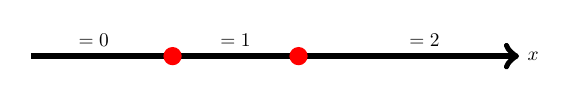
\begin{tikzpicture}[scale=0.2,every node/.style={scale=0.7}]
\draw[->,line width=0.08cm] (-5,0)--(26,0) node[right]{$\glssymbol{x}$};

\node [red,circle, fill] at (4,0) {};
\node [red,circle, fill] at (12,0) {};

\node at (-1,1) {$\E = 0$};
\node at (8,1) {$\E = 1$};
\node at (20,1) {$\E = 2$};
\end{tikzpicture}
\end{minipage}

\vfill

\begin{minipage}{0.45\textwidth}
\centering
\caption{\label{fig:disc_disc} Discrétisation d'une variable qualitative.}
\begin{tikzpicture}[scale=0.2,every node/.style={scale=0.7}]
\tikzset{vertex/.style = {shape=circle,draw,scale=0.7,minimum size=1cm}}
\tikzset{edge/.style = {->,> = latex'}}

% Boules E^j
\node [vertex] (e1) at (3,2.5) {0};
\node [vertex] (e2) at (15,2.5) {1};

% Boules X^J
\node [vertex] (x1) at (-4,0) {0};
\node [vertex] (x2) at (1.8,0) {1};
\node [vertex] (x3) at (9.5,0) {2};
\node [vertex] (x4) at (17,0) {3};
\node [vertex] (x5) at (24,0) {4};

% Labels
\node at (-7,2.5) {$\E=$};
\node at (-7,0.2) {$\glssymbol{X}=$};

% Flèches
\draw[edge,line width=0.03cm] (x1) to (e1);
\draw[edge,line width=0.03cm] (x3) to (e1);
\draw[edge,line width=0.03cm] (x4) to (e1);
\draw[edge,line width=0.03cm] (x2) to (e2);
\draw[edge,line width=0.03cm] (x5) to (e2);

\end{tikzpicture}
\end{minipage}
\end{multicols}
\end{figure}


\bigskip

Ce chapitre.


\printbibliography[heading=subbibliography, title=Références du chapitre 3]

